\documentclass[10pt,english]{article}

\usepackage{fourier}

\usepackage[]{graphicx}
\usepackage[]{color}
\usepackage{xcolor}
\usepackage{alltt}
\usepackage{listings}
\usepackage[T1]{fontenc}
\usepackage[utf8]{inputenc}
\setlength{\parskip}{\smallskipamount}
\setlength{\parindent}{5ex}
\usepackage{indentfirst}
\usepackage{listings}
\usepackage{setspace}
\usepackage{hyperref}
\hypersetup{
    colorlinks=true,
    linkcolor=auburn,
    filecolor=magenta,      
    urlcolor=blue, urlsize=2em
}

% Set page margins
\usepackage[top=100pt,bottom=100pt,left=68pt,right=66pt]{geometry}

% Package used for placeholder text
\usepackage{lipsum}

% Prevents LaTeX from filling out a page to the bottom
\raggedbottom


\usepackage{fancyhdr}
\fancyhf{} 
\fancyfoot[C]{\thepage}
\renewcommand{\headrulewidth}{0pt} 
\pagestyle{fancy}

\usepackage{titlesec}
\titleformat{\chapter}
   {\normalfont\LARGE\bfseries}{\thechapter.}{1em}{}
\titlespacing{\chapter}{0pt}{50pt}{2\baselineskip}

\usepackage{float}
\usepackage{verbatim}
\floatstyle{plaintop}
\restylefloat{table}

\usepackage[tableposition=top]{caption}


\definecolor{light-gray}{gray}{0.95}

\renewcommand{\contentsname}{Índice}

\begin{document}


\begin{titlepage}
	\clearpage\thispagestyle{empty}
	\centering
	\vspace{2cm}

	
	{\Large  Segurança Informática e nas Organizações \par}
	\vspace{0.5cm}
	{\small Professor: \\
	João Paulo Barraca\par}
	\vspace{4cm}
	{\Huge \textbf{Gestão de direitos digitais}} \\
	\vspace{1cm}
	\vspace{4cm}
	{\normalsize Hugo Paiva, 93195 \\ 
	             Luís Valentim, 93989
	   \par}
	\vspace{2cm}

    
\includegraphics[scale=0.20]{logo_ua.png}
    
    \vspace{2cm}
    
	{\normalsize DETI \\ 
		Universidade de Aveiro \par}
		
	{\normalsize 30-12-2020 \par}
	\vspace{2cm}
		
	
	\pagebreak

\end{titlepage}
\tableofcontents{}
\clearpage

\section{Introdução}
\par Este trabalho projeto tem como objetivo o desenvolvimento de mecanismos de proteção de dados e comunicações num serviço cliente servidor.

\par Neste sentido, foi fornecido a estrutura base do serviço com algumas funções relativas aos protocolos de comunicação desprotegidos já implementadas e coube-nos a nós desenvolver as capacidades de proteção da troca de informação nomeadamente através de encriptação das comunicações, com protocolos previamente acordados entre o cliente e o servidor, e do repositório de músicas, bem como os processos inversos de desencriptação consequentes e ainda os protocolos de autentificação, e troca de chaves assimétricas tanto do cliente como do servidor. 

\par Este relatório visa explicar os protocolos escolhidos para cada problema,o porque dessas escolhas e a forma como os mesmos foram implementados.
\clearpage

\section{Cifra das comunicações}
\subsection{Protocolo}
 \par Com o objetivo de cifrar as comunicações cliente-servidor, foi definido um protocolo que dita qual o tipo de cifra, o algoritmo que a mesma usa, o modo de cifra e qual o algoritmo de \textit{hash} utilizado para gerar assinaturas e outros dados.

\par Optando pela Cifra Simétrica para as comunicações, foi escolhido um leque de opções de entre alguns modos de cifra, algoritmos de \textit{hash} e algoritmos de cifra que posteriormente é utilizado para escolher de forma aleatória um deles para utilização na comunicação. As opções disponíveis são:

\begin{itemize}
    \item {\textbf{Algoritmos de Cifra}} - \textit{AES} e  \textit{Camellia}
   
   \item {\textbf{Algoritmos de \textit{hash}}} - \textit{SHA256} e \textit{SHA3\_256}
  
\item {\textbf{Modos de Cifra}} - \textit{CTR}, \textit{OFB} e \textit{CFB}
    
 \end{itemize}
 
 \par Em ambos as aplicações, Cliente e Servidor, o leque de opções é definido da seguinte forma:
 
  \begin{figure}[!h]
        \centering
        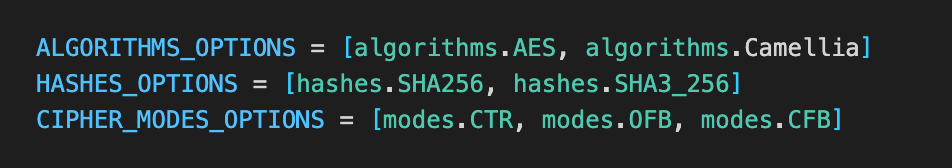
\includegraphics[width=250]{images/cipher_suite.png}
        \caption{Leque de opções mencionado}
    \end{figure}
 
 \par Ao executar o cliente, a primeira comunicação com o servidor é o envido das opções. De entre o leque de opções de cada tipo, é gerado aleatoriamente o número de opções enviado para o servidor, podendo, por exemplo, para as opções de algoritmos de cifra, enviar ambos os algoritmos ou apenas um deles. Após esta decisão, são escolhidos aleatoriamente os algoritmos, sem repetição, até chegar ao número gerado anteriormente, podendo, portanto, enviar apenas o algoritmo \textit{AES} ou apenas o \textit{Camellia} ou ambos. Para os modos de cifra e algoritmos de \textit{hash} a escolha é feita de maneira semelhante: 

  \begin{figure}[!h]
        \centering
        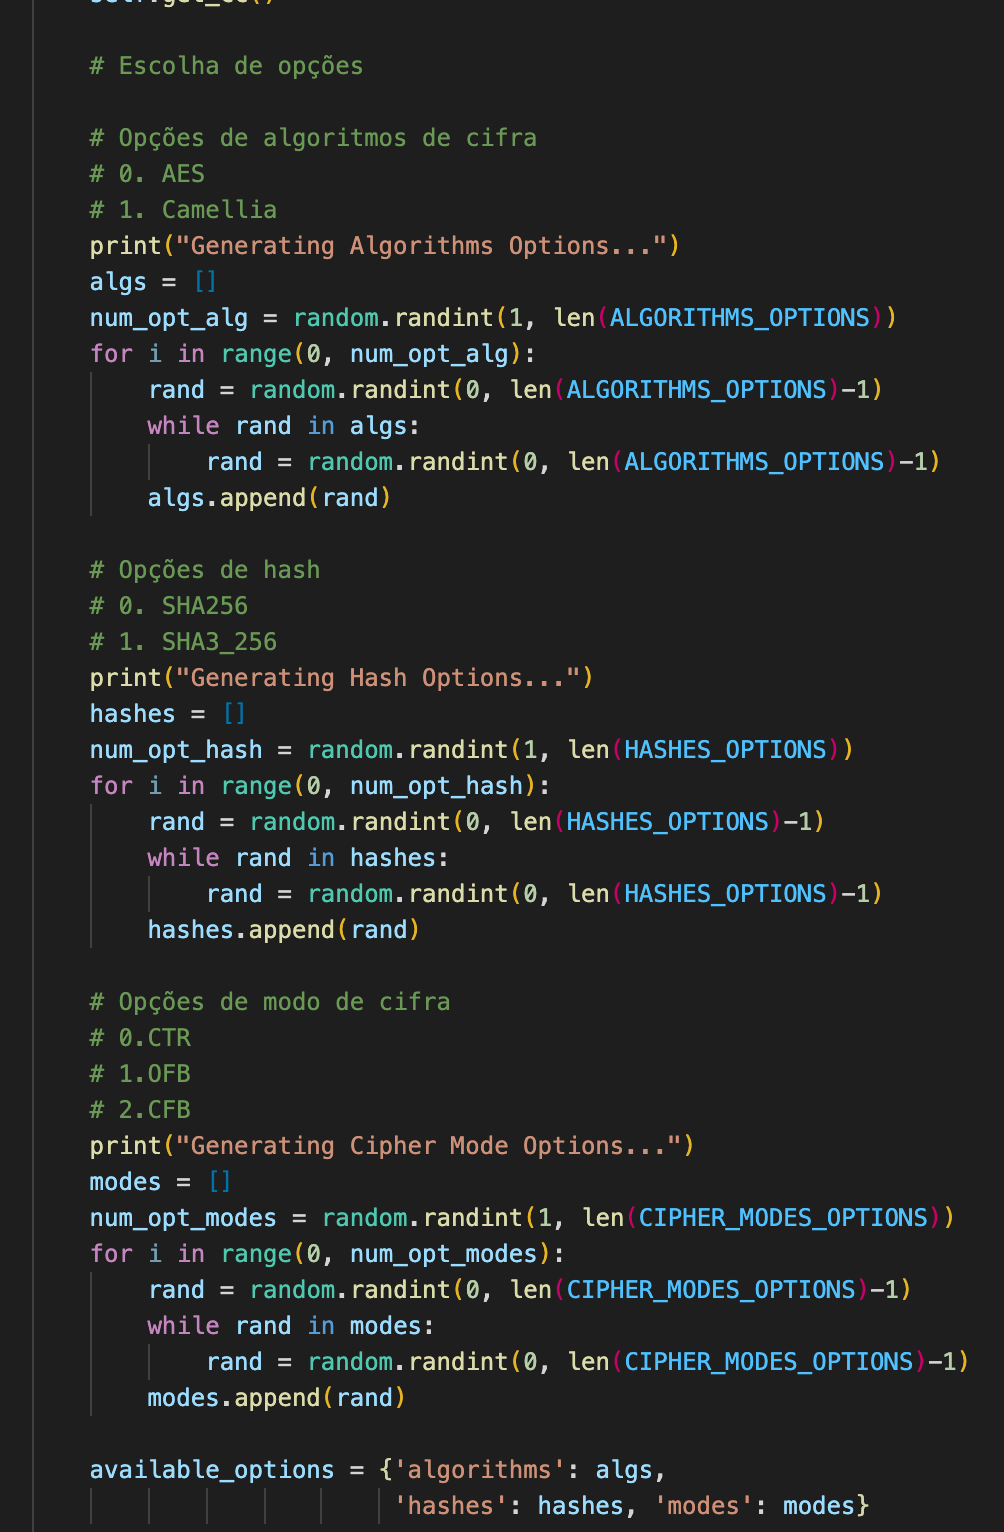
\includegraphics[width=250]{images/cipher_suite_decision_client.png}
        \caption{Escolha do leque de opções para enviar ao servidor}
    \end{figure}
    
    \clearpage
    
\par Ao enviar este leque de opções, o cliente identifica-se através do \textit{header} \textit{Authorization} com um \textit{uuid} gerado previamente, passando a utilizá-lo em todas as comunicações como seu identificador. O servidor, ao receber estas opções, escolhe aleatoriamente quais pretende utilizar e responde ao cliente com essa informação, ficando essa informação guardada em ambas as aplicações:

\begin{figure}[!h]
        \centering
        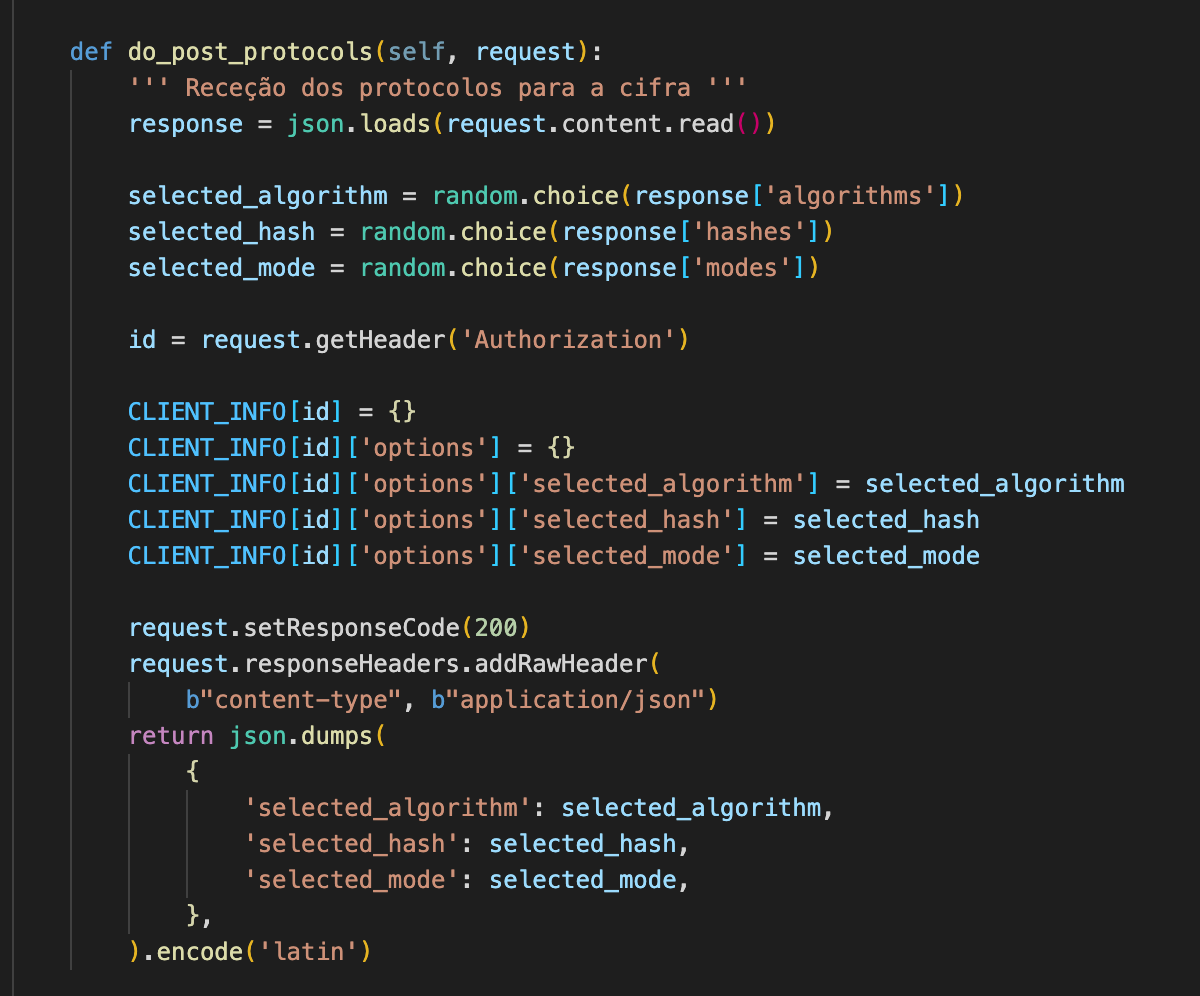
\includegraphics[width=250]{images/cipher_suite_decision_server.png}
        \caption{Escolha das opções finais por parte do servidor}
\end{figure}

\begin{figure}[!h]
        \centering
        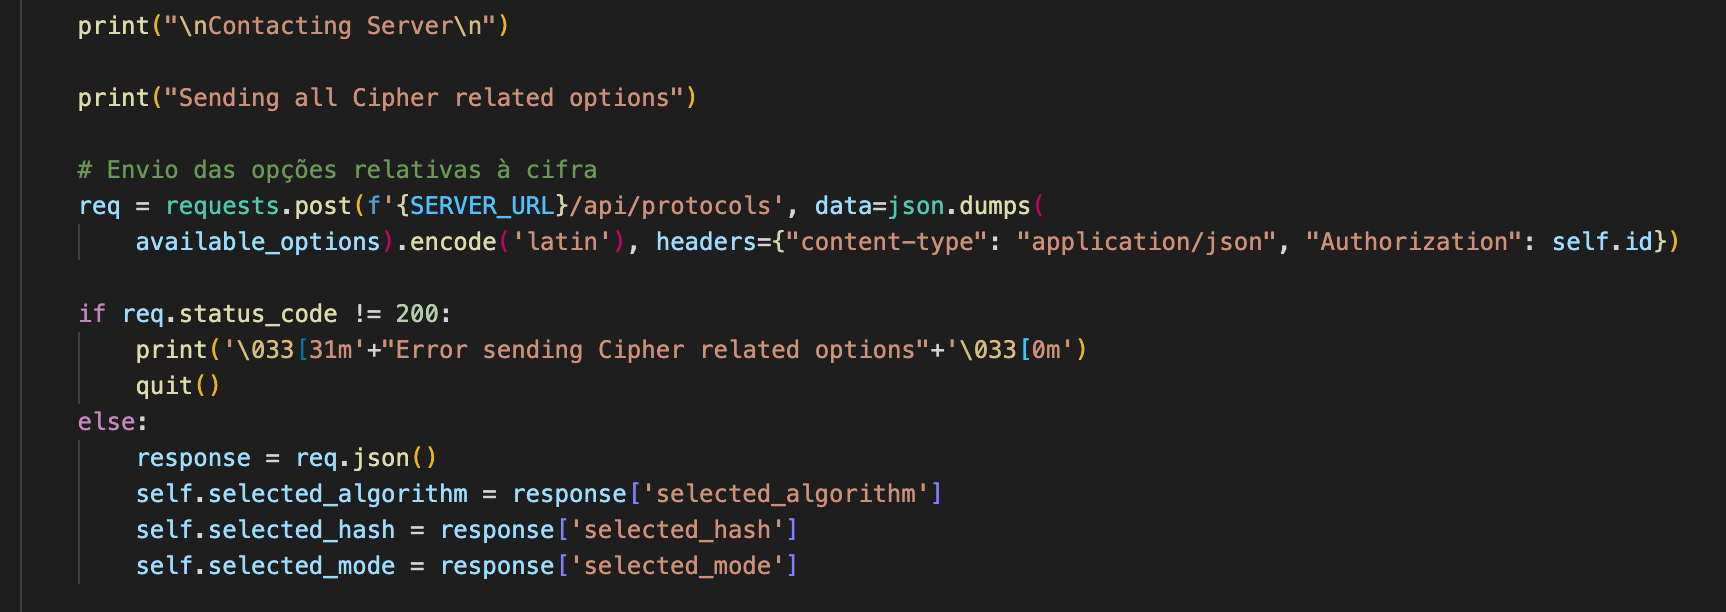
\includegraphics[width=250]{images/cipher_suite_save_client.png}
        \caption{Informação do protocolo guardada no cliente}
\end{figure}

\subsection{Troca de chaves}

\par Para ser possível cifrar as mensagens após a troca do protocolo é necessário a geração e troca de chaves simétricas. Como a comunicação está em aberto foi necessário recorrer a um algoritmo que permite a geração de um segredo partilhado em um canal inseguro, como é o caso, sem problemas de segurança, tal como foi abordado nas aulas teóricas com o algoritmo \textit{Diffie-Hellman}. Para evitar os problemas de um ataque \textit{Man-In-The-Middle} que este algoritmo tem, foi utilizada a forma efêmera do mesmo, disponível no \textit{cryptography.io}.

\par Foram trocadas duas chaves, uma para ser utilizada na criptografia das comunicações e outras para ser utilizada na geração das assinaturas das comunicações com base em \textit{HMAC}. Para gerar as chaves foram criadas duas funções no cliente utilizando as implementações do \textit{cryptography.io}:

\begin{figure}[!h]
        \centering
        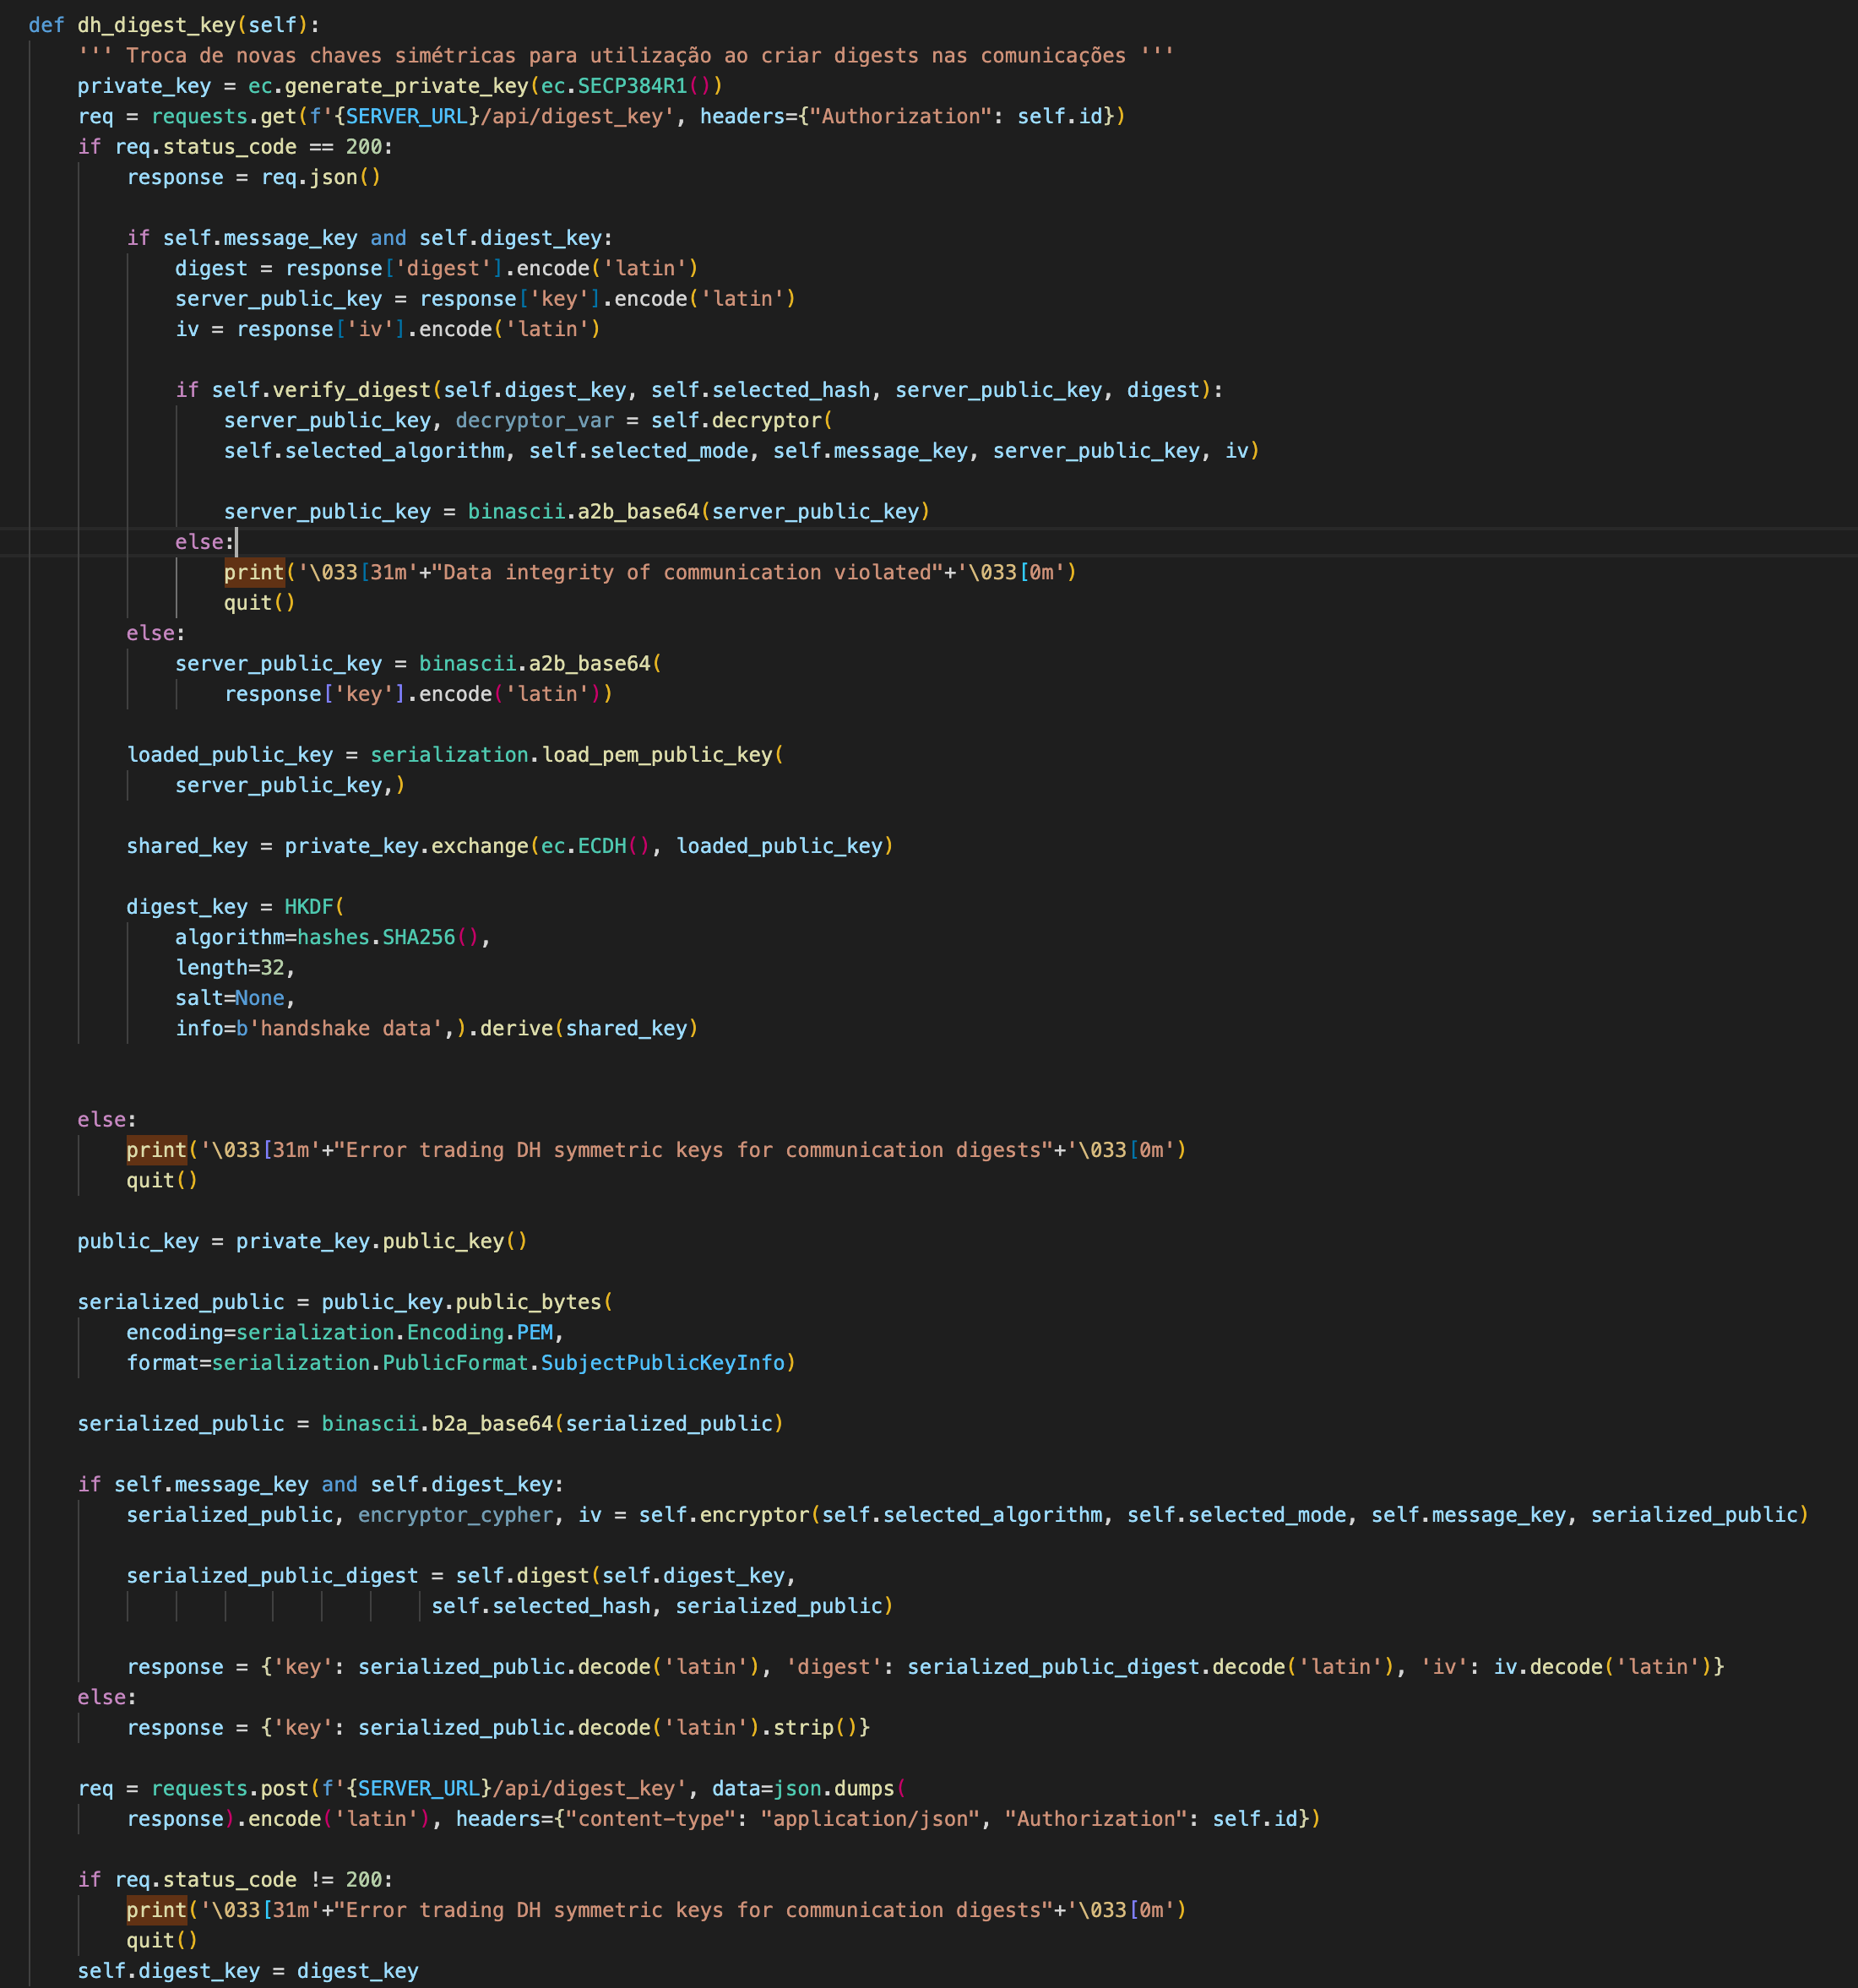
\includegraphics[width=400]{images/dh_digest_client.png}
        \caption{Geração do segredo partilhado para utilizar no \textit{HMAC}, no cliente}
\end{figure}

\begin{figure}[!h]
        \centering
        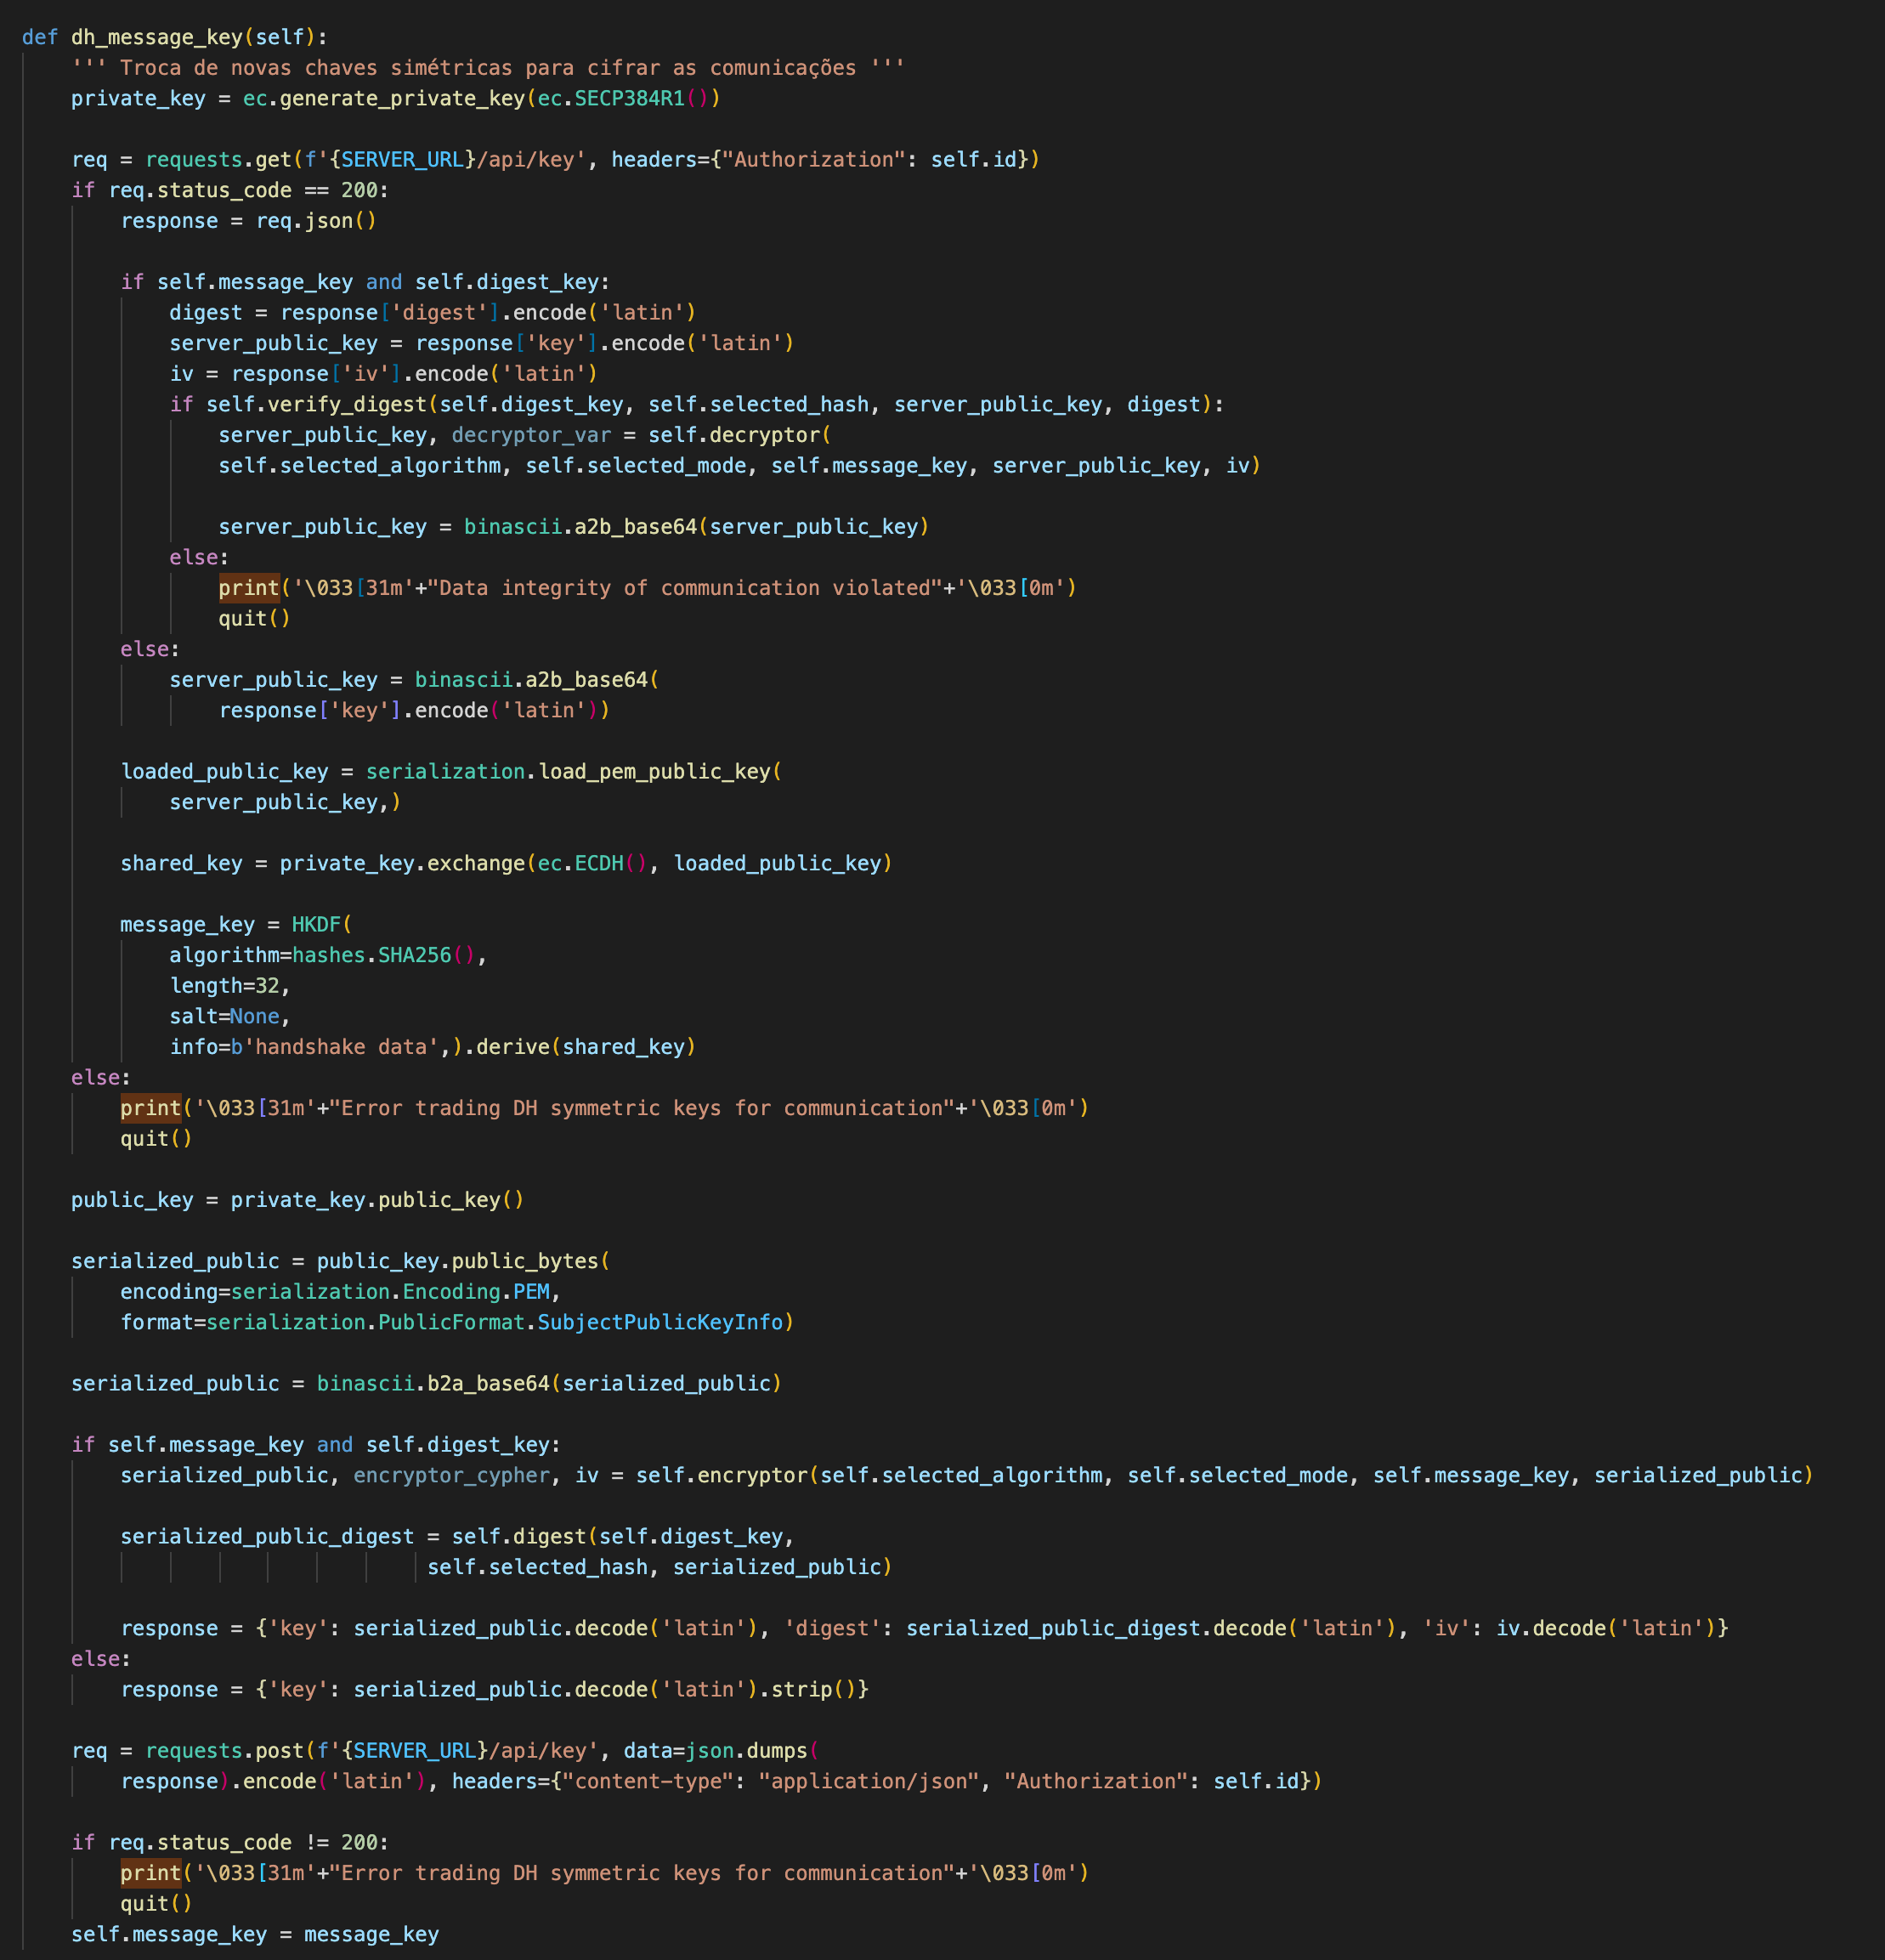
\includegraphics[width=400]{images/dh_message_client.png}
        \caption{Geração do segredo partilhado para utilizar na criptografia das comunicações, no cliente}
\end{figure}

\clearpage

\par Do lado do servidor o processo é relativamente parecido sendo que, de acordo com a utilização do cliente, primeiro é gerada uma chave pública para ser enviada e posteriormente é recebida a chave pública do cliente, gerando o segredo partilhado que será a chave a utilizar:

\begin{figure}[!h]
        \centering
        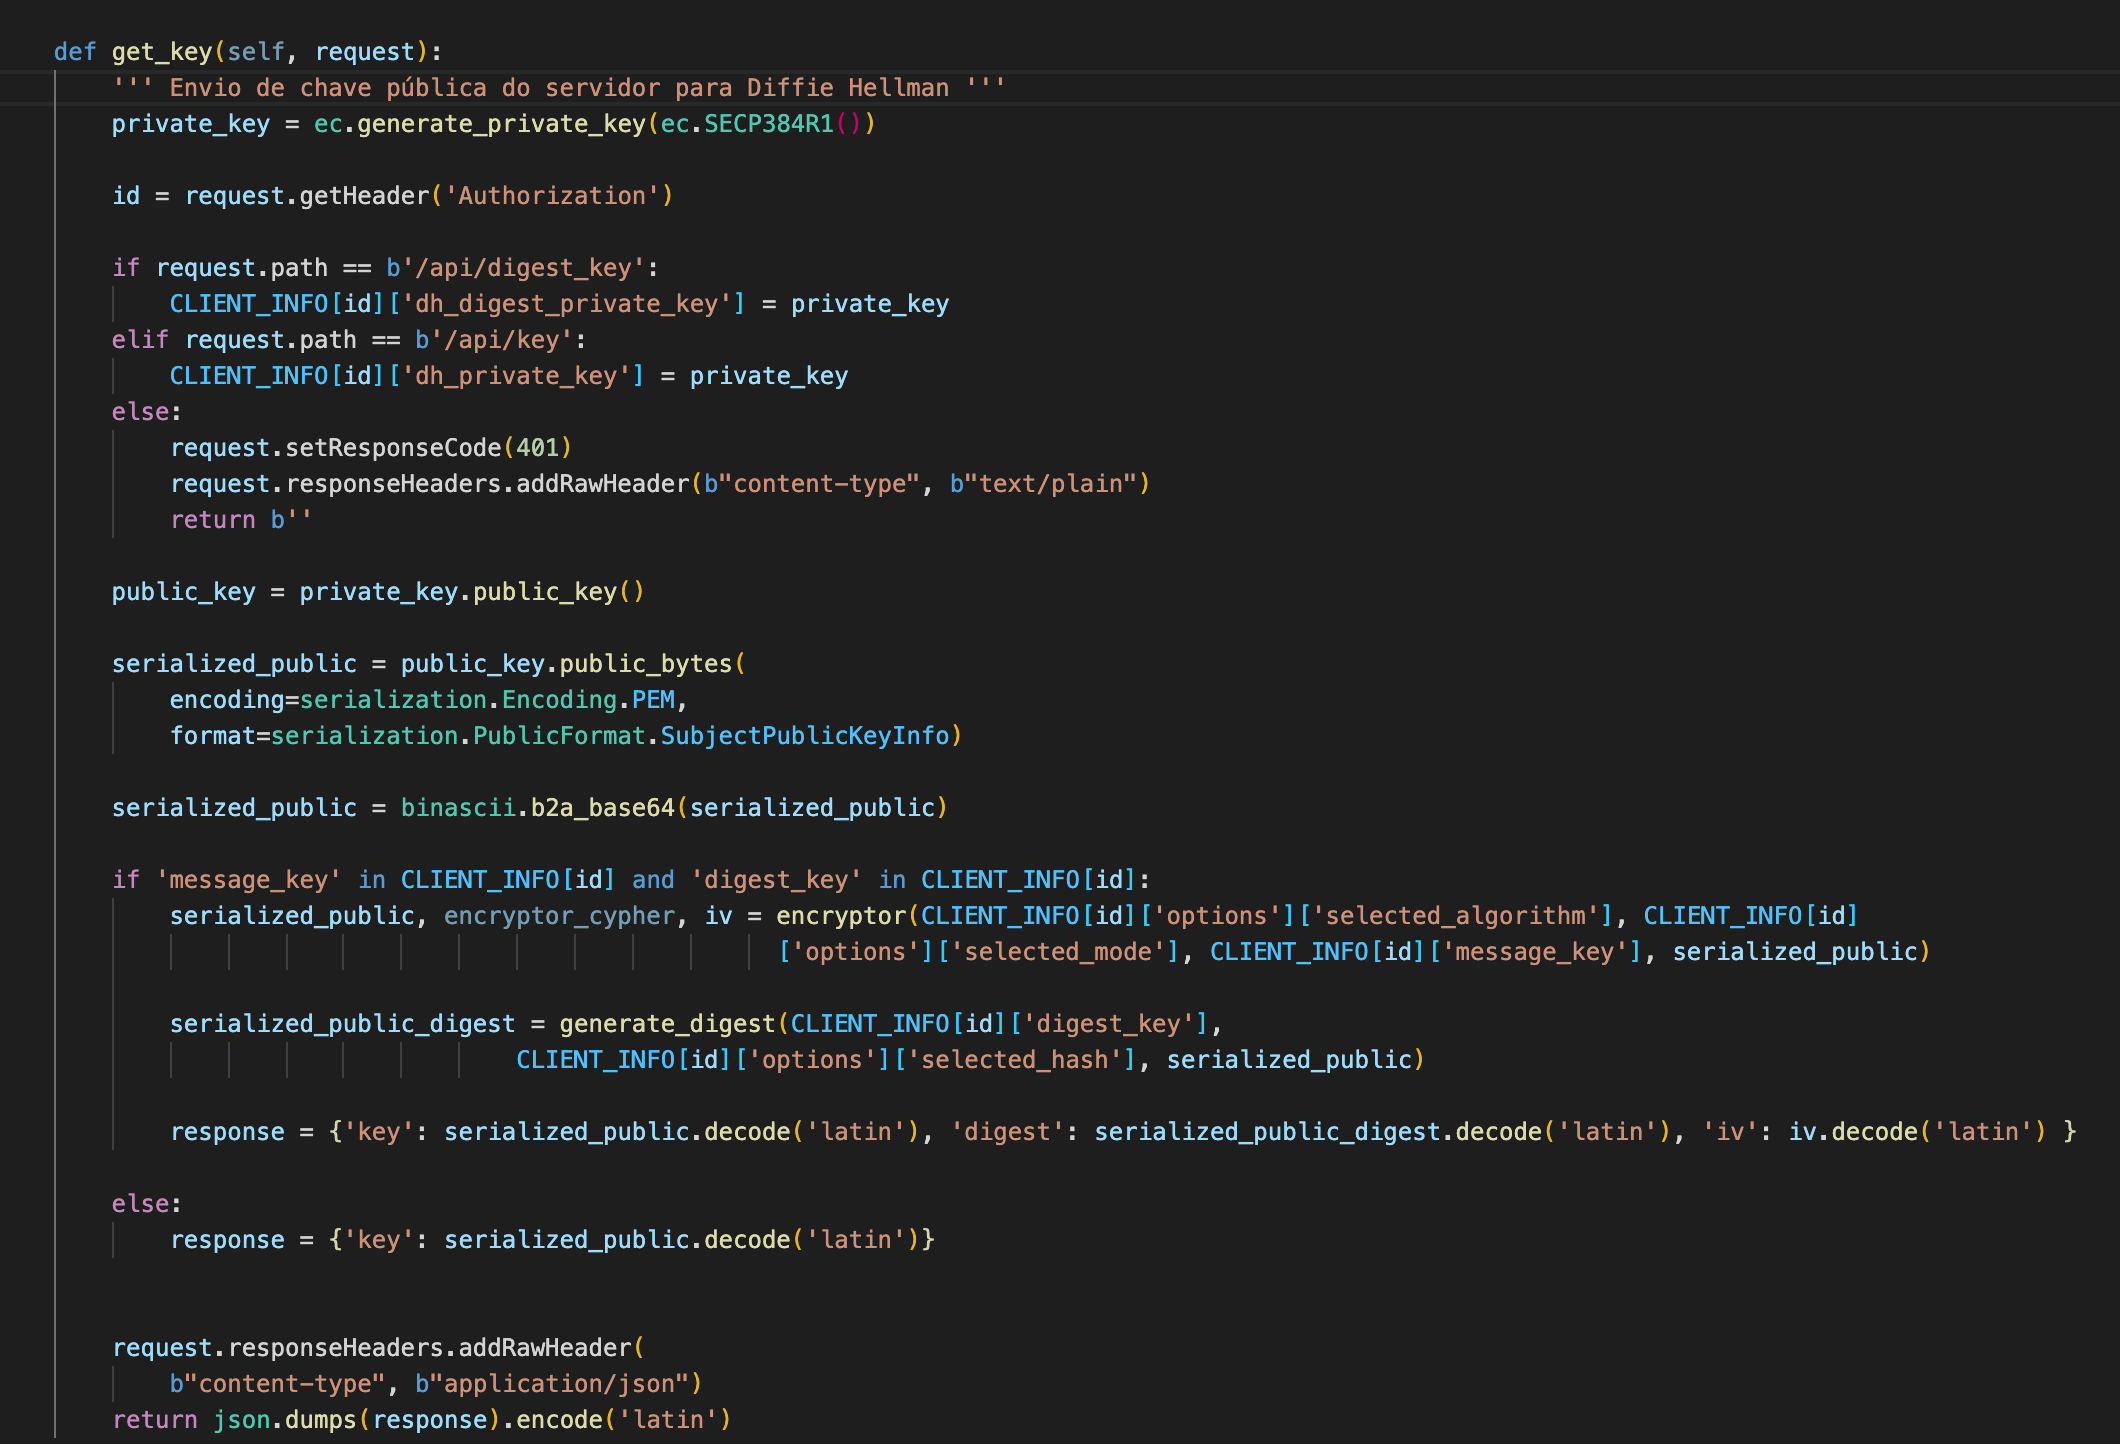
\includegraphics[width=\textwidth]{images/dh_send_server.png}
        \caption{Geração da chave pública para enviar ao cliente, no servidor}
\end{figure}

\begin{figure}[!h]
        \centering
        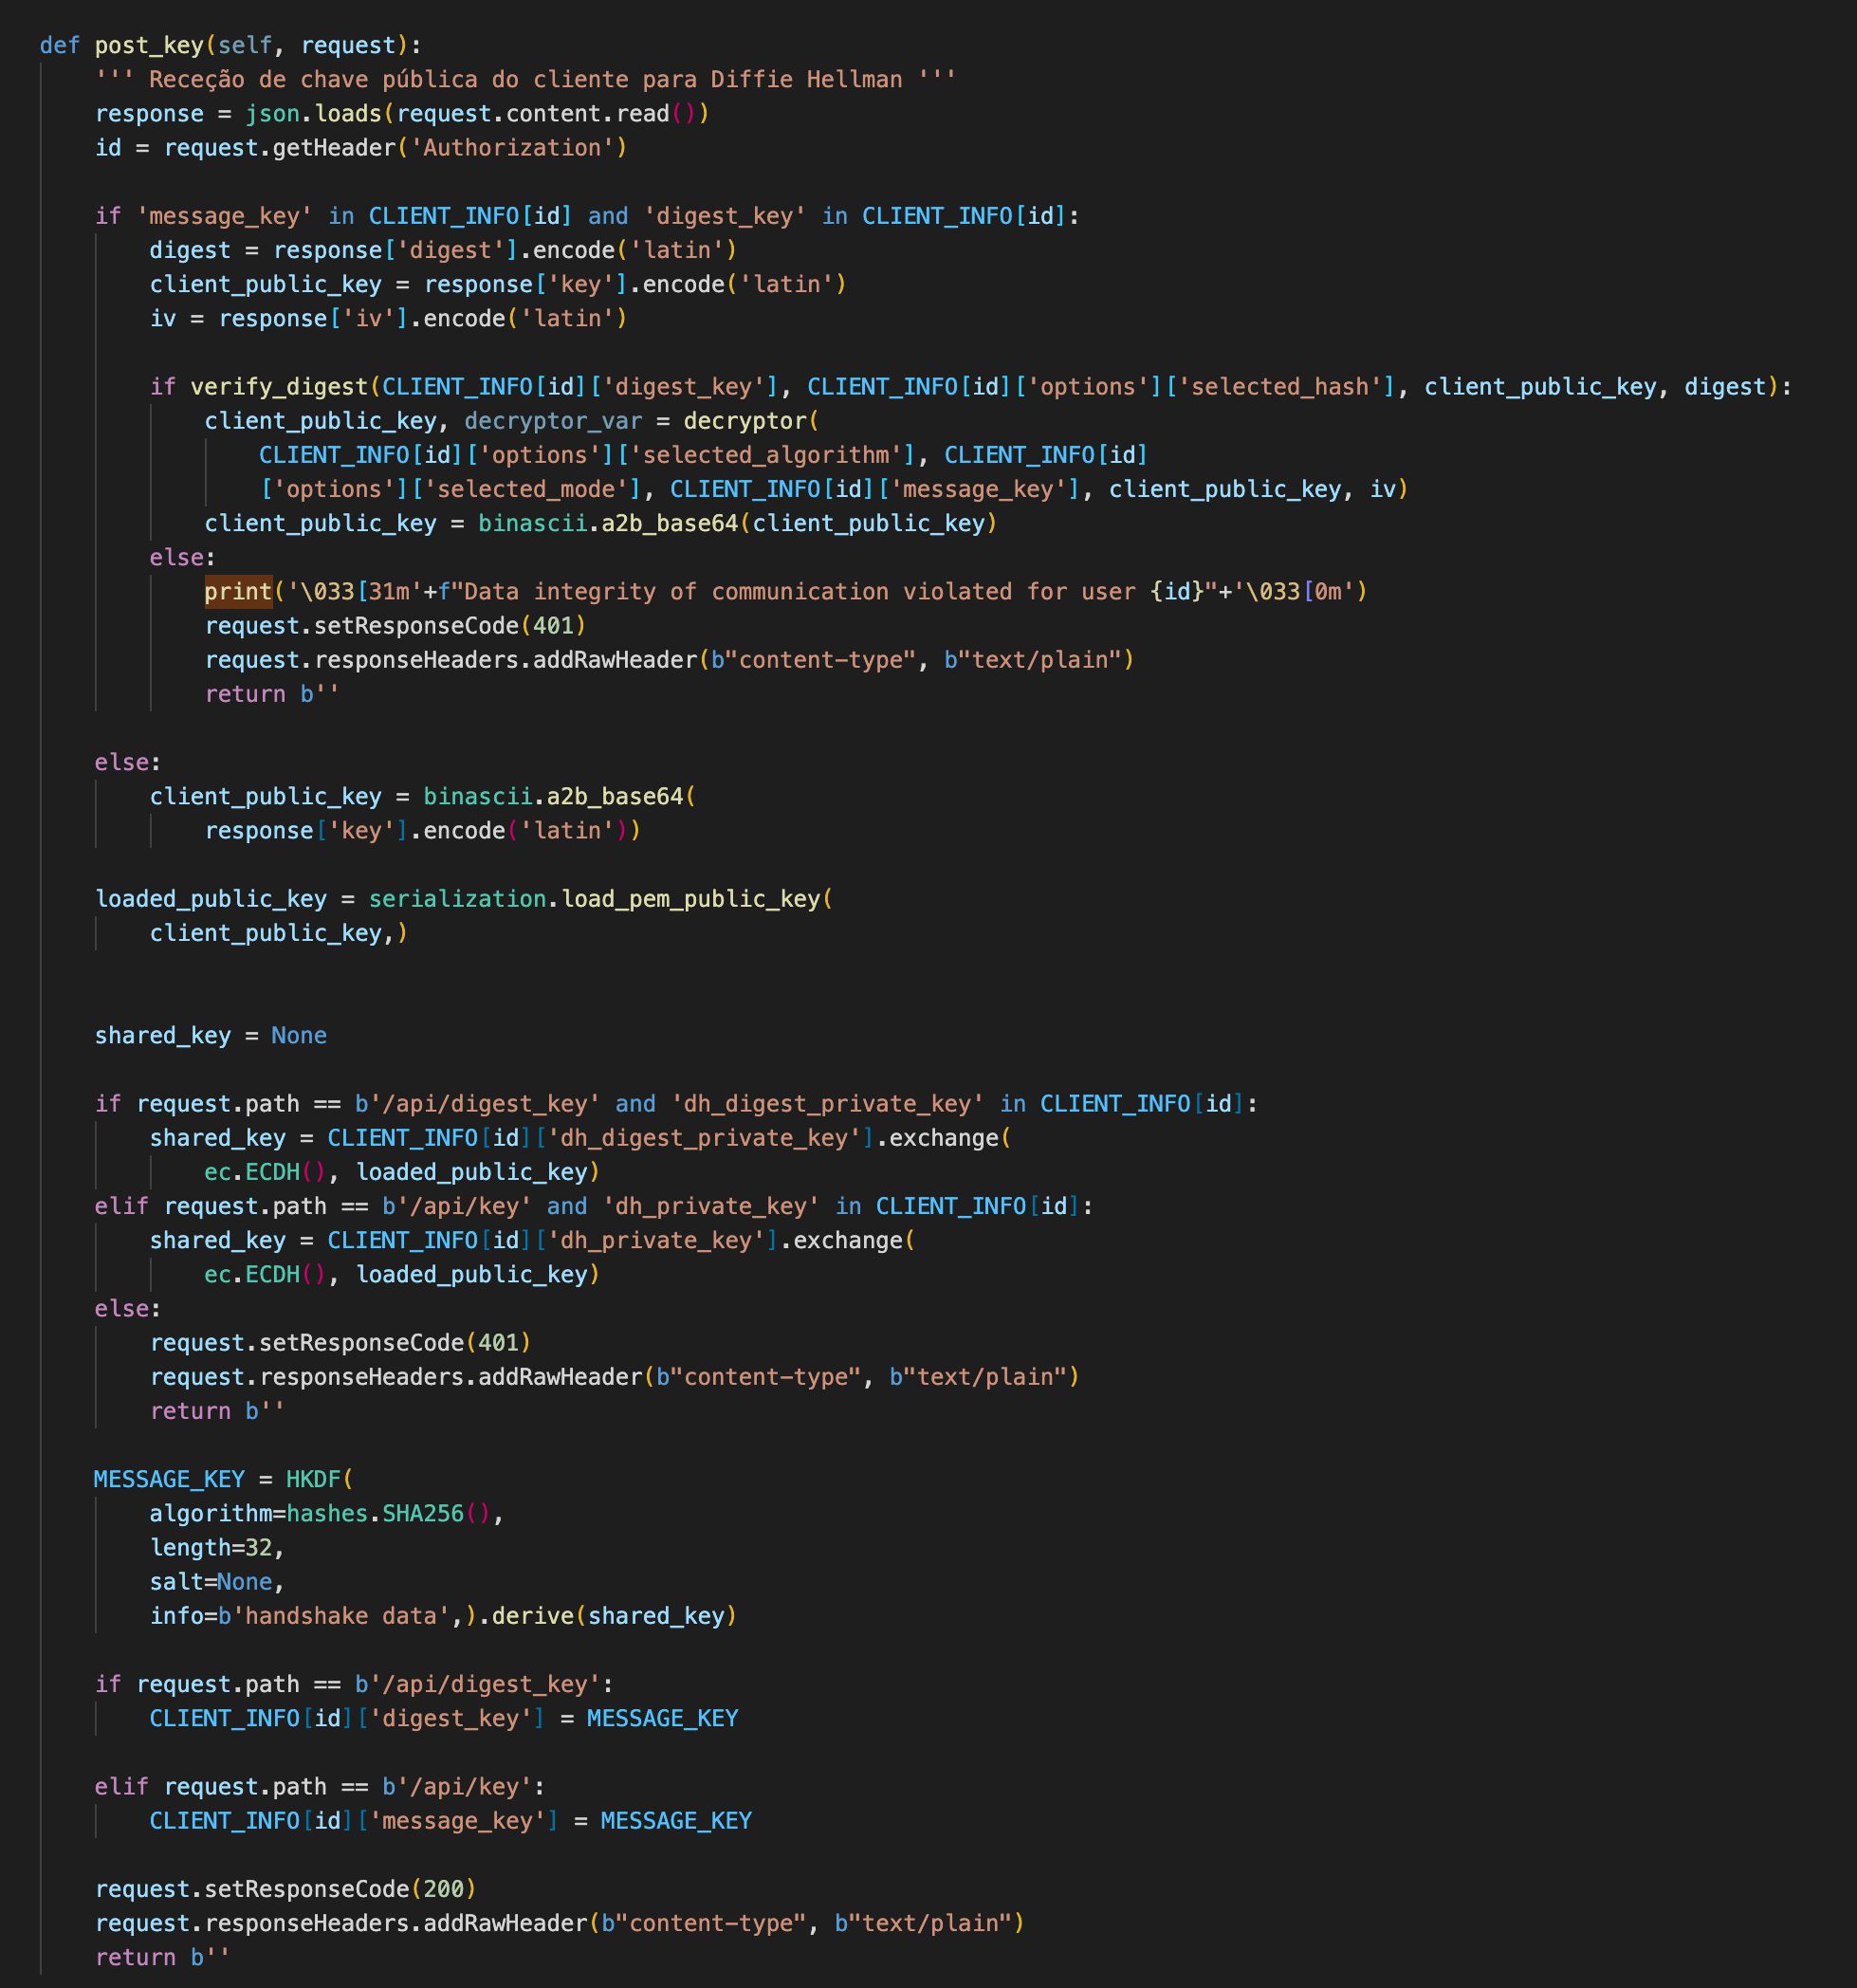
\includegraphics[width=\textwidth]{images/dh_get_server.png}
        \caption{Geração do segredo partilhado de acordo com a chave pública recebida do cliente, no servidor}
\end{figure}

\clearpage

\par Visto que a troca de chaves também irá acontecer já depois do protocolo da cifra estar definido, como será explicado posteriormente, estas funções permitem enviar a chave pública em aberto quando o protocolo ainda não está definido mas, também enviam cifrada, caso o protocolo e as chaves já estejam definidas. Mais uma vez, toda esta troca tem como base o \textit{uuid} do cliente referido anteriormente e que é utilizado pelo servidor para guardar as informações necessárias no dicionário \textit{CLIENT\_INFO}.



\subsection{Cifra das comunicações e Validação da integridade}

\par Tendo o protocolo e as chaves trocadas, o servidor e o cliente passam a comunicar de forma encriptada. Em ambas as aplicações foram criadas funções para encriptar, desencriptar e validar a integridade de mensagens. A implementação da função de encriptação do lado do cliente é a única que difere da do lado do servidor pois não necessita de permitir encriptar novamente a partir do \textit{encryptor} de uma encriptação anterior, sendo que isto é utilizado para permitir o fluxo correto do \textit{iv} e outras propriedades, dependendo do modo de cifra. Esta diferença cai no facto de que o cliente apenas cifra mensagens que não são divididas em vários blocos, ao contrário do servidor que cifra os vários blocos das músicas, necessitando de guardar e manter o fluxo das propriedades daquela cifra em específico para não ser necessário enviar um novo \textit{iv} em todos os blocos encriptados da música.


\par As implementações das funções são as seguintes:

\begin{figure}[!h]
        \centering
        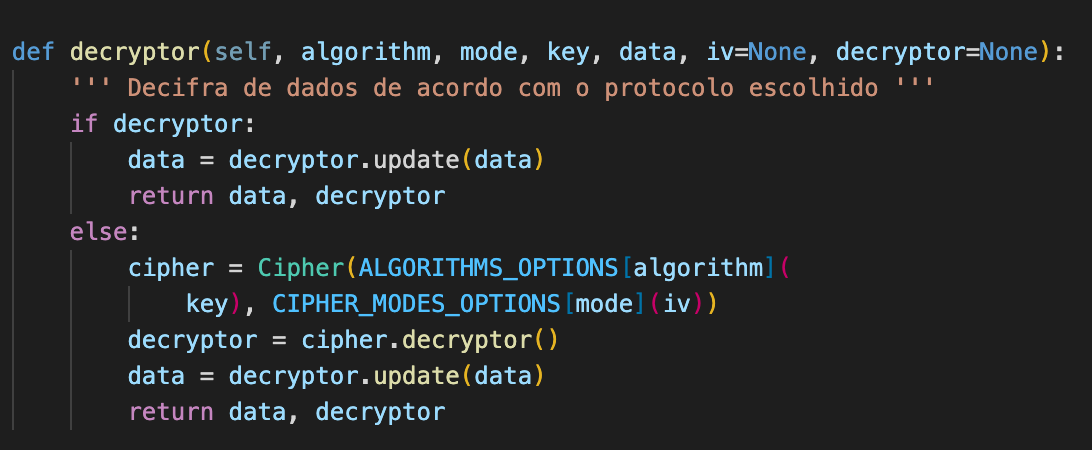
\includegraphics[width=275]{images/decryptor.png}
        \caption{Função de desencriptação, igual em ambas as aplicações}
\end{figure}

\begin{figure}[!h]
        \centering
        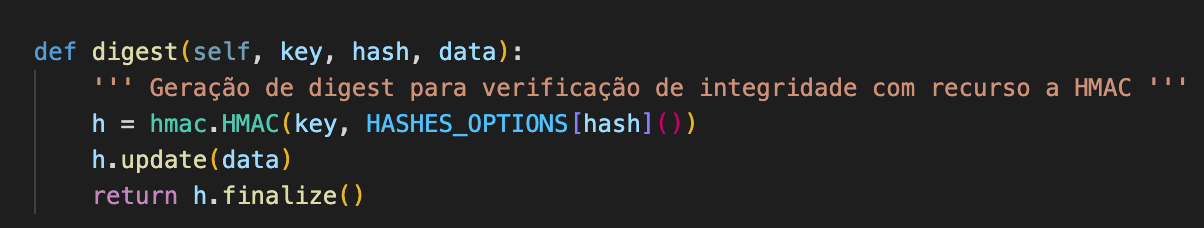
\includegraphics[width=275]{images/digest.png}
        \caption{Função que gera uma espécie de \textit{digest}, uma assinatura, utilizando uma chave, permitindo validar a integridade e autenticidade de dados, tal como referido na especificações do \textit{HMAC}}
\end{figure}

\begin{figure}[!h]
        \centering
        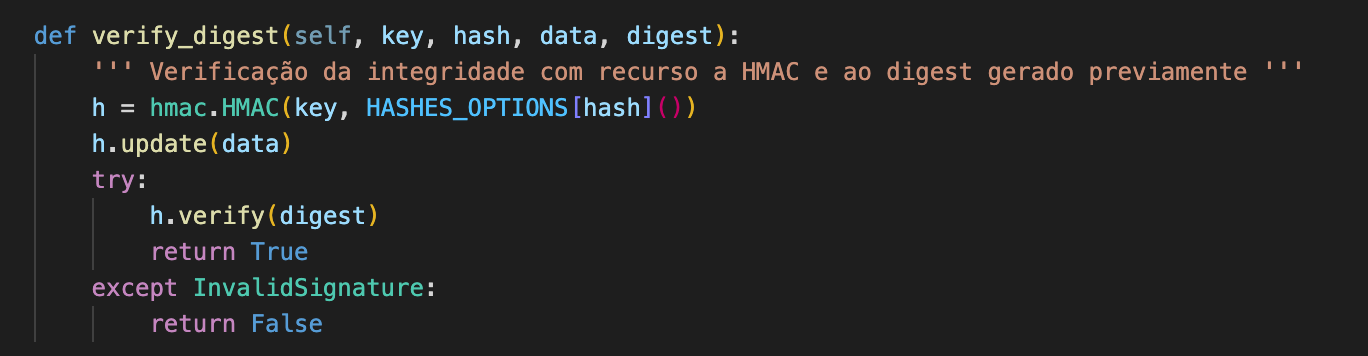
\includegraphics[width=275]{images/verify_digest.png}
        \caption{Função que permite verificar a assinatura dos dados passados, passando também a respectiva assinatura}
\end{figure}

\begin{figure}[!h]
        \centering
        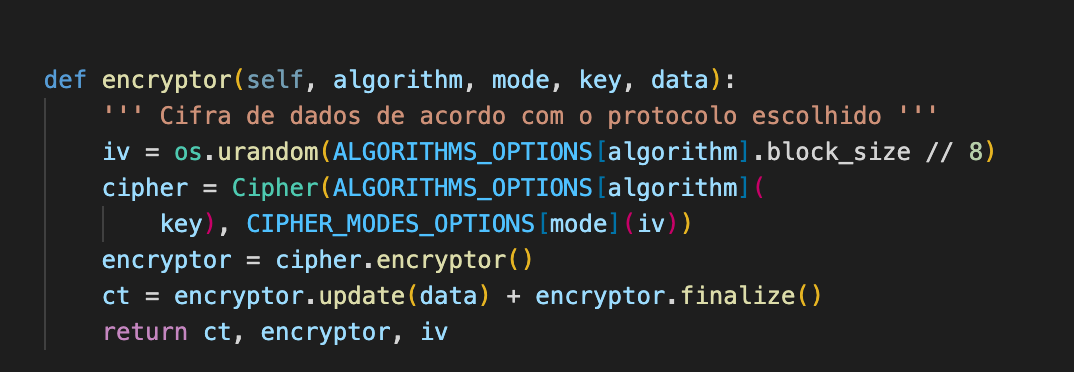
\includegraphics[width=275]{images/encryptor_client.png}
        \caption{Função que permite encriptar dados no cliente}
\end{figure}

\begin{figure}[!h]
        \centering
        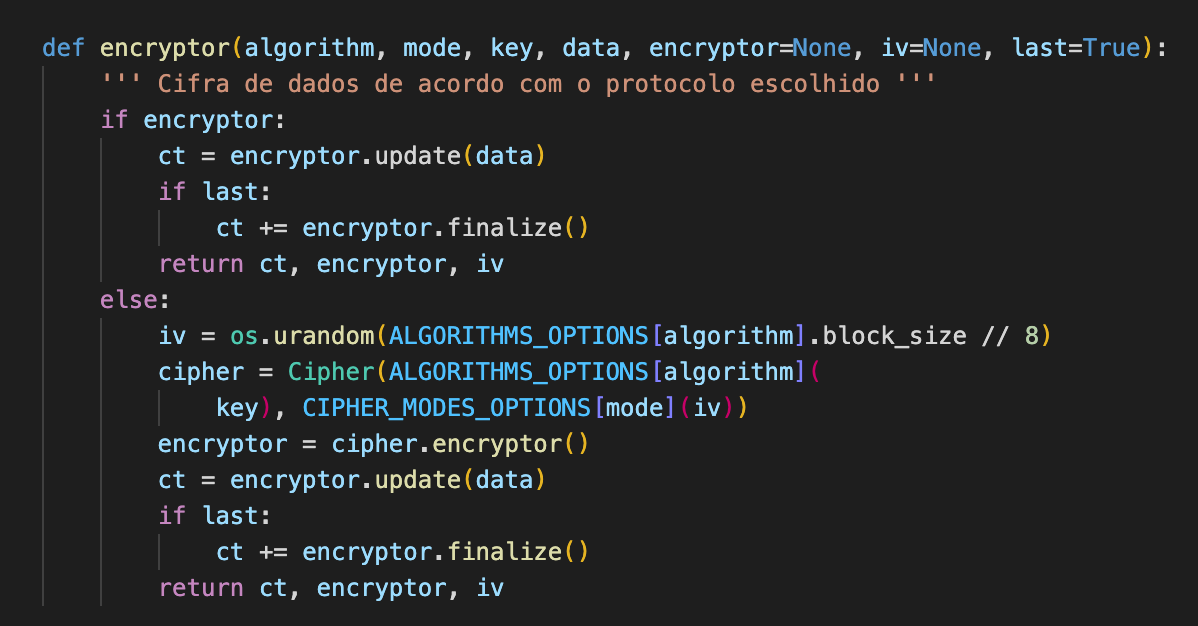
\includegraphics[width=275]{images/encryptor_server.png}
        \caption{Função que permite encriptar dados no servidor}
\end{figure}

\clearpage

\par Aliando todas estas funções é possível cifrar as comunicações, tal como é feito para verificar que o protocolo da cifra, escolhido inicialmente, não foi forjado entretanto:

\begin{figure}[!h]
        \centering
        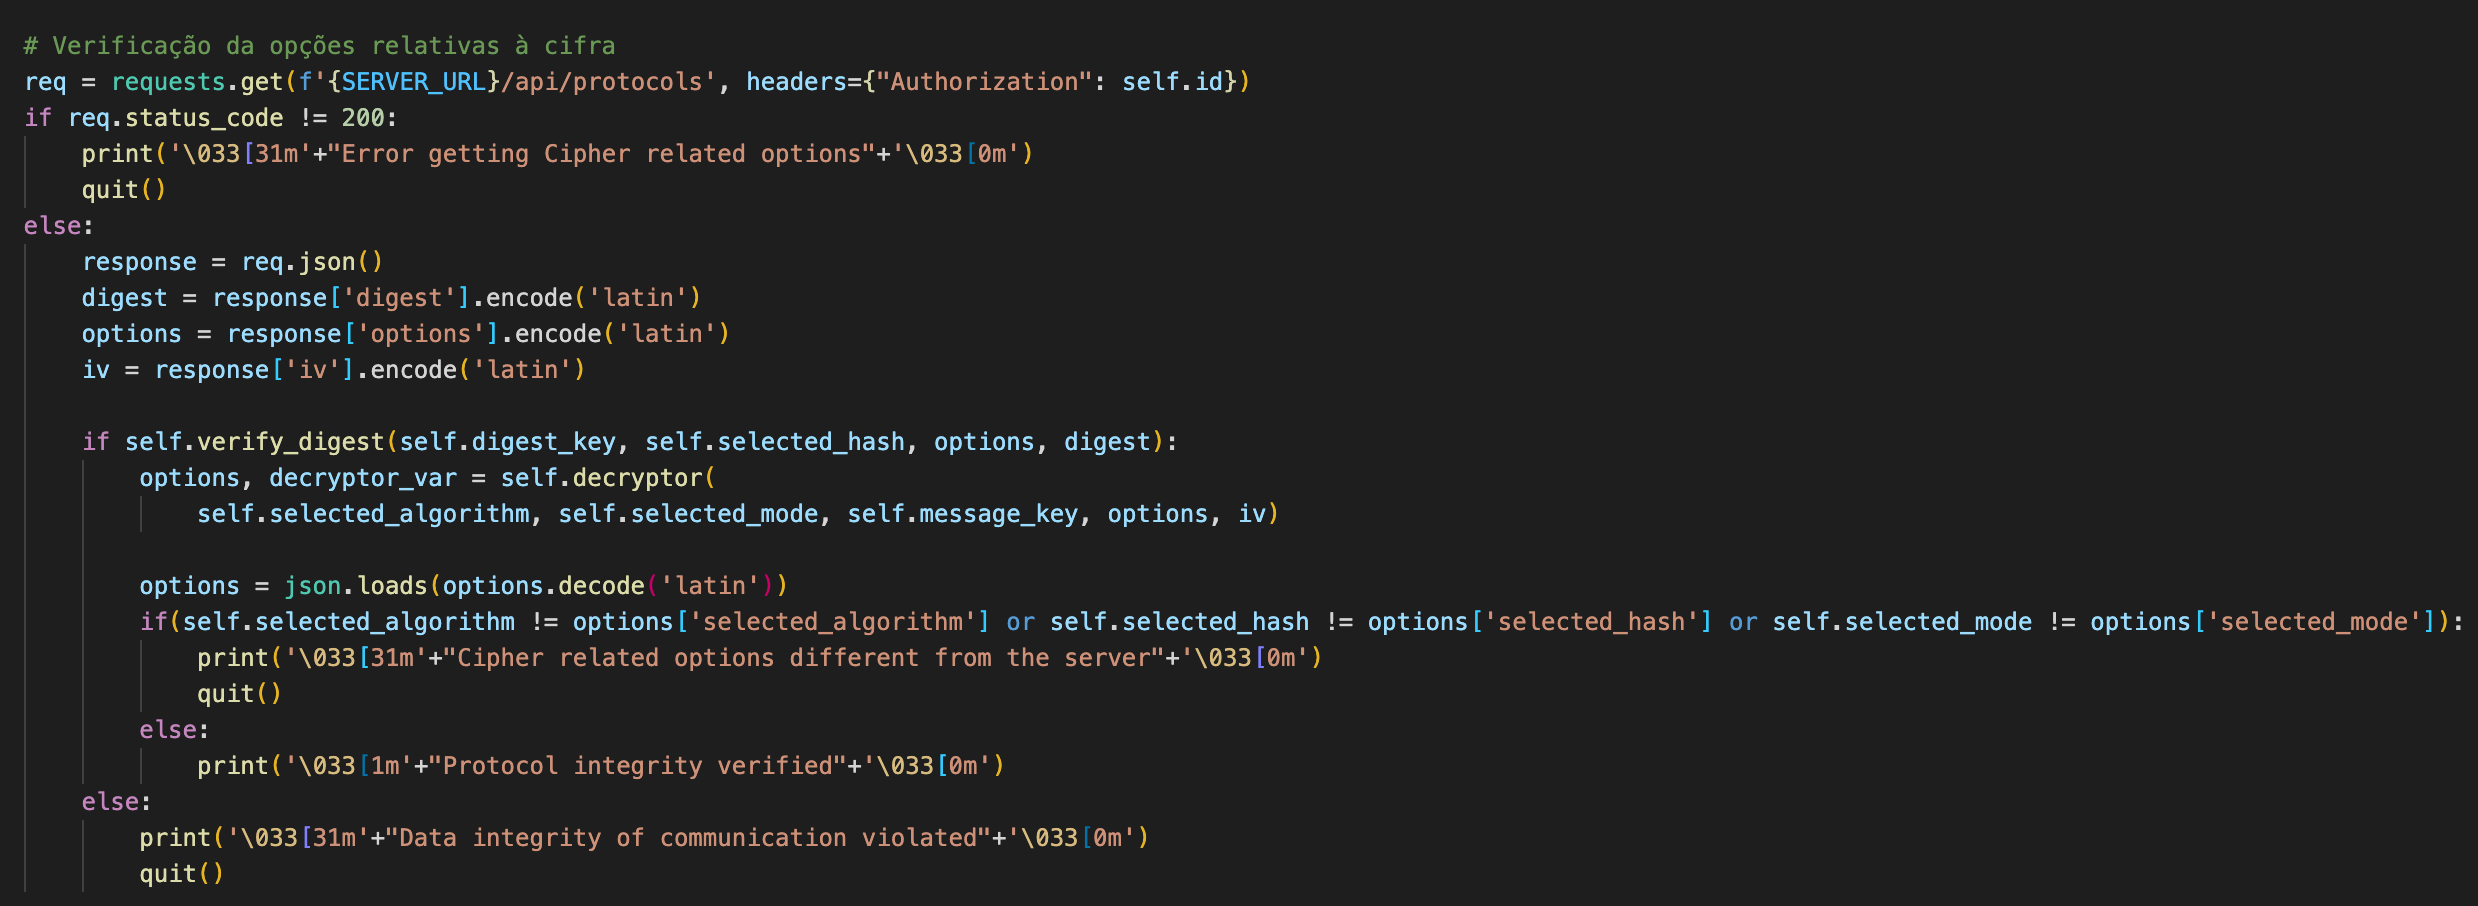
\includegraphics[width=\textwidth]{images/verify_cipher_suite.png}
        \caption{Verificação no cliente que o protocolo da cifra, trocado anteriormente, não foi forjado}
\end{figure}

\par Para a verificação anterior, o cliente pede ao servidor o protocolo da cifra que o mesmo tem guardado. O envio do protocolo é feito da seguinte forma:

\begin{figure}[!h]
        \centering
        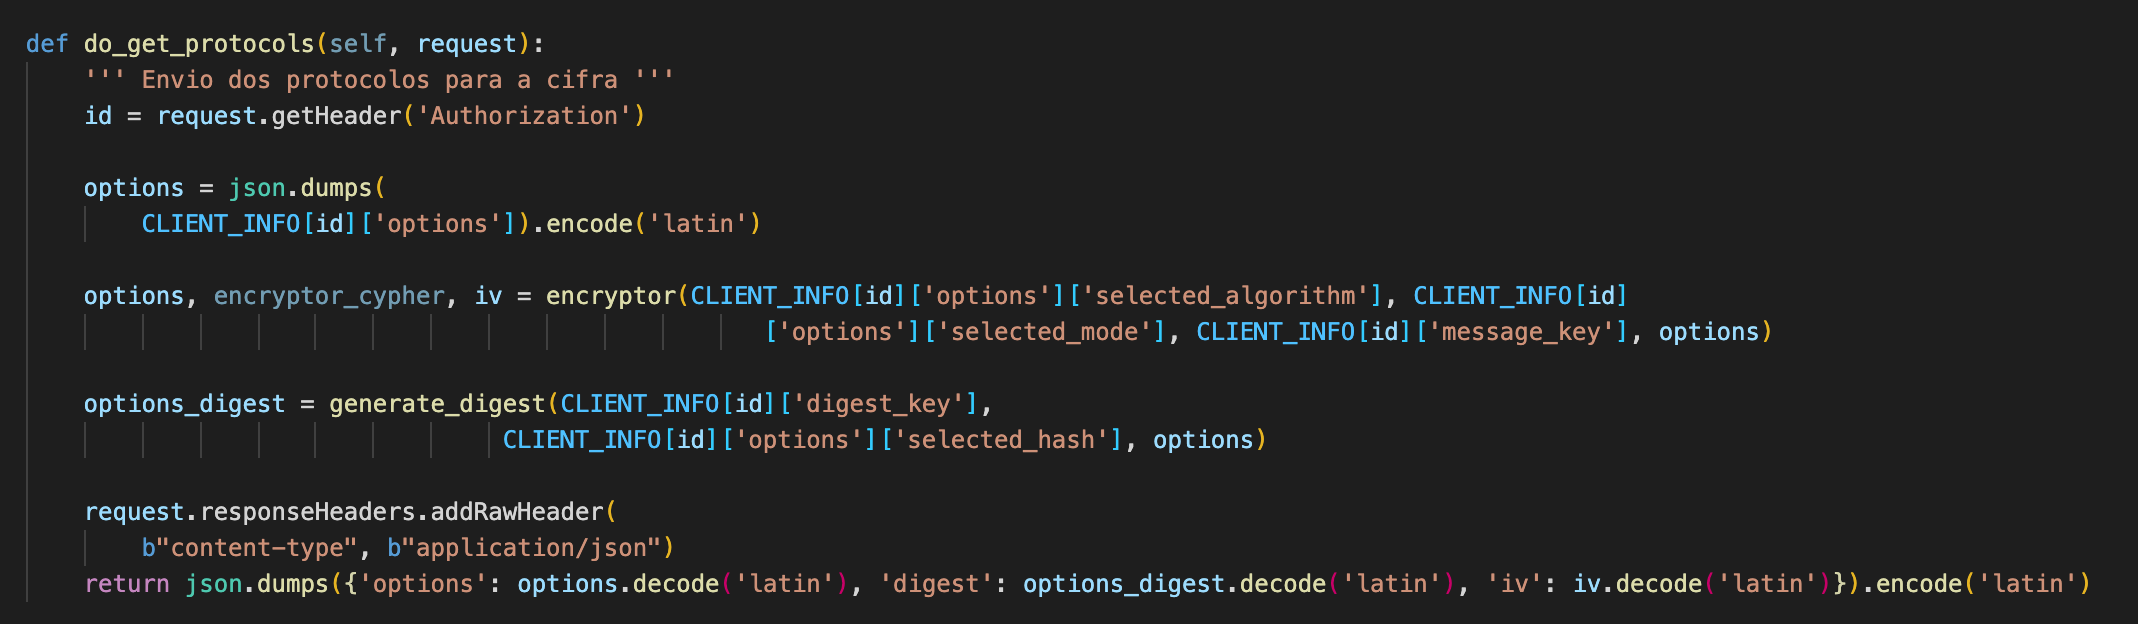
\includegraphics[width=\textwidth]{images/get_cipher_suite.png}
        \caption{Envio do protocolo da cifra definido anteriormente e guardado pelo servidor}
\end{figure}

\par \textbf{Todas as comunicações} a partir deste momento são realizadas de forma similar, permitindo-as ser \textbf{cifradas} e seguras relativamente a atacantes durante esta sessão. 

\clearpage

\par Para aumentar a segurança das comunicações e evitar a reutilização de chaves, foram também implementadas duas soluções:

\begin{itemize}
    
\item  \textbf{A primeira incide na implementação da efemeridade das chaves}. Para isto, sempre que o cliente termina a aplicação, novamente com recurso ao \textit{uuid} gerado anteriormente, é enviado um pedido ao servidor, onde são eliminadas todas as informações associadas ao cliente geradas nesta sessão, com excepção das licenças, que serão discutidas posteriormente:

\begin{figure}[!h]
        \centering
        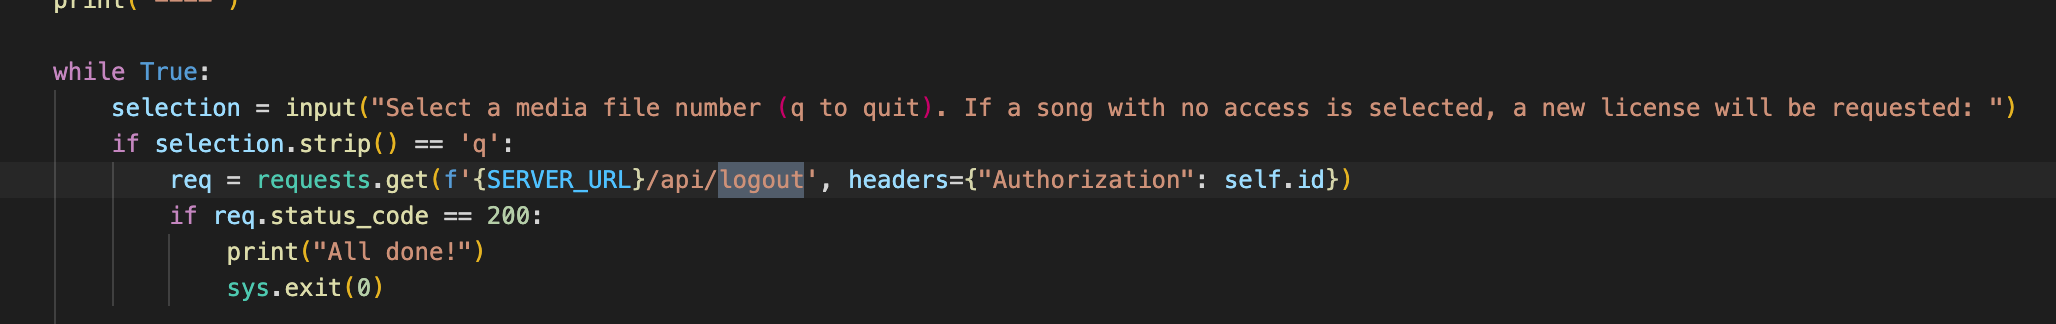
\includegraphics[width=\textwidth]{images/logout_client.png}
        \caption{Envio do pedido de \textit{logout} ao seleccionar a opção de sair da aplicação no cliente}
\end{figure}

\begin{figure}[!h]
        \centering
        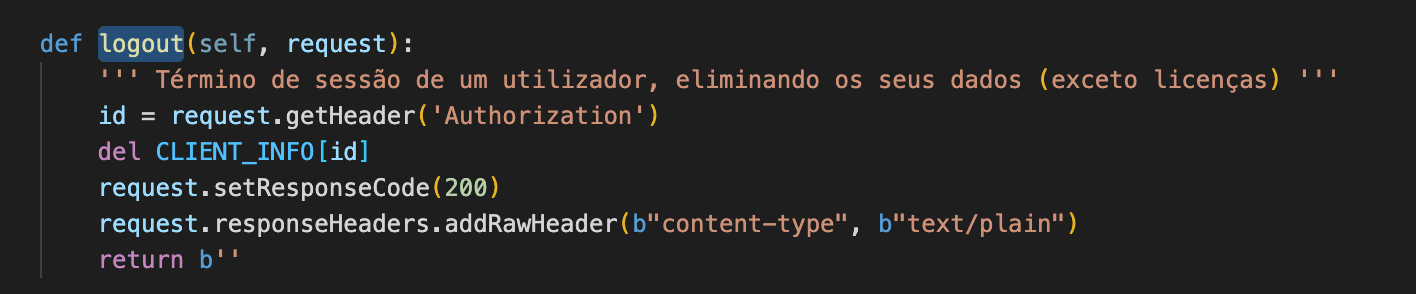
\includegraphics[width=\textwidth]{images/logout_server.png}
        \caption{Informação associada ao cliente eliminada ao receber o pedido de \textit{logout} no servidor}
\end{figure}


\item \textbf{A segunda incide na rotação das chaves} utilizadas na cifra à medida que o cliente obtém novos blocos da música. Para tal, foi utilizada uma solução baseada no algoritmo \textbf{\textit{Double Ratchet}} utilizado em aplicações como o \textit{Signal}. Em suma, o funcionamento deste algoritmo dita que cada mensagem tem de ter uma chave diferente, utilizando para o efeito funções de derivação de chaves, evitando a possibilidade de a partir de uma chave, gerar chaves anteriores devido às propriedades destas funções. Além disso, sempre que possível, deverá fazer-se uma nova troca de chaves utilizando o algoritmo \textit{Diffie-Helman} já abordado anteriormente. Isto é feito para evitar o caso em que alguma chave é interceptada e tem-se acesso à função de derivação, o que permitiria gerar todas as chaves a partir daí.

\par A solução aplicada foi a utilização de uma simples função de síntese aplicada às chaves sempre que se recebe um novo bloco de música e, a cada 5 blocos recebidos, a geração de novas chaves utilizando o algoritmo \textit{Diffie-Helman} mas, utilizando as comunicações cifradas, mantendo todo o secretismo e segurança do início ao fim do programa. A implementação foi a seguinte:

\begin{figure}[!h]
        \centering
        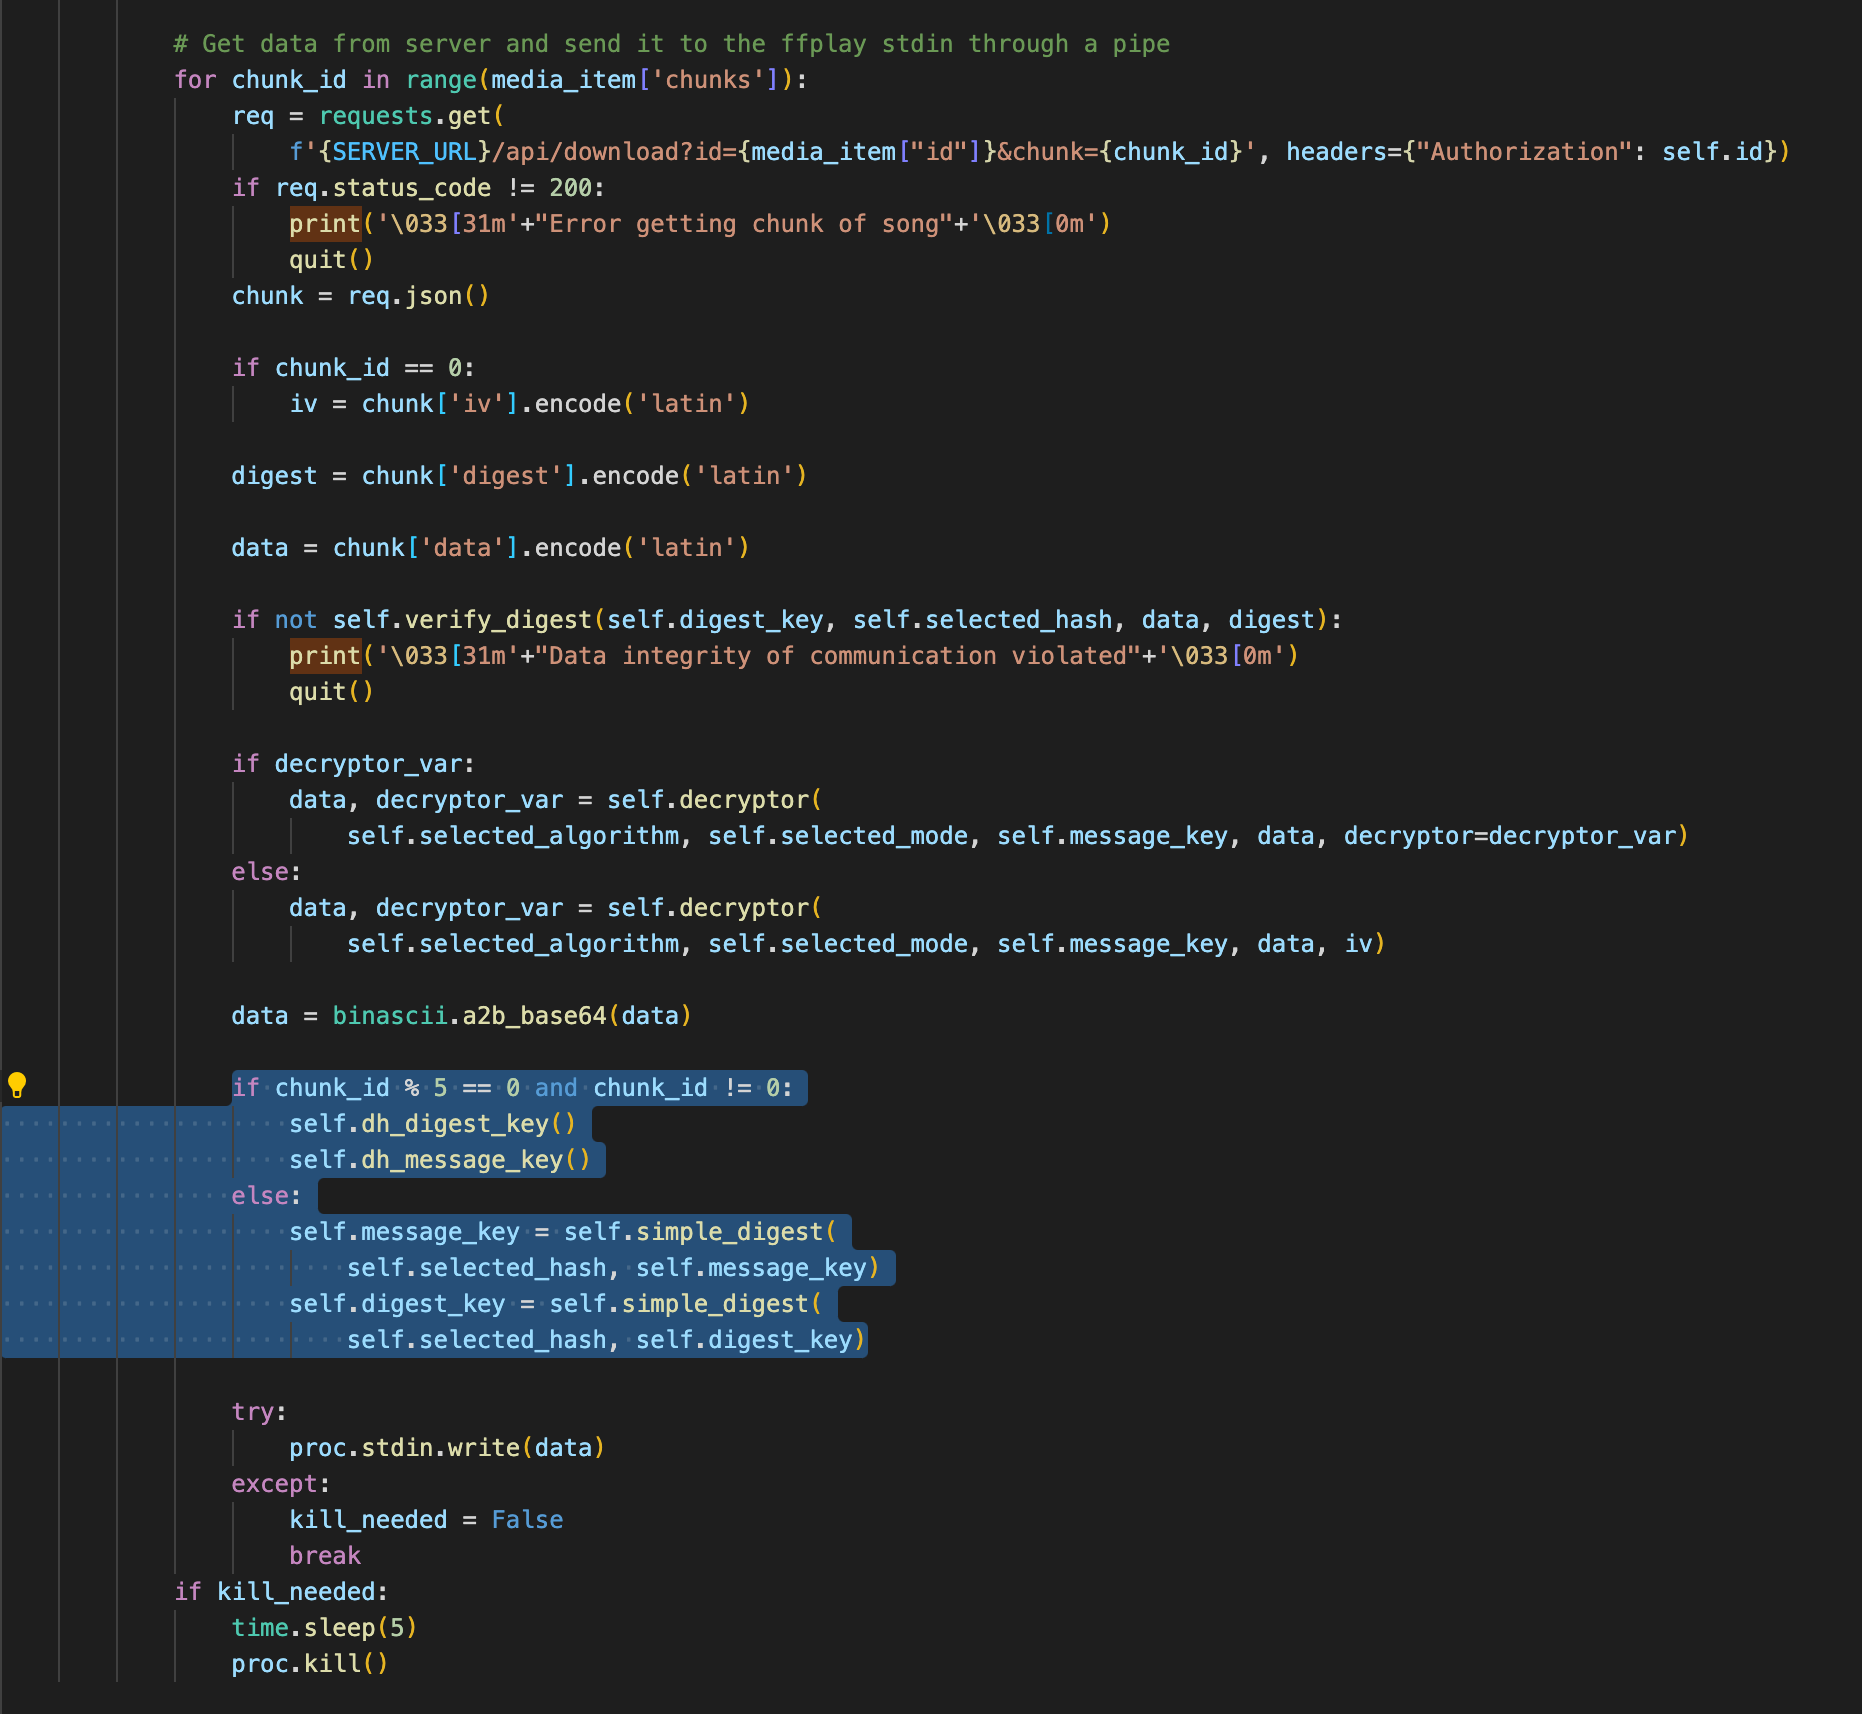
\includegraphics[width=450]{images/download_rotation_client.png}
        \caption{Rotação de chaves (parte assinalada) à medida que se obtém novos blocos de música no cliente}
\end{figure}

\begin{figure}[!h]
        \centering
        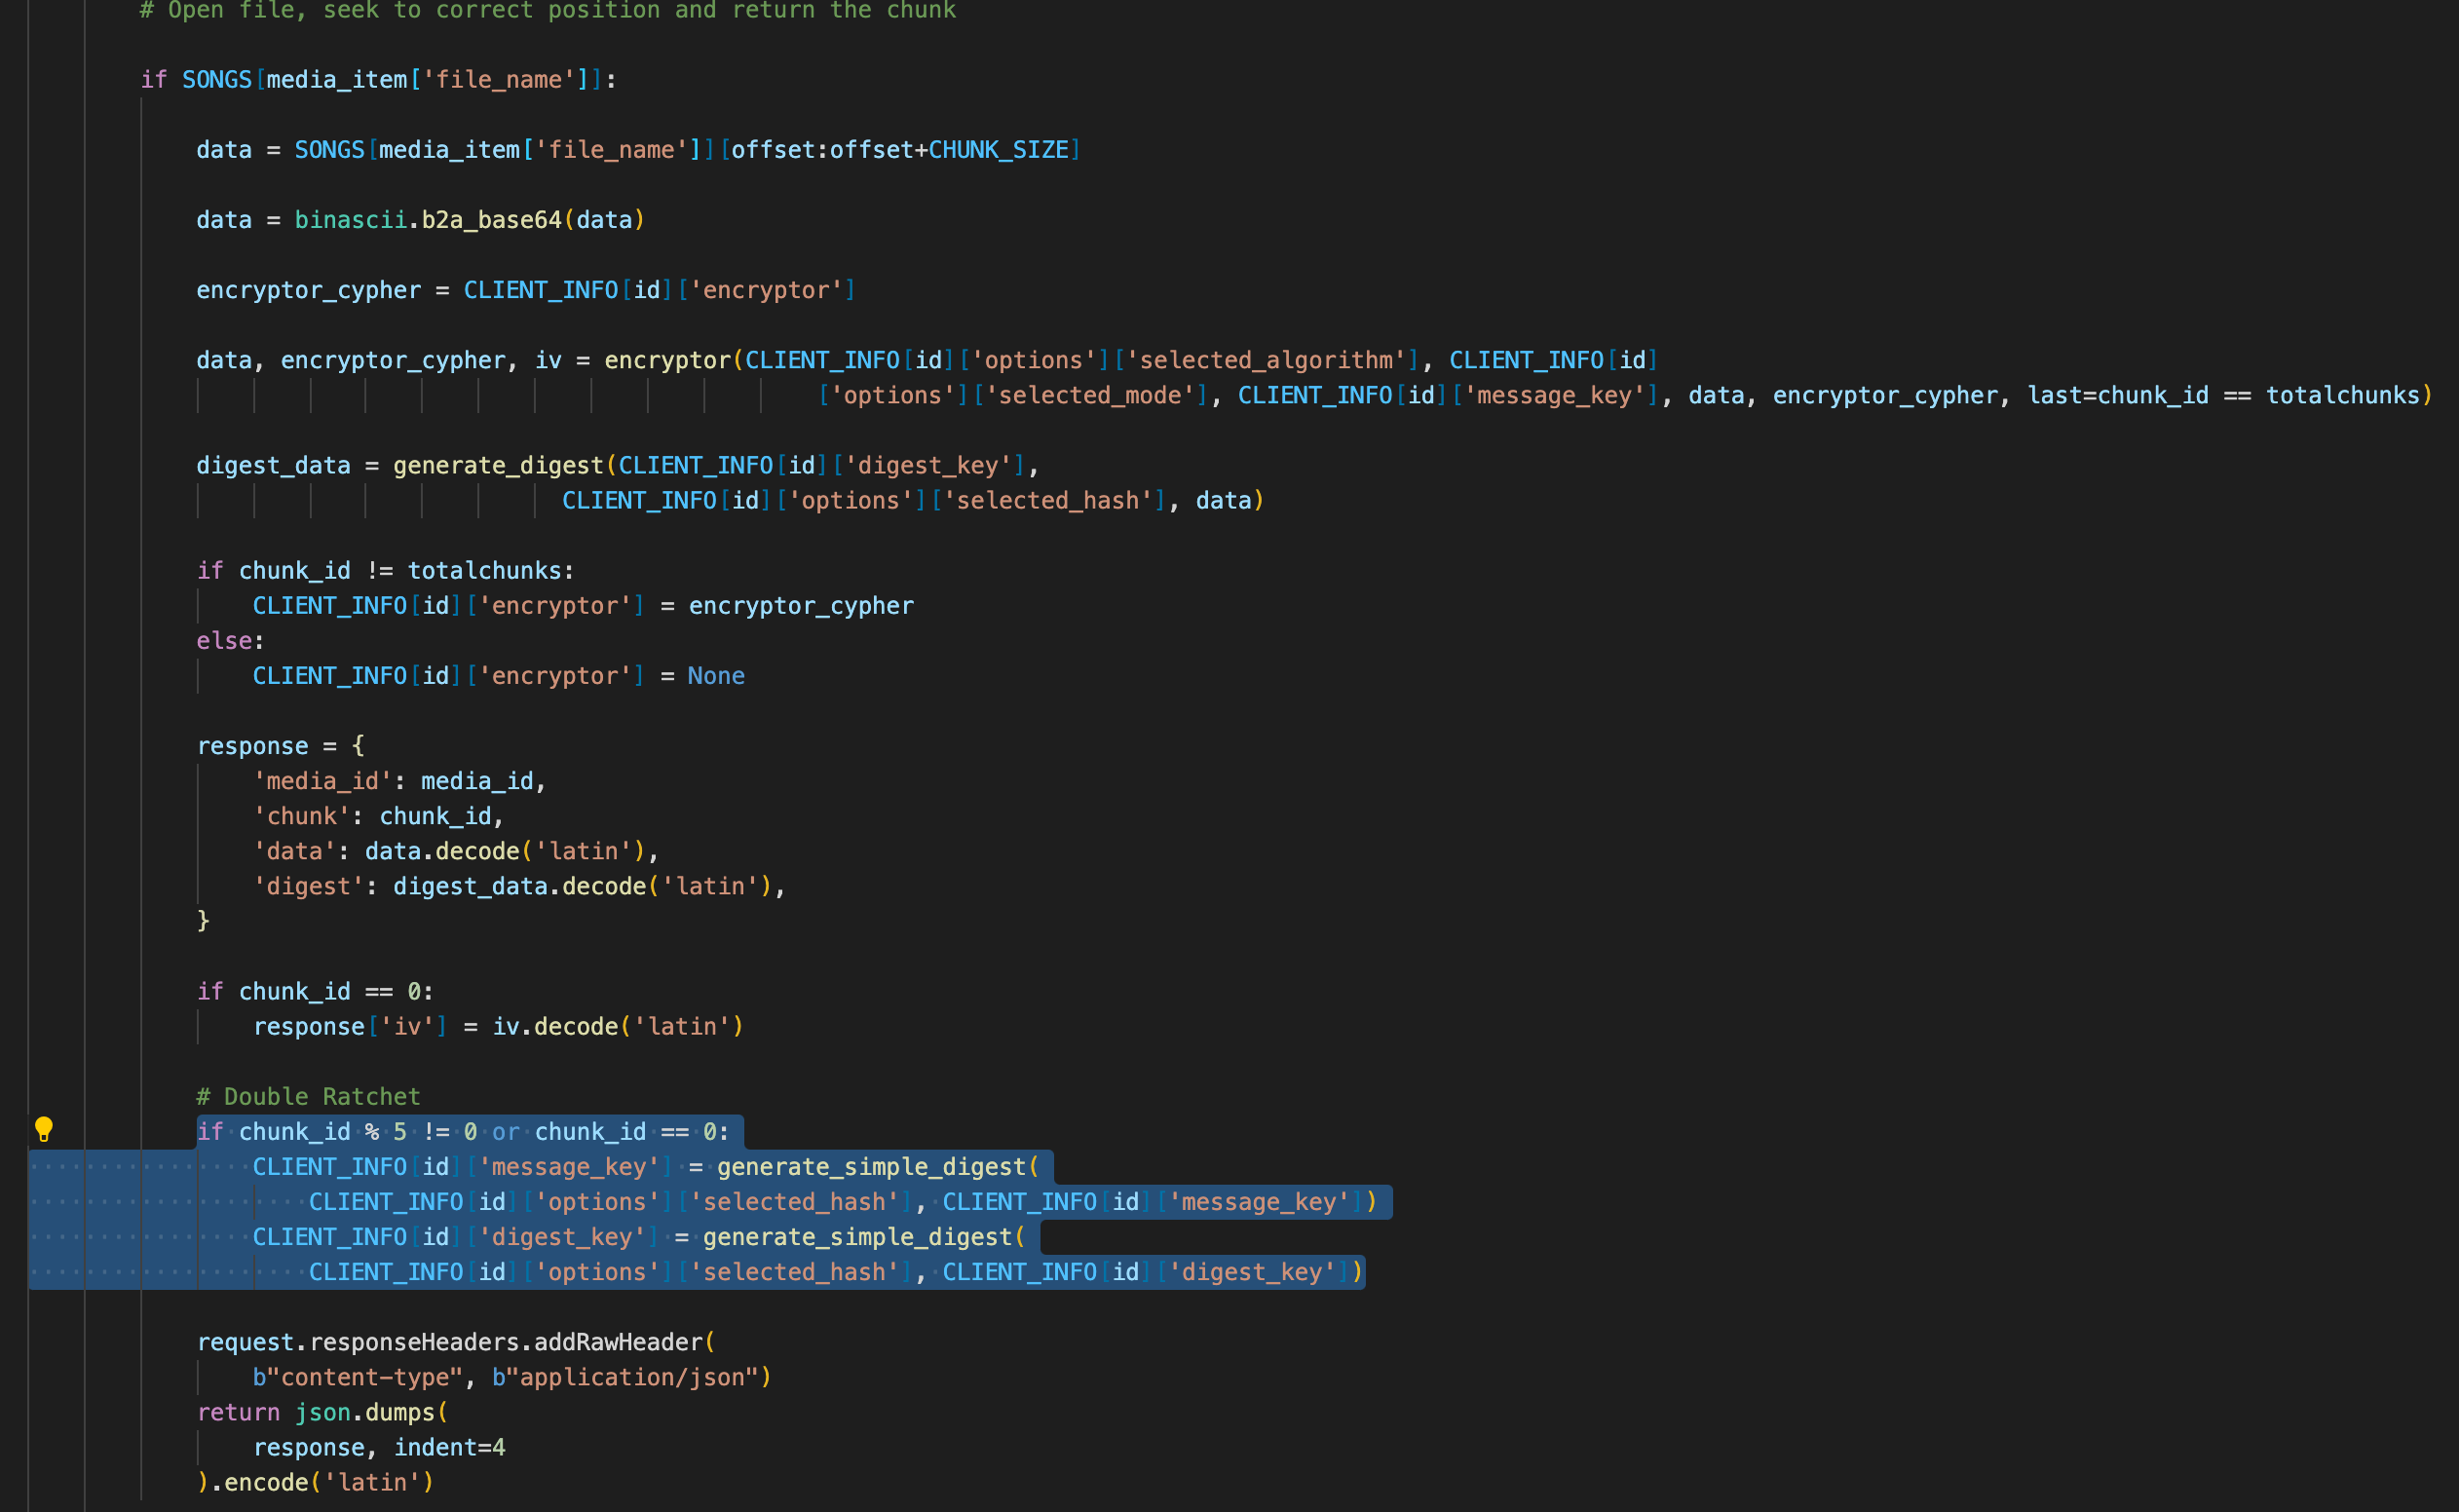
\includegraphics[width=450]{images/download_rotation_server.png}
        \caption{Rotação de chaves (parte assinalada) à medida que se obtém novos blocos de música no servidor}
\end{figure}

\begin{figure}[!h]
        \centering
        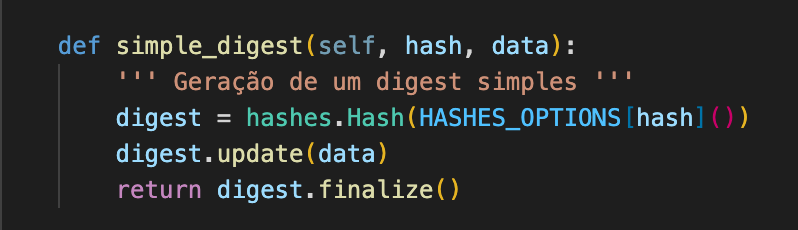
\includegraphics[width=250]{images/simple_digest.png}
        \caption{Função de síntese aplicada às chaves que utiliza o algoritmo de \textit{hash} do protocolo escolhido}
\end{figure}

\end{itemize}

\clearpage

\section{Autenticação e Isolamento}

\subsection{Autenticação do Servidor}

\par Para autenticar o servidor foi criada uma Infraestrutura de chaves públicas personalizada para este caso. A base de dados utilizada no programa \textit{xca} para gerar toda esta Infraestrutura encontra-se na pasta \textit{server\_certs} bem como todos os certificados e chaves privadas geradas para o efeito. Em suma, foi gerado o seguinte:

\begin{itemize}
    \item \textbf{Certificado \textit{Root CA}} desta Infraestrutura
    \item \textbf {Chave privada do Certificado \textit{Root CA}} desta Infraestrutura
     \item \textbf{Certificado do Servidor} assinado pela \textit{Root CA}
     \item \textbf{Chave privada do Certificado do Servidor}
\end{itemize}

\par Com a cifra das comunicações definida e estes certificados gerados, o próximo passo do cliente é autenticar o servidor. Para tal, o cliente faz um pedido ao servidor para obter o certificado do servidor e validar a cadeia de certificação.

\begin{figure}[!h]
        \centering
        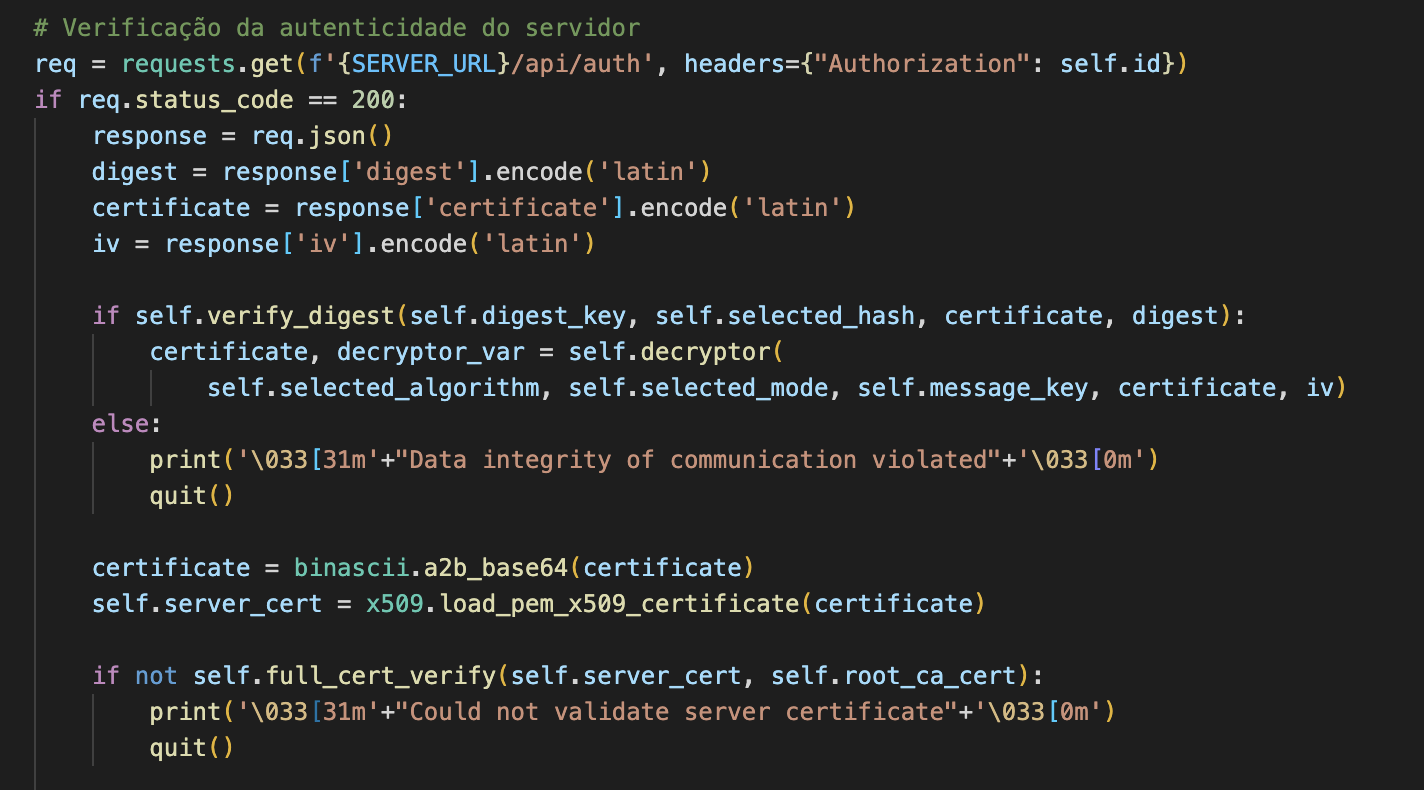
\includegraphics[width=350]{images/server_auth_1_client.png}
        \caption{Pedido do certificado ao servidor e validação no cliente}
\end{figure}

\clearpage

\begin{figure}[!h]
        \centering
        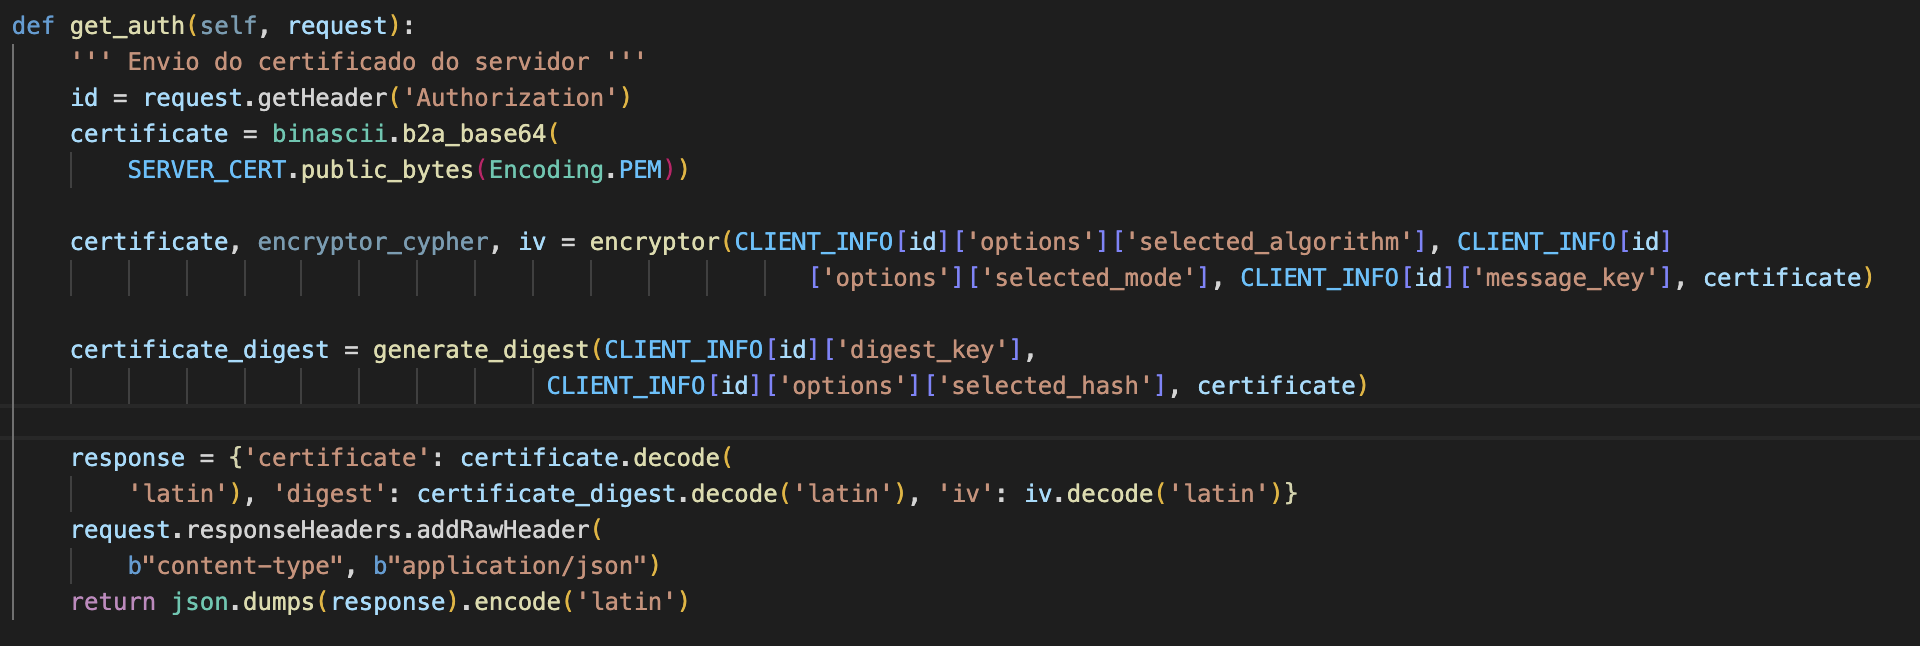
\includegraphics[width=\textwidth]{images/get_auth_server.png}
        \caption{Envio do certificado do servidor, no servidor}
\end{figure}

\par A validação da cadeia de certificação do servidor no cliente apenas utiliza o certificado do servidor e o certificado da entidade emissora, a \textit{Root CA}, carregado ao executar o cliente. Após verificar que o segundo certificado é de uma \textit{Root CA} e é da entidade emissora do certificado do servidor, são verificados três pontos:

\begin{itemize}
    \item \textbf{Validade da data do certificado}
    \item \textbf{Validade da assinatura do certificado}
    \item \textbf{Validade dos \textit{purposes}} - Neste caso verificando se o objetivo do certificado é para \textit{TLS Web Server Authentication}
\end{itemize}

\par Escolheu-se, para esta Infraestrutura, não se criar listas de revogação de certificados, uma vez que não acrescentariam grandes benefícios e o funcionamento destas seriam testadas com a integração de um \textit{hardware token}. A implementação do processo descrito é a seguinte:

\begin{figure}[!h]
        \centering
        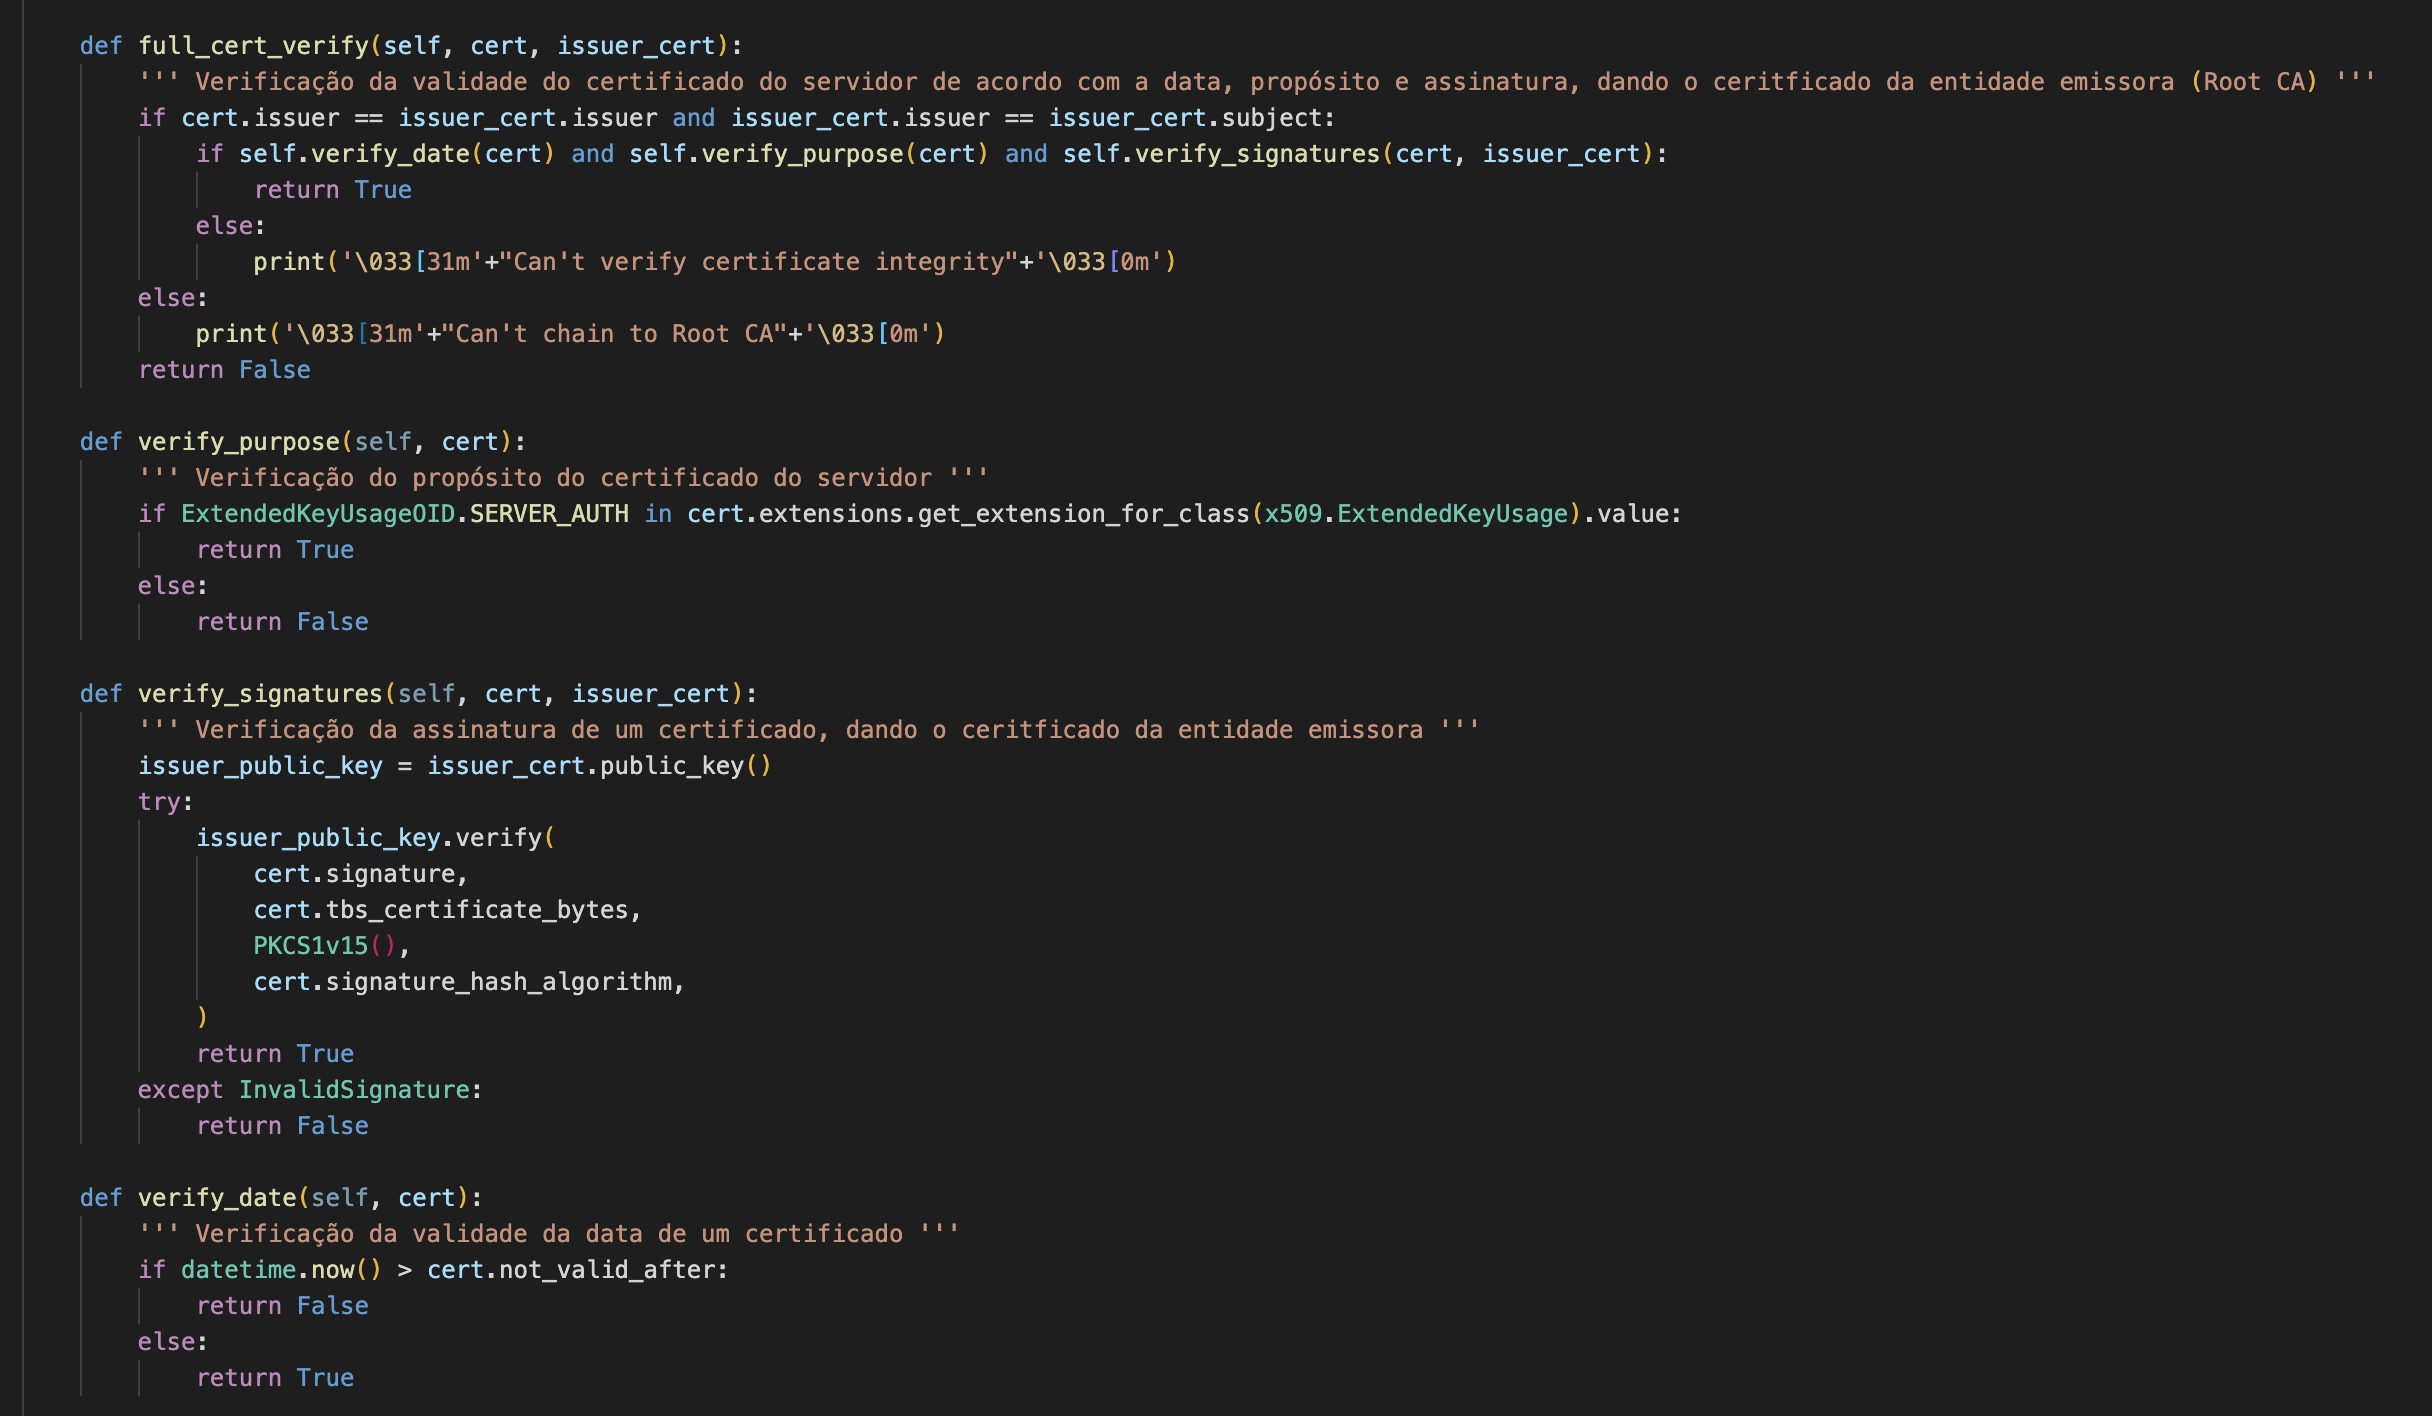
\includegraphics[width=\textwidth]{images/cert_validation_client.png}
        \caption{Processo de validação da cadeia de certificação do certificado do servidor, no cliente}
\end{figure}

\clearpage

\par Para o resto da autenticação do servidor recorreu-se ao conjunto de protocolos de segurança de comunicações, \textbf{Autenticação Desafio-Resposta}, abordado nas aulas teóricas. No fundo, o funcionamento assenta no envio de um \textbf{Desafio} por uma entidade, sendo que a outra entidade terá de enviar uma \textbf{Resposta Válida} para se autenticar.

\par Utilizando a Autenticação Desafio-Resposta, a autenticação do servidor é terminada com o envio de uma \textit{nounce}, um número arbitrário apenas utilizado uma vez, por parte do cliente, representando o \textbf{Desafio}, e o servidor por sua vez responde com essa \textit{nounce} assinada com a sua chave privada, de modo a que esta assinatura seja validada por parte do cliente, autenticando o servidor:

\begin{figure}[!h]
        \centering
        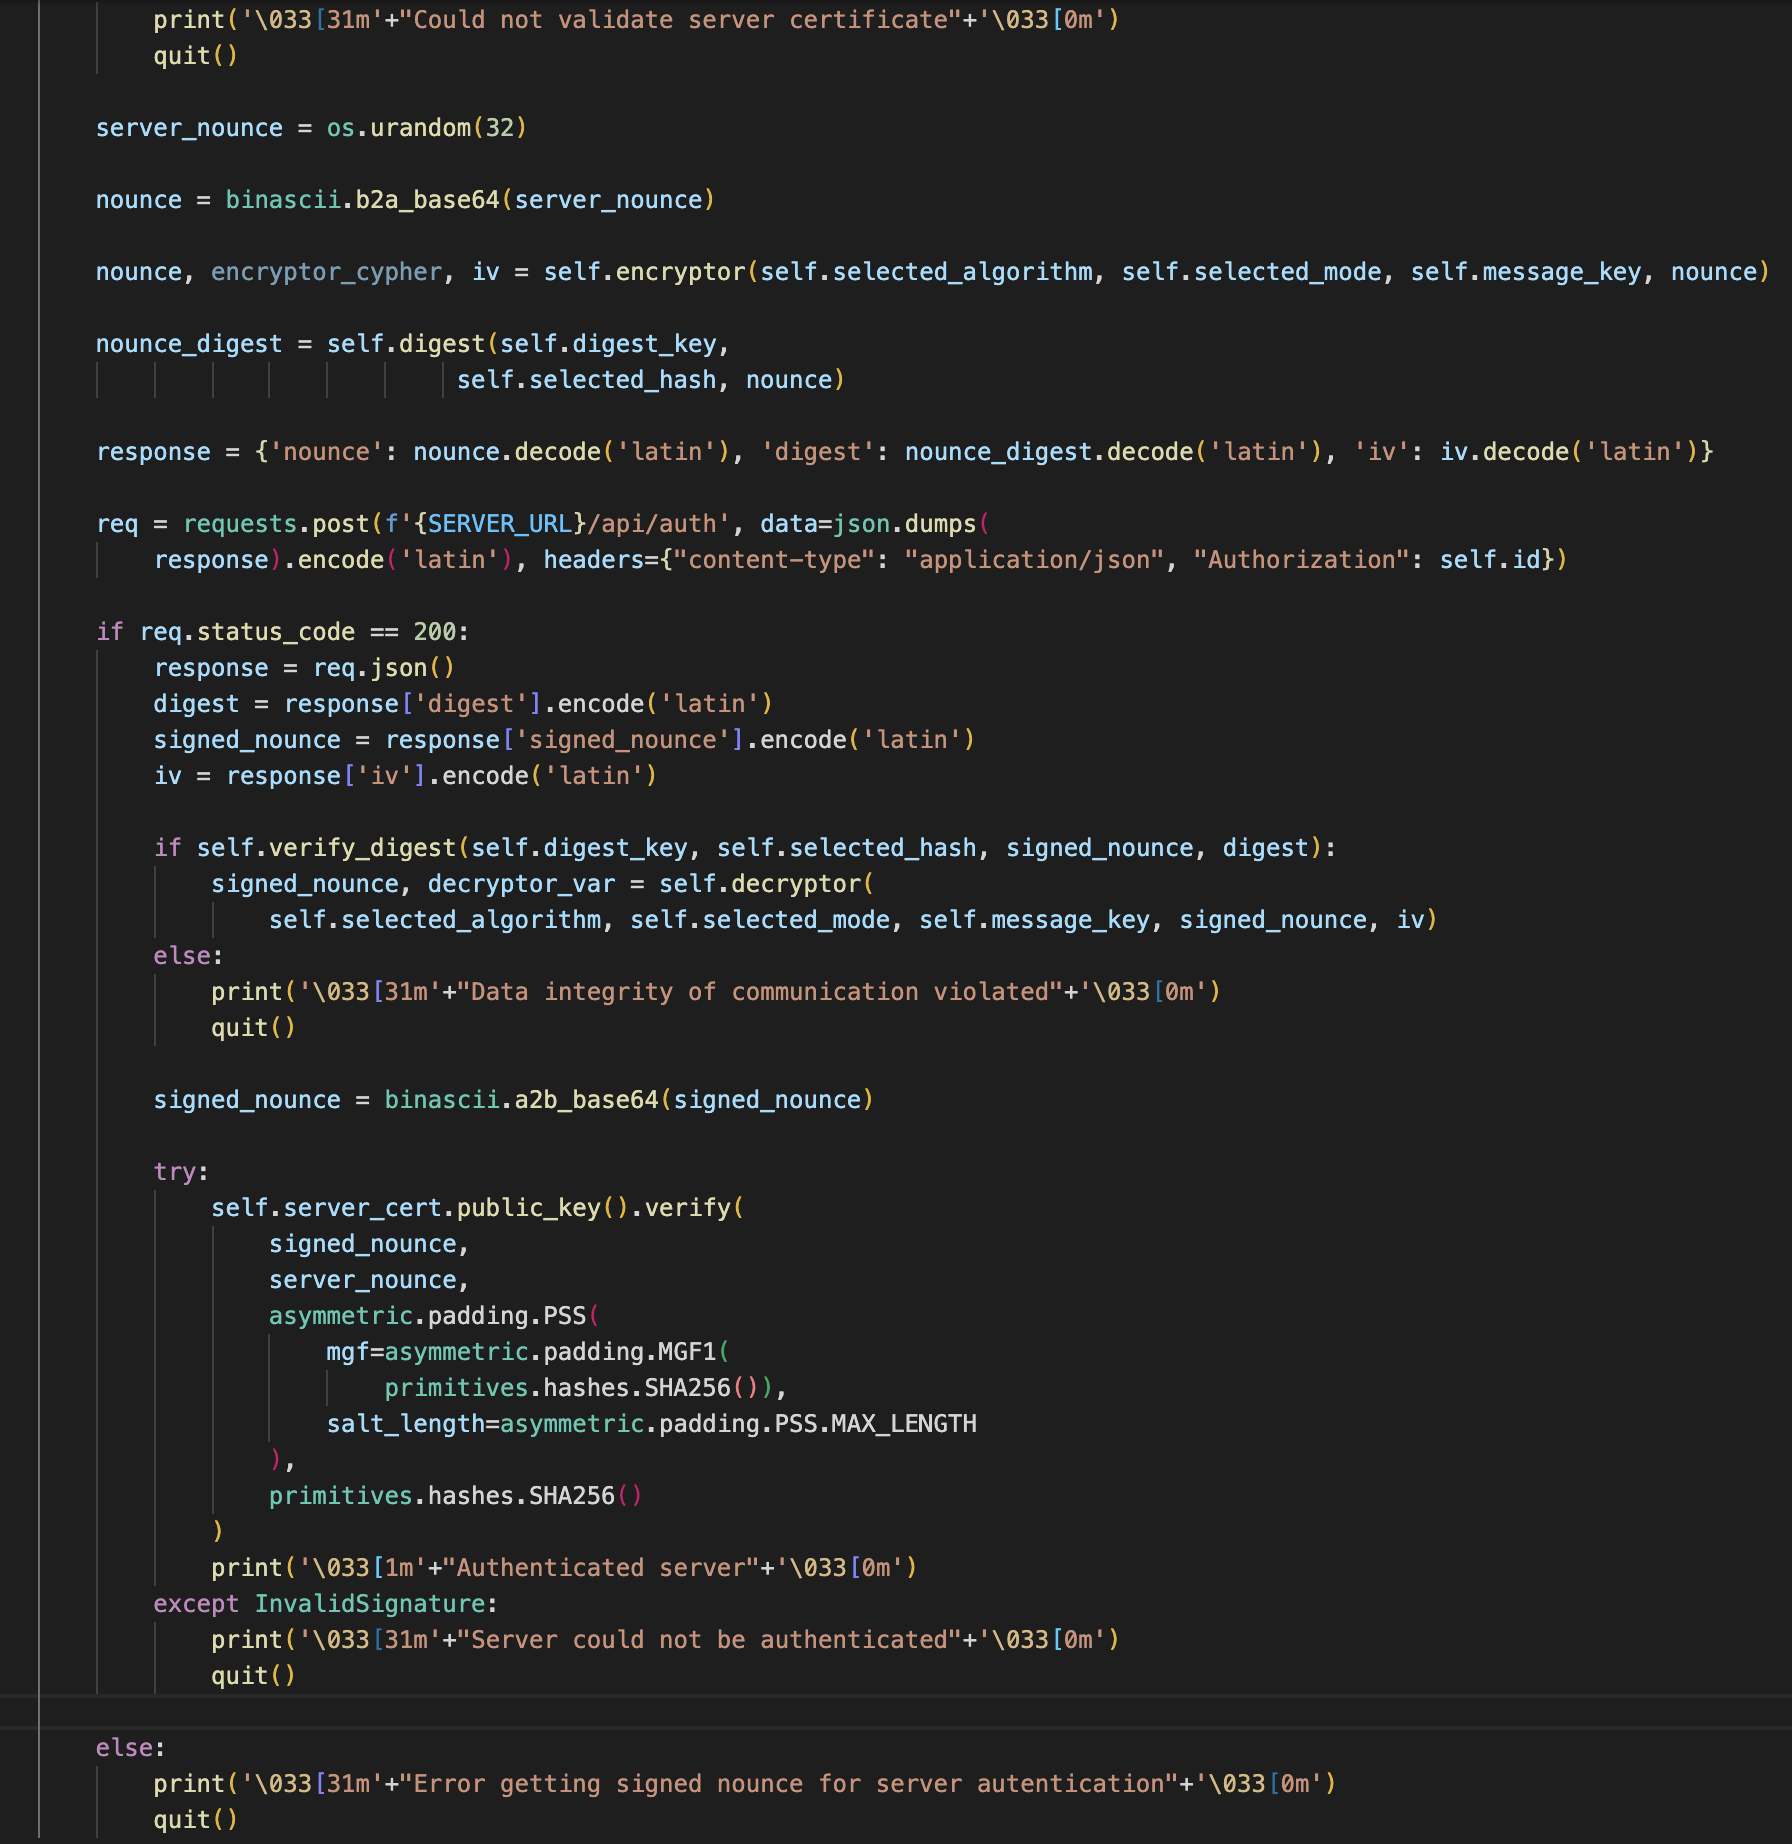
\includegraphics[width=400]{images/server_auth_2_client.png}
        \caption{Autenticação Desafio-Resposta aplicada no final da autenticação do servidor, no cliente}
\end{figure}

\begin{figure}[!h]
        \centering
        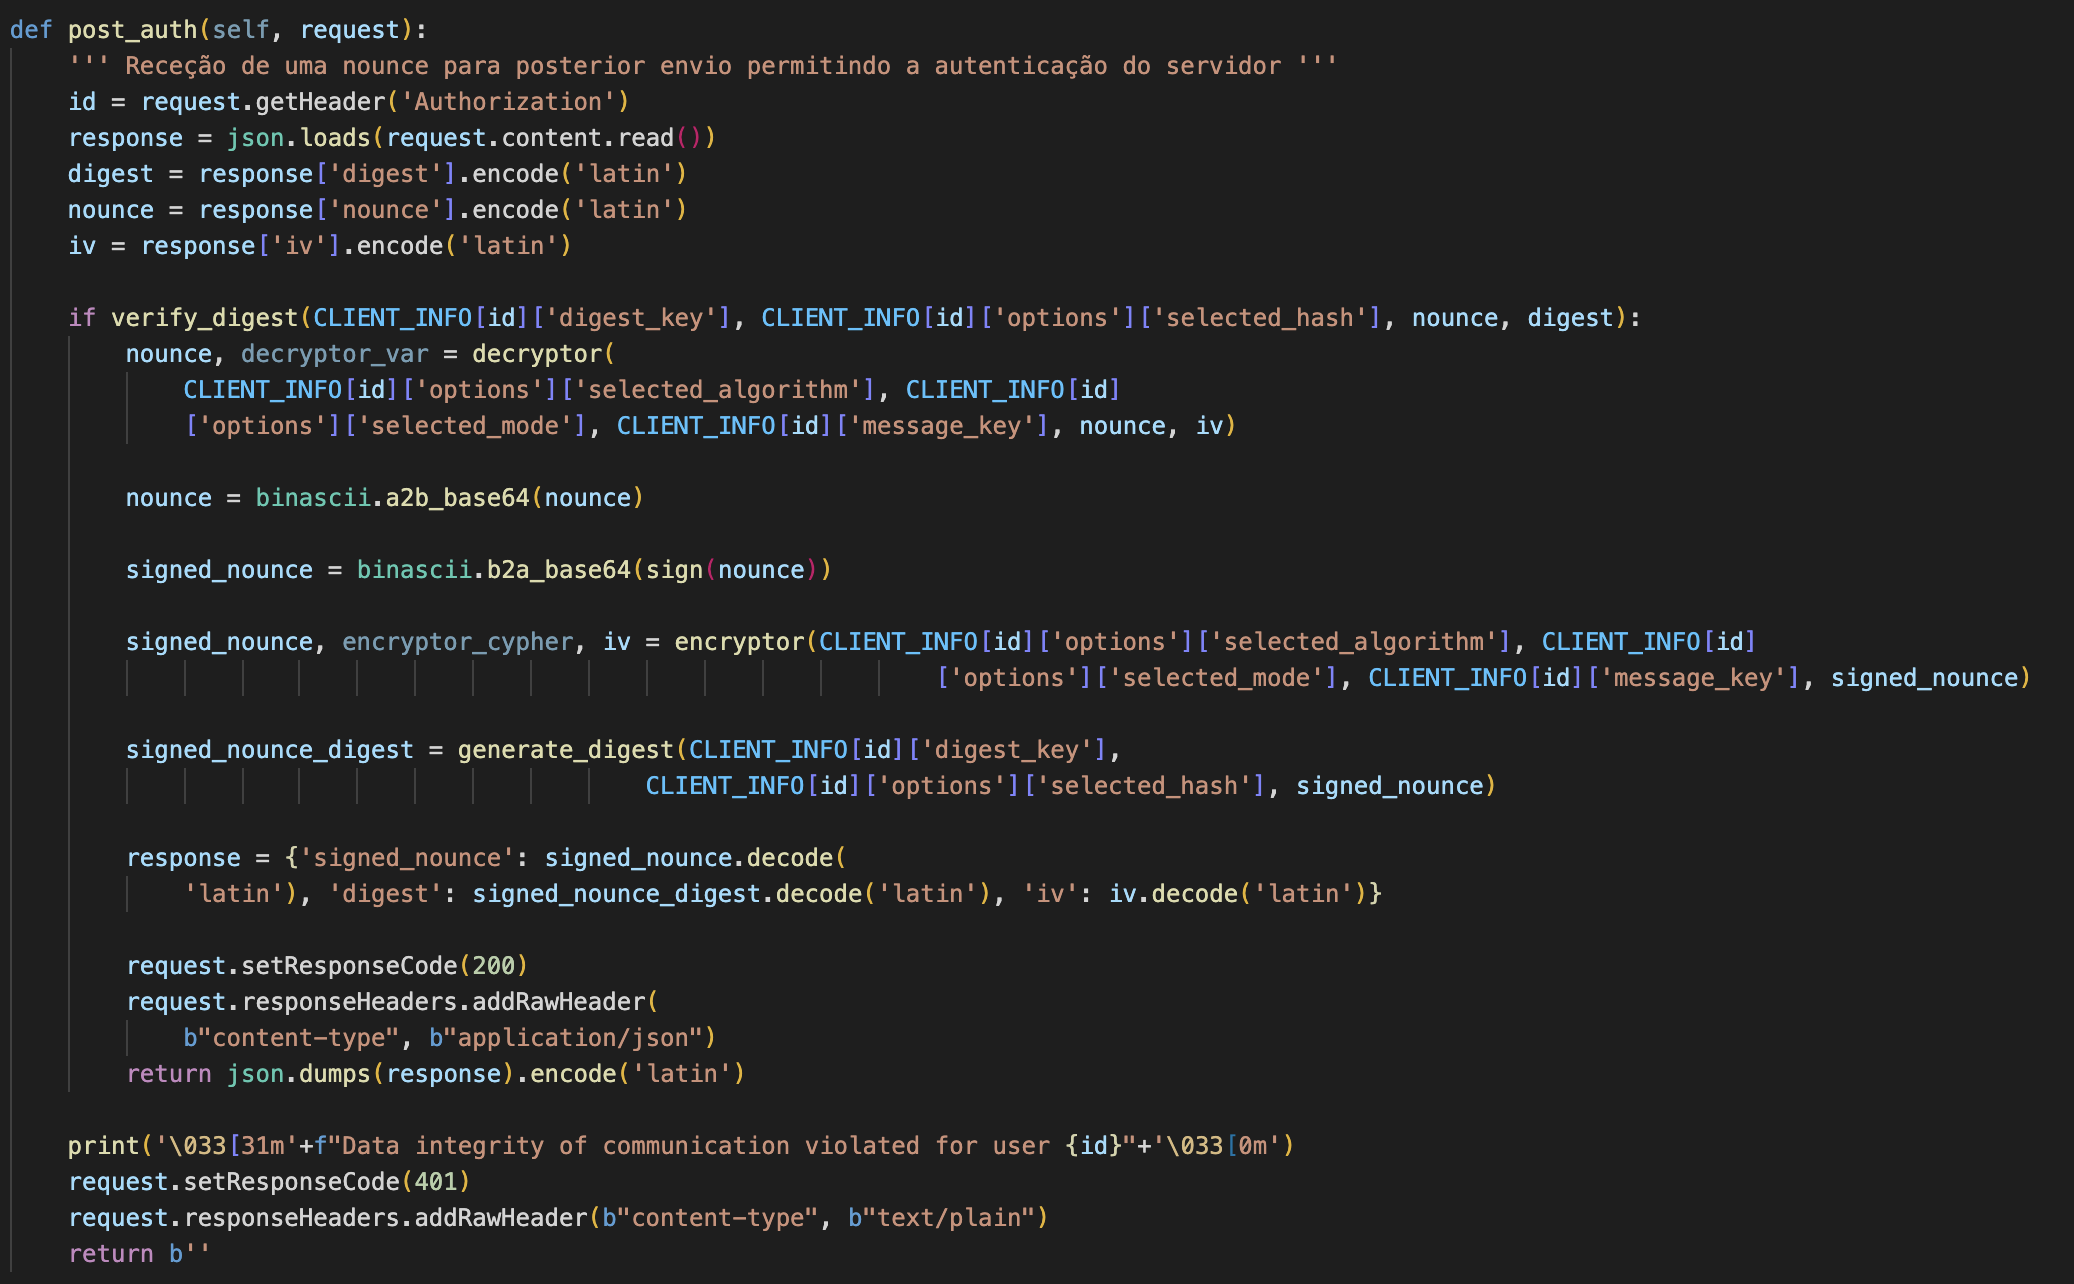
\includegraphics[width=400]{images/post_auth_server.png}
        \caption{Reposta do pedido de assinatura da \textit{nounce} para a Autenticação Desafio-Resposta aplicada no final da autenticação do servidor, no servidor}
\end{figure}

\begin{figure}[!h]
        \centering
        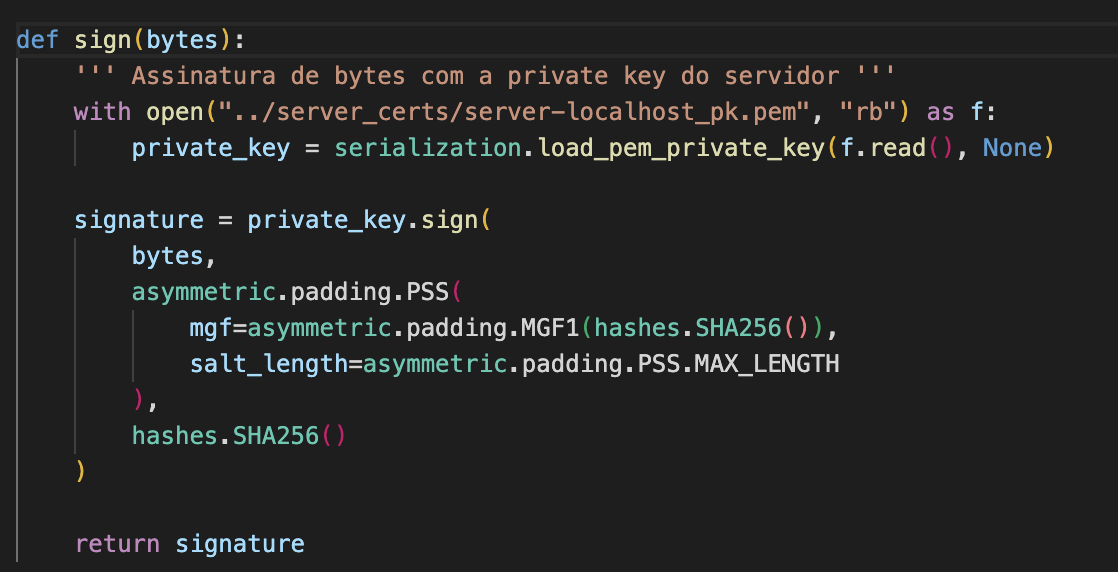
\includegraphics[width=300]{images/sign_server.png}
        \caption{Função de assinatura de dados com a chave privada do servidor, no servidor}
\end{figure}

\clearpage

\subsection{Autenticação do Cliente}

\par Para o servidor autenticar o cliente, escolheu-se utilizar um \textit{hardware token}, o cartão de cidadão. Ao iniciar a aplicação do cliente é verificada a presença de um cartão de cidadão e, caso esteja presente, é feito o carregamento inicial de diversos dados usados posteriormente. Isto tudo acontece na função \textit{get\_cc}:

\begin{figure}[!h]
        \centering
        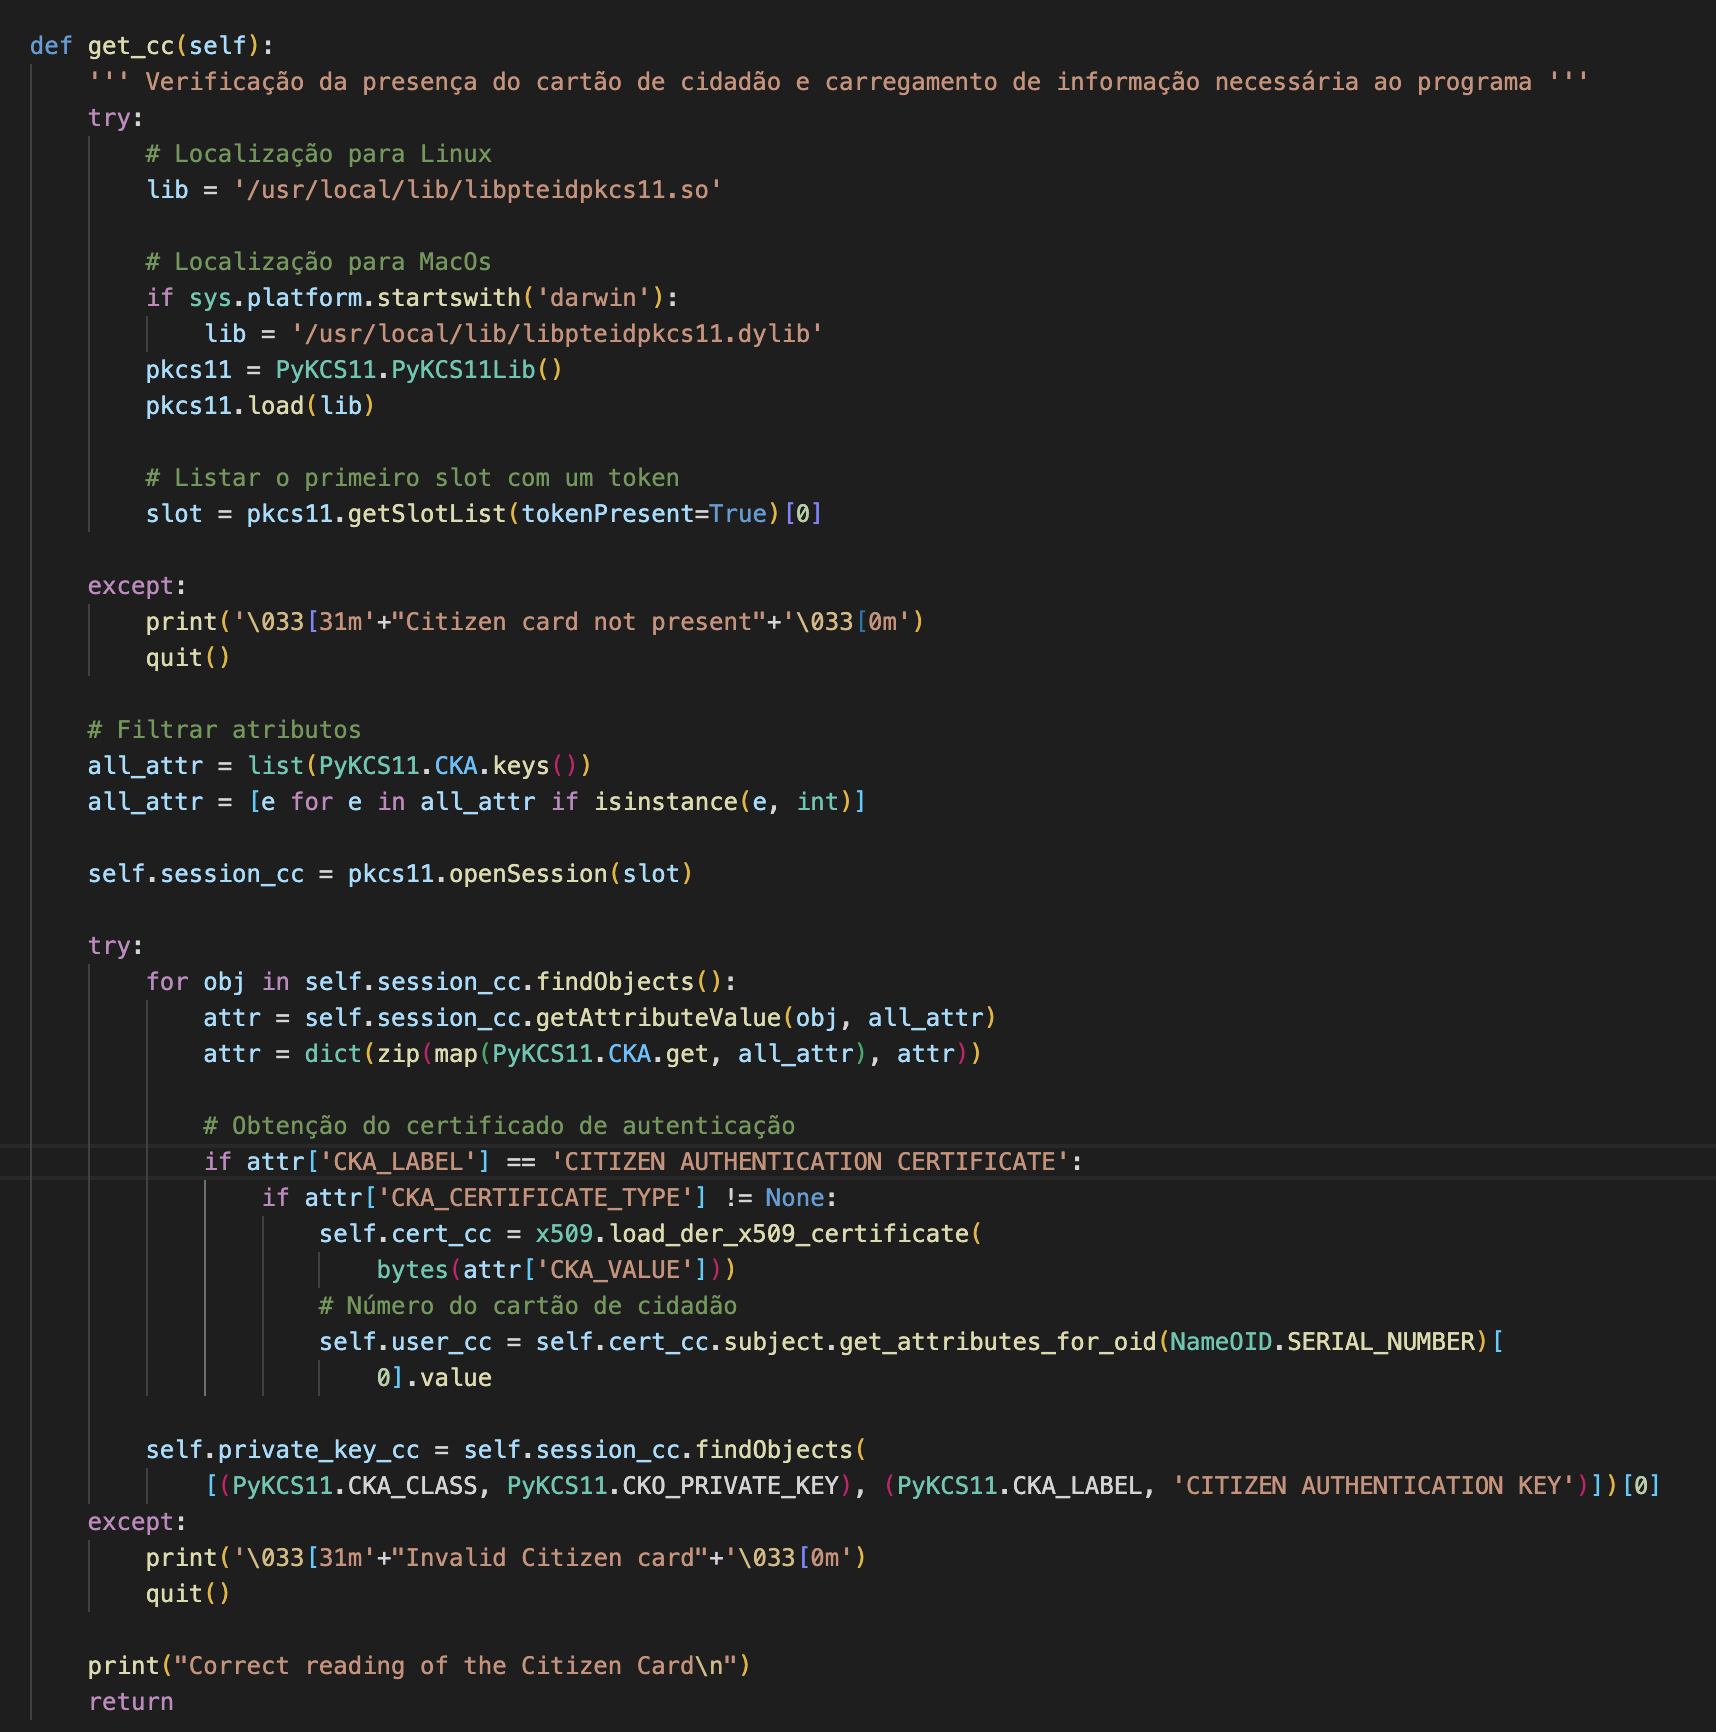
\includegraphics[width=450]{images/get_cc_client.png}
        \caption{Leitura inicial do cartão de cidadão por parte do cliente}
\end{figure}

\par É guardado em memória o certificado relativo ao cartão de cidadão, a sessão, a chave privada e o número do cartão.

\clearpage

\par Com isto feito, já depois da autenticação do servidor, volta-se a utilizar a Autenticação Desafio-Resposta, referida anteriormente, para o servidor validar o cliente. Para tal, é feito um pedido ao servidor de modo a obter uma \textit{nounce} gerada pelo mesmo, sendo esta assinada com a chave privada do cartão de cidadão no cliente, colocando-se as credenciais necessárias para tal. Com a \textit{nounce} assinada, é enviado ao servidor o certificado do cartão de cidadão e a \textit{nounce} assinada de modo a permitir a autenticação do cliente.

\begin{figure}[!h]
        \centering
        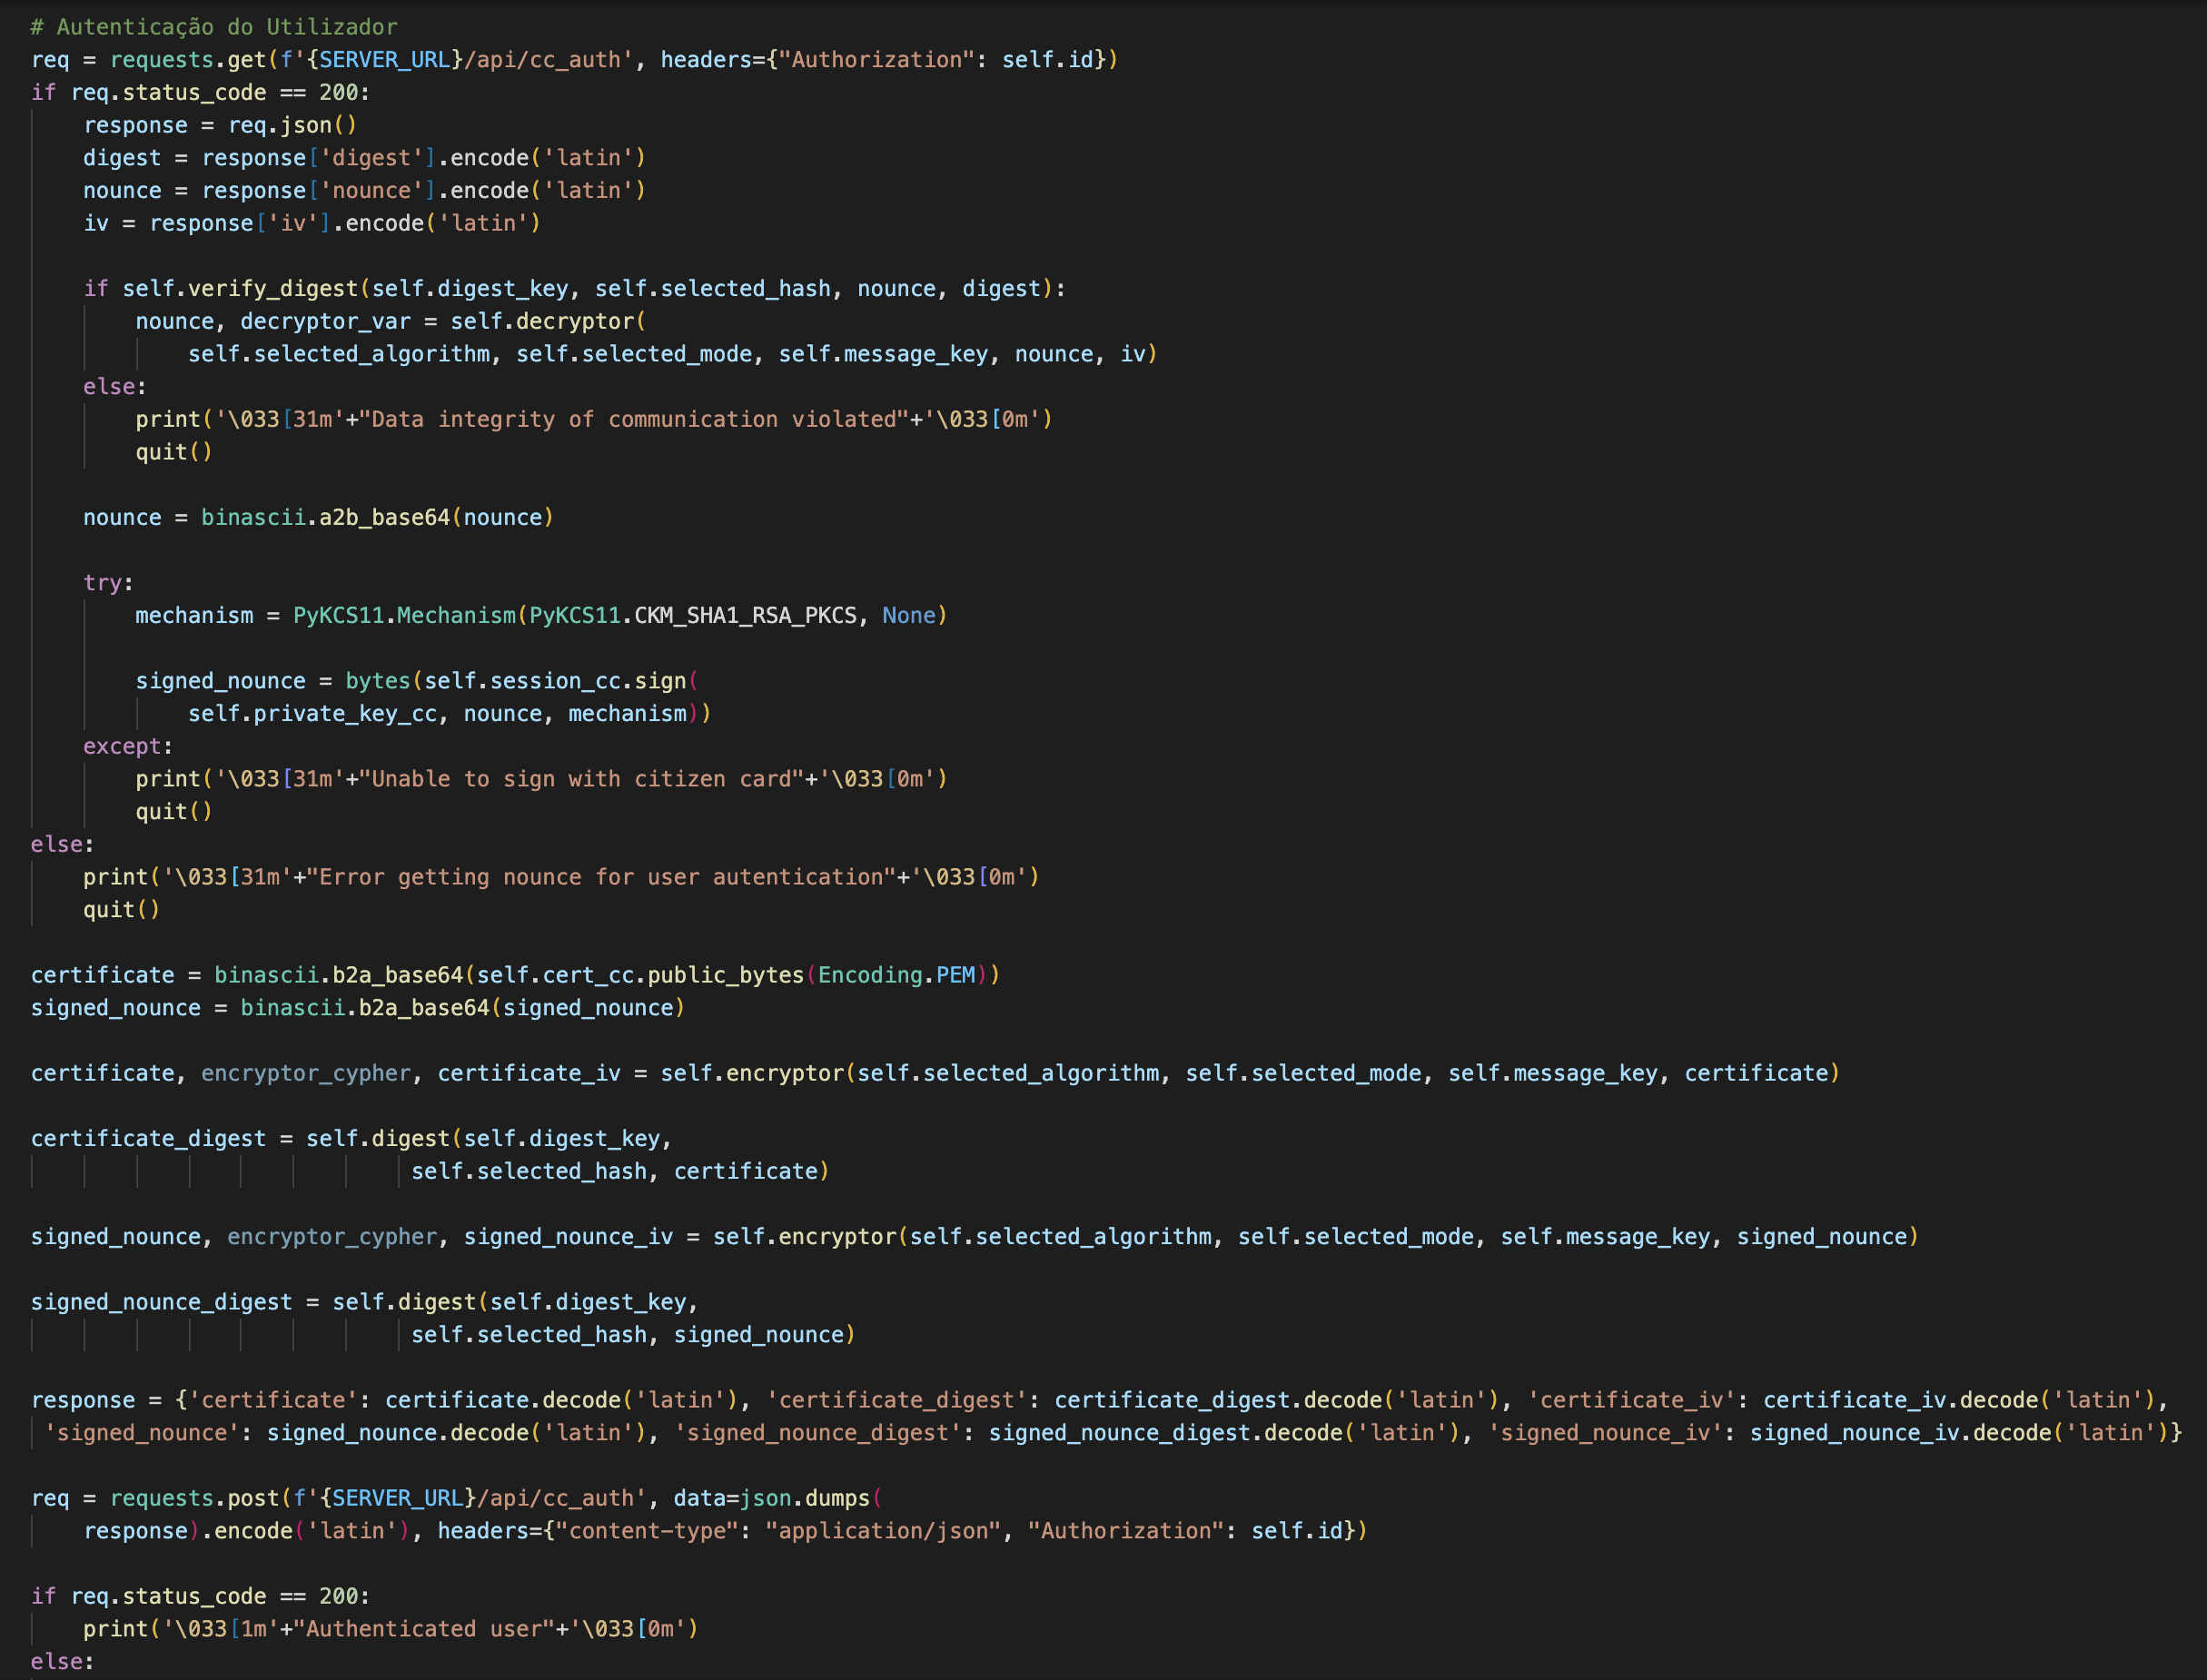
\includegraphics[width=\textwidth]{images/cc_auth_client.png}
        \caption{Processo de autenticação do cliente, no cliente}
\end{figure}

\clearpage

\par Para validar a cadeia de certificação do certificado do cartão de cidadão, o servidor, ao inicializar, necessita de carregar certificados intermédios e de raiz, bem como listas de revogação do governo e de outras entidades utilizadas para validar estes certificados. Para tal, foram utilizadas as funções \textit{get\_chain} e \textit{get\_crls}, sendo que a primeira tem a responsabilidade de carregar os certificados intermédios e de raiz e a segunda tem a responsabilidade de carregar as listas de revogação, previamente obtidas nos endereços presentes na Bibliografia. De notar que, devido ao trabalho ter sido testado em \textit{MacOS} e os certificados raiz, neste SO, serem guardados de maneira diferente, optou-se ao invés de carregar os certificados na localização \textit{/etc/ssl/certs}, como habitualmente, carregar o certificado raiz da cadeia de certificação do cartão de cidadão utilizado, guardado previamente.

\begin{figure}[!h]
        \centering
        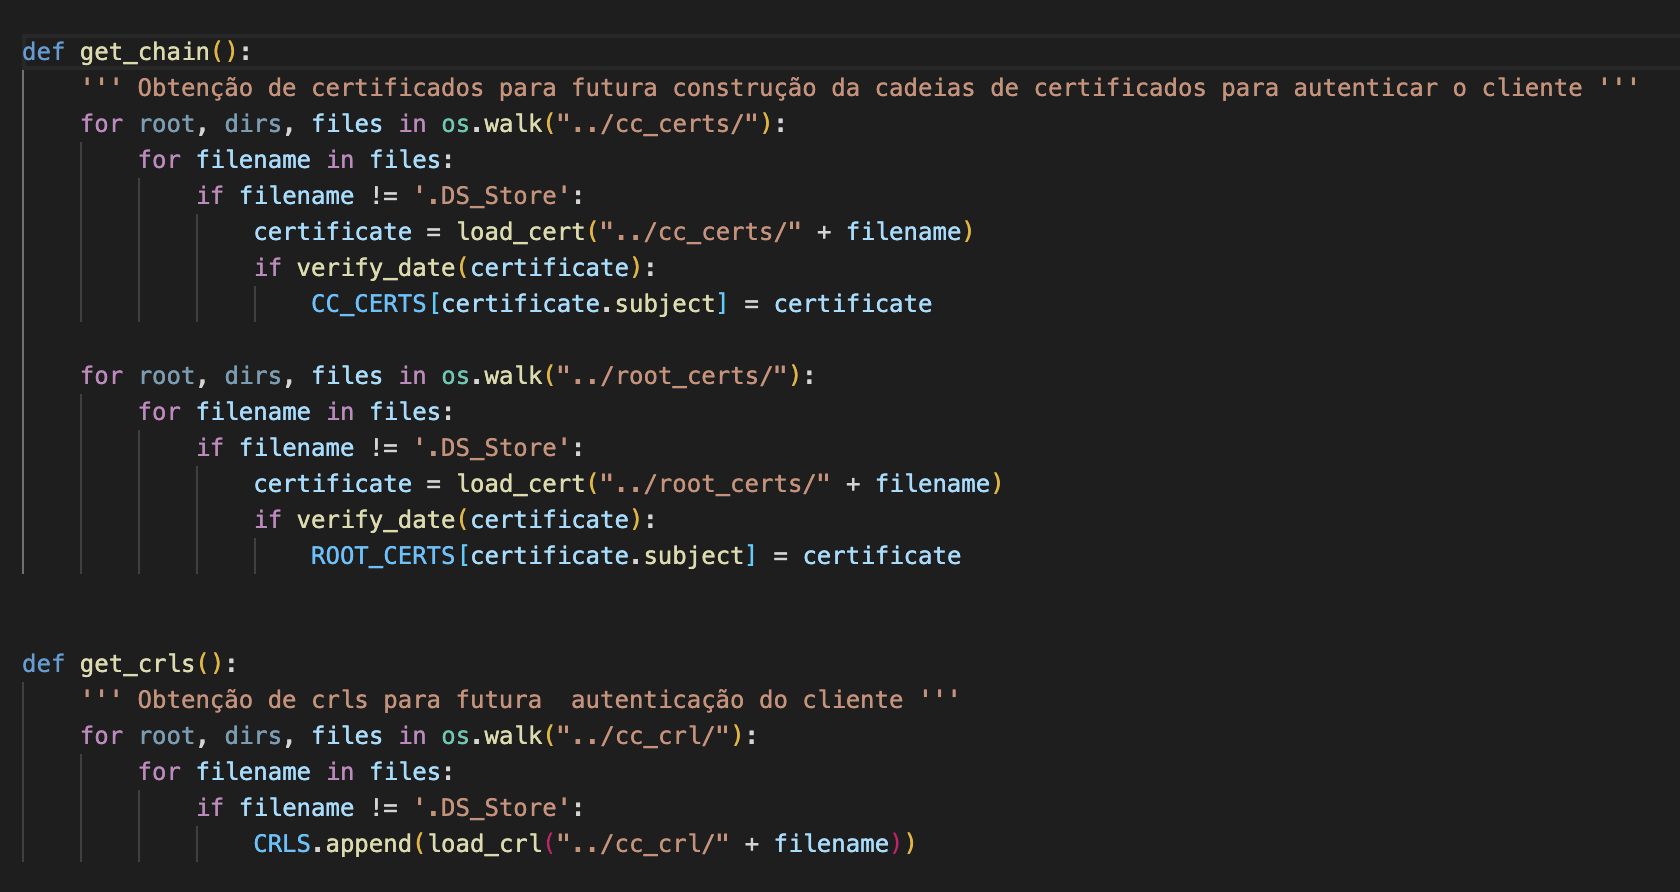
\includegraphics[width=\textwidth]{images/get_chain_get_crl.png}
        \caption{Processo carregamento dos certificados intermédia, raiz e listas de revogação no servidor}
\end{figure}

\clearpage

\par Com toda esta informação carregada previamente, é possível validar a cadeia de certificação do certificado recebido e validar a \textit{nounce} assinada:

\begin{figure}[!h]
        \centering
        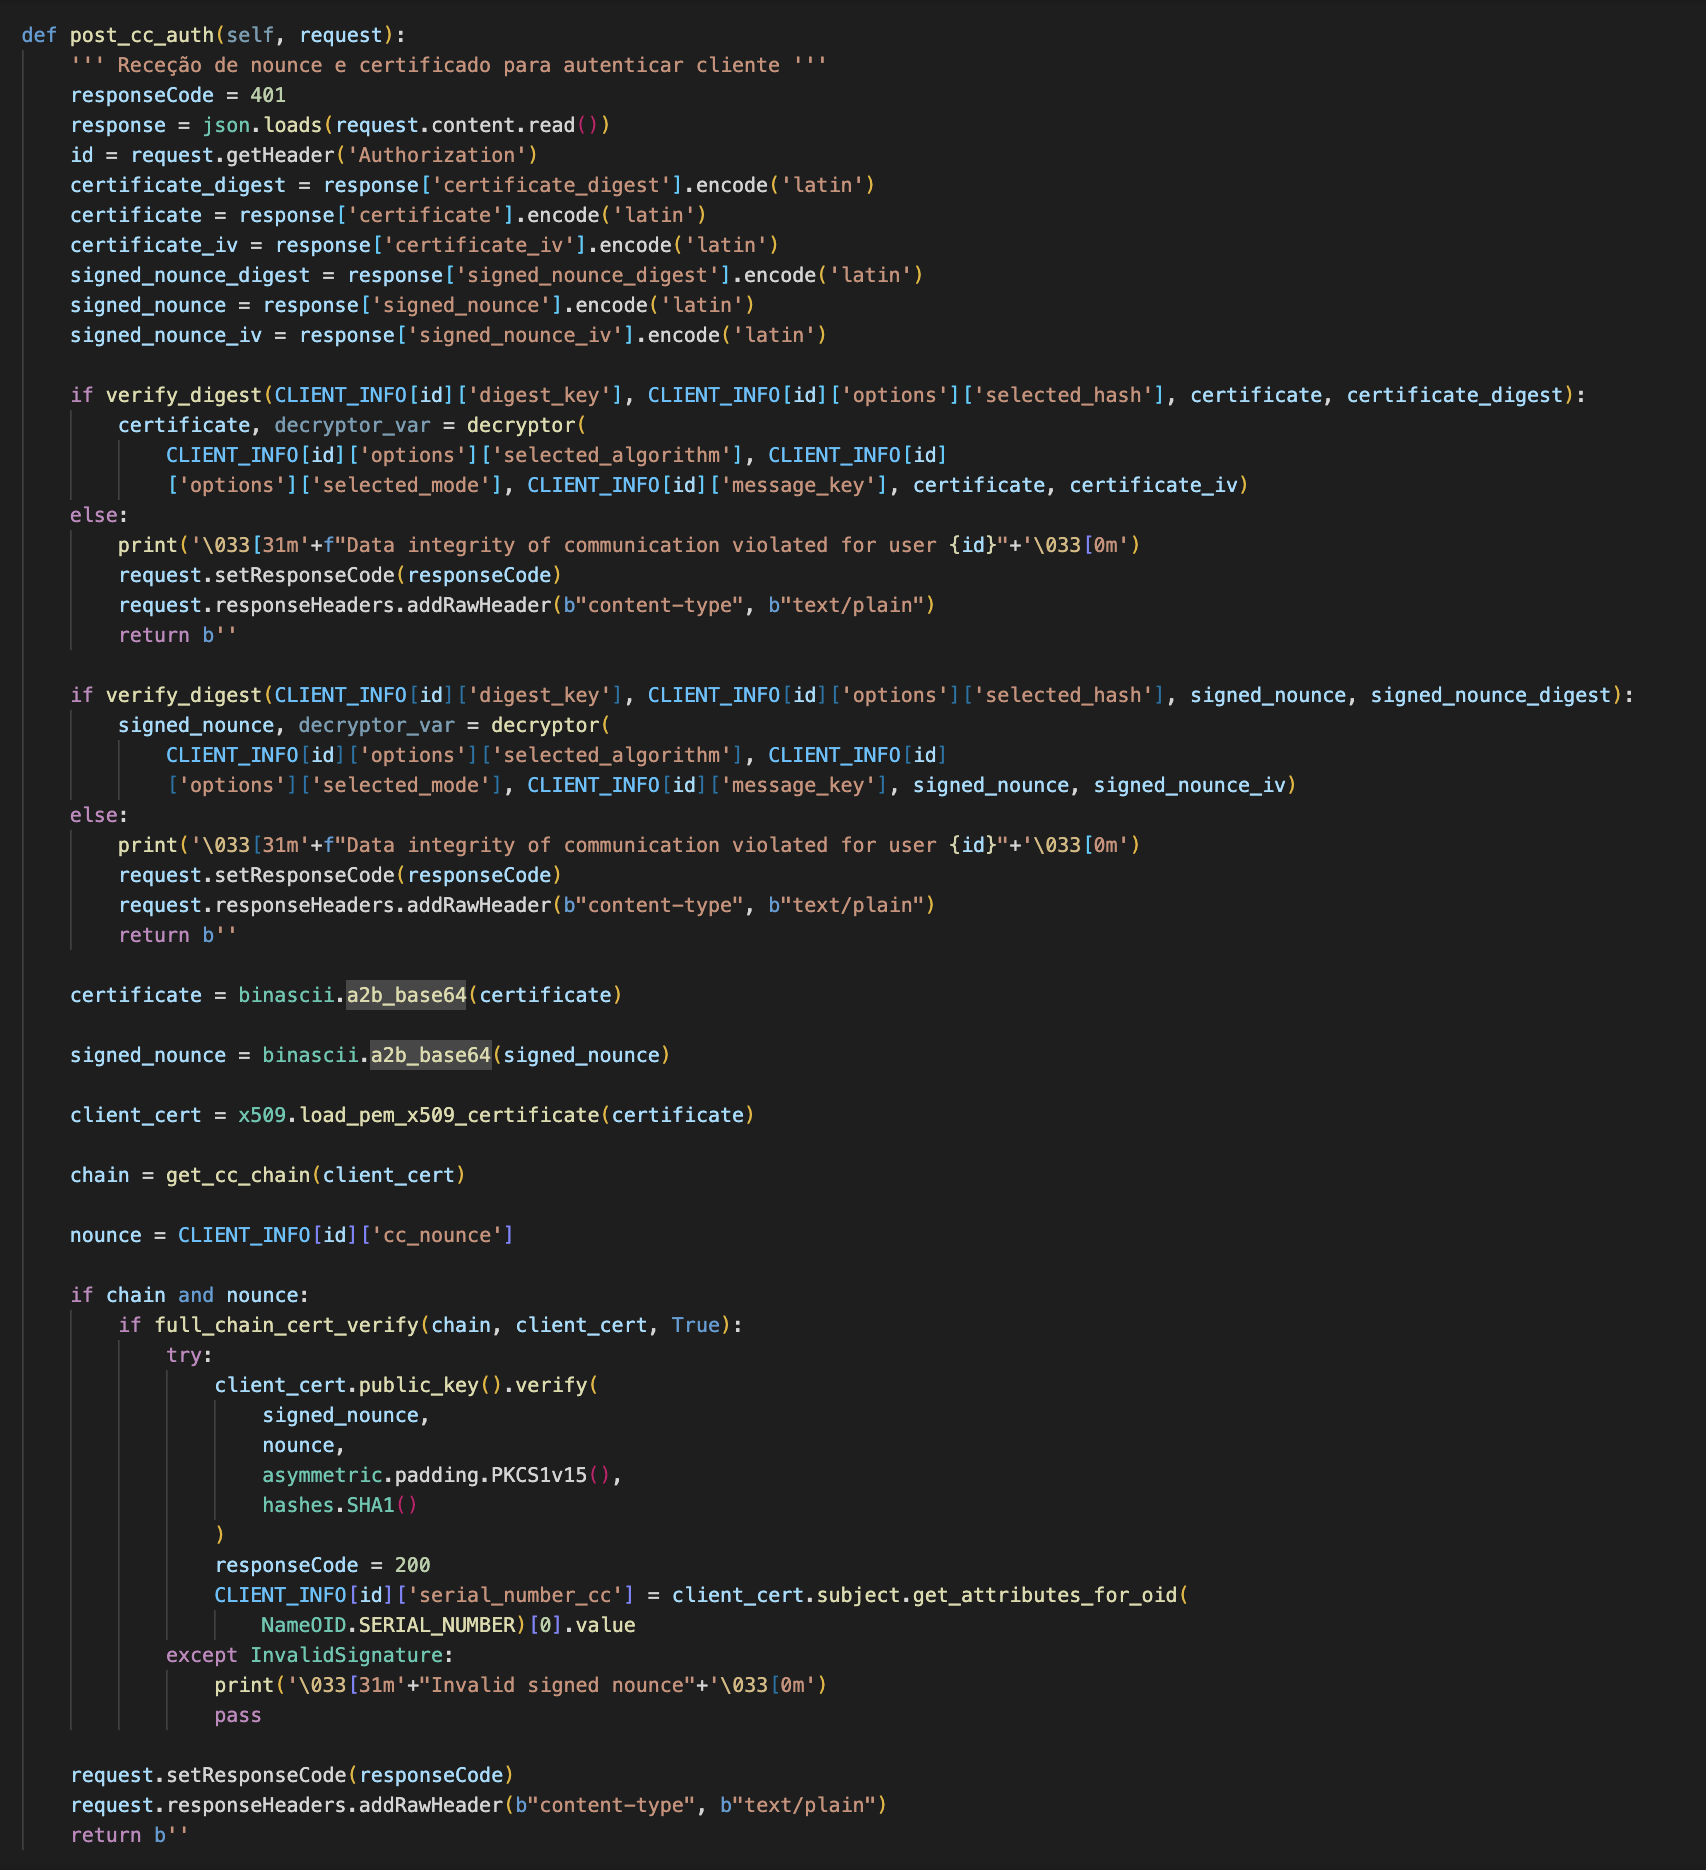
\includegraphics[width=\textwidth]{images/post_cc_auth_server.png}
        \caption{Processo de autenticação do cliente, no servidor}
\end{figure}

\par Ao validar a cadeia de certificação, o servidor cria a própria cadeia de certificação do certificado do cartão de cidadão, recorrendo à função \textit{get\_cc\_chain}, que percorre todos os certificados, verificando se algum deles é a entidade emissora do certificado passado e terminando quando encontra um certificado raiz, criando assim a cadeia.

\begin{figure}[!h]
        \centering
        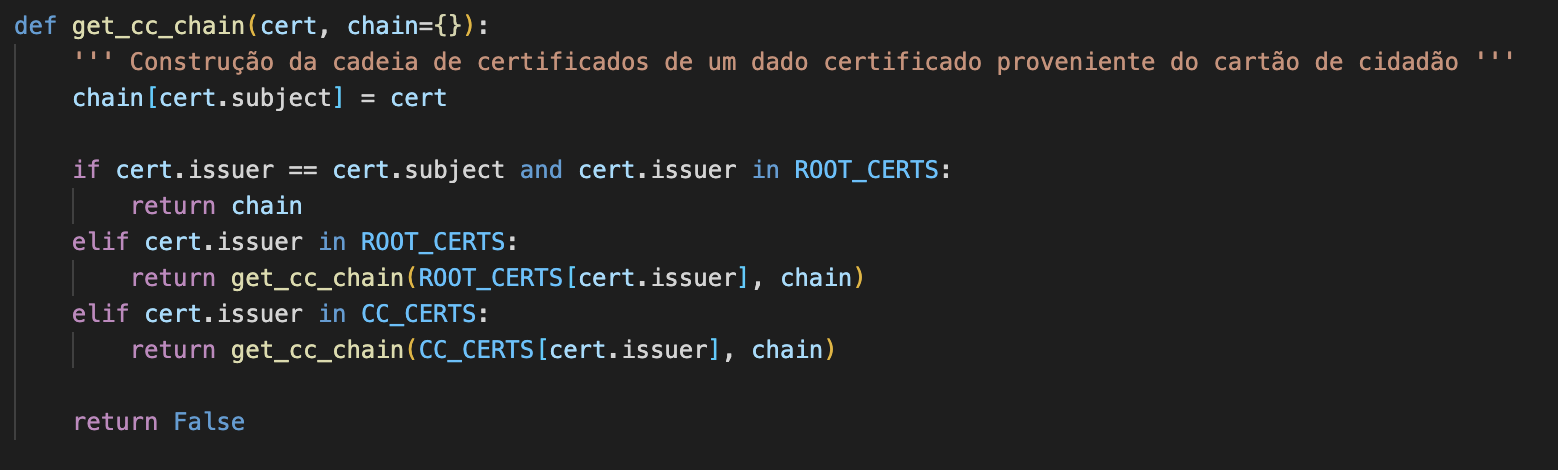
\includegraphics[width=300]{images/get_cc_chain.png}
        \caption{Criação da cadeia de certificação do certificado do cartão de cidadão}
\end{figure}

\par Existindo esta cadeia de certificação, o servidor verifica que todos os certificados estão válidos, de forma semelhante à feita pelo cliente mas, desta vez, verificando também com as listas de revogação carregadas. Neste caso, o objetivo dos certificados terá de ser do tipo \textit{digital\_signature} no certificado do cartão de cidadão, visto que é utilizado para verificar assinaturas sem ser de certificado e, do tipo \textit{key\_cert\_sign} nos restantes, visto que são utilizados para verificar assinaturas de outros certificados:

\begin{figure}[!h]
        \centering
        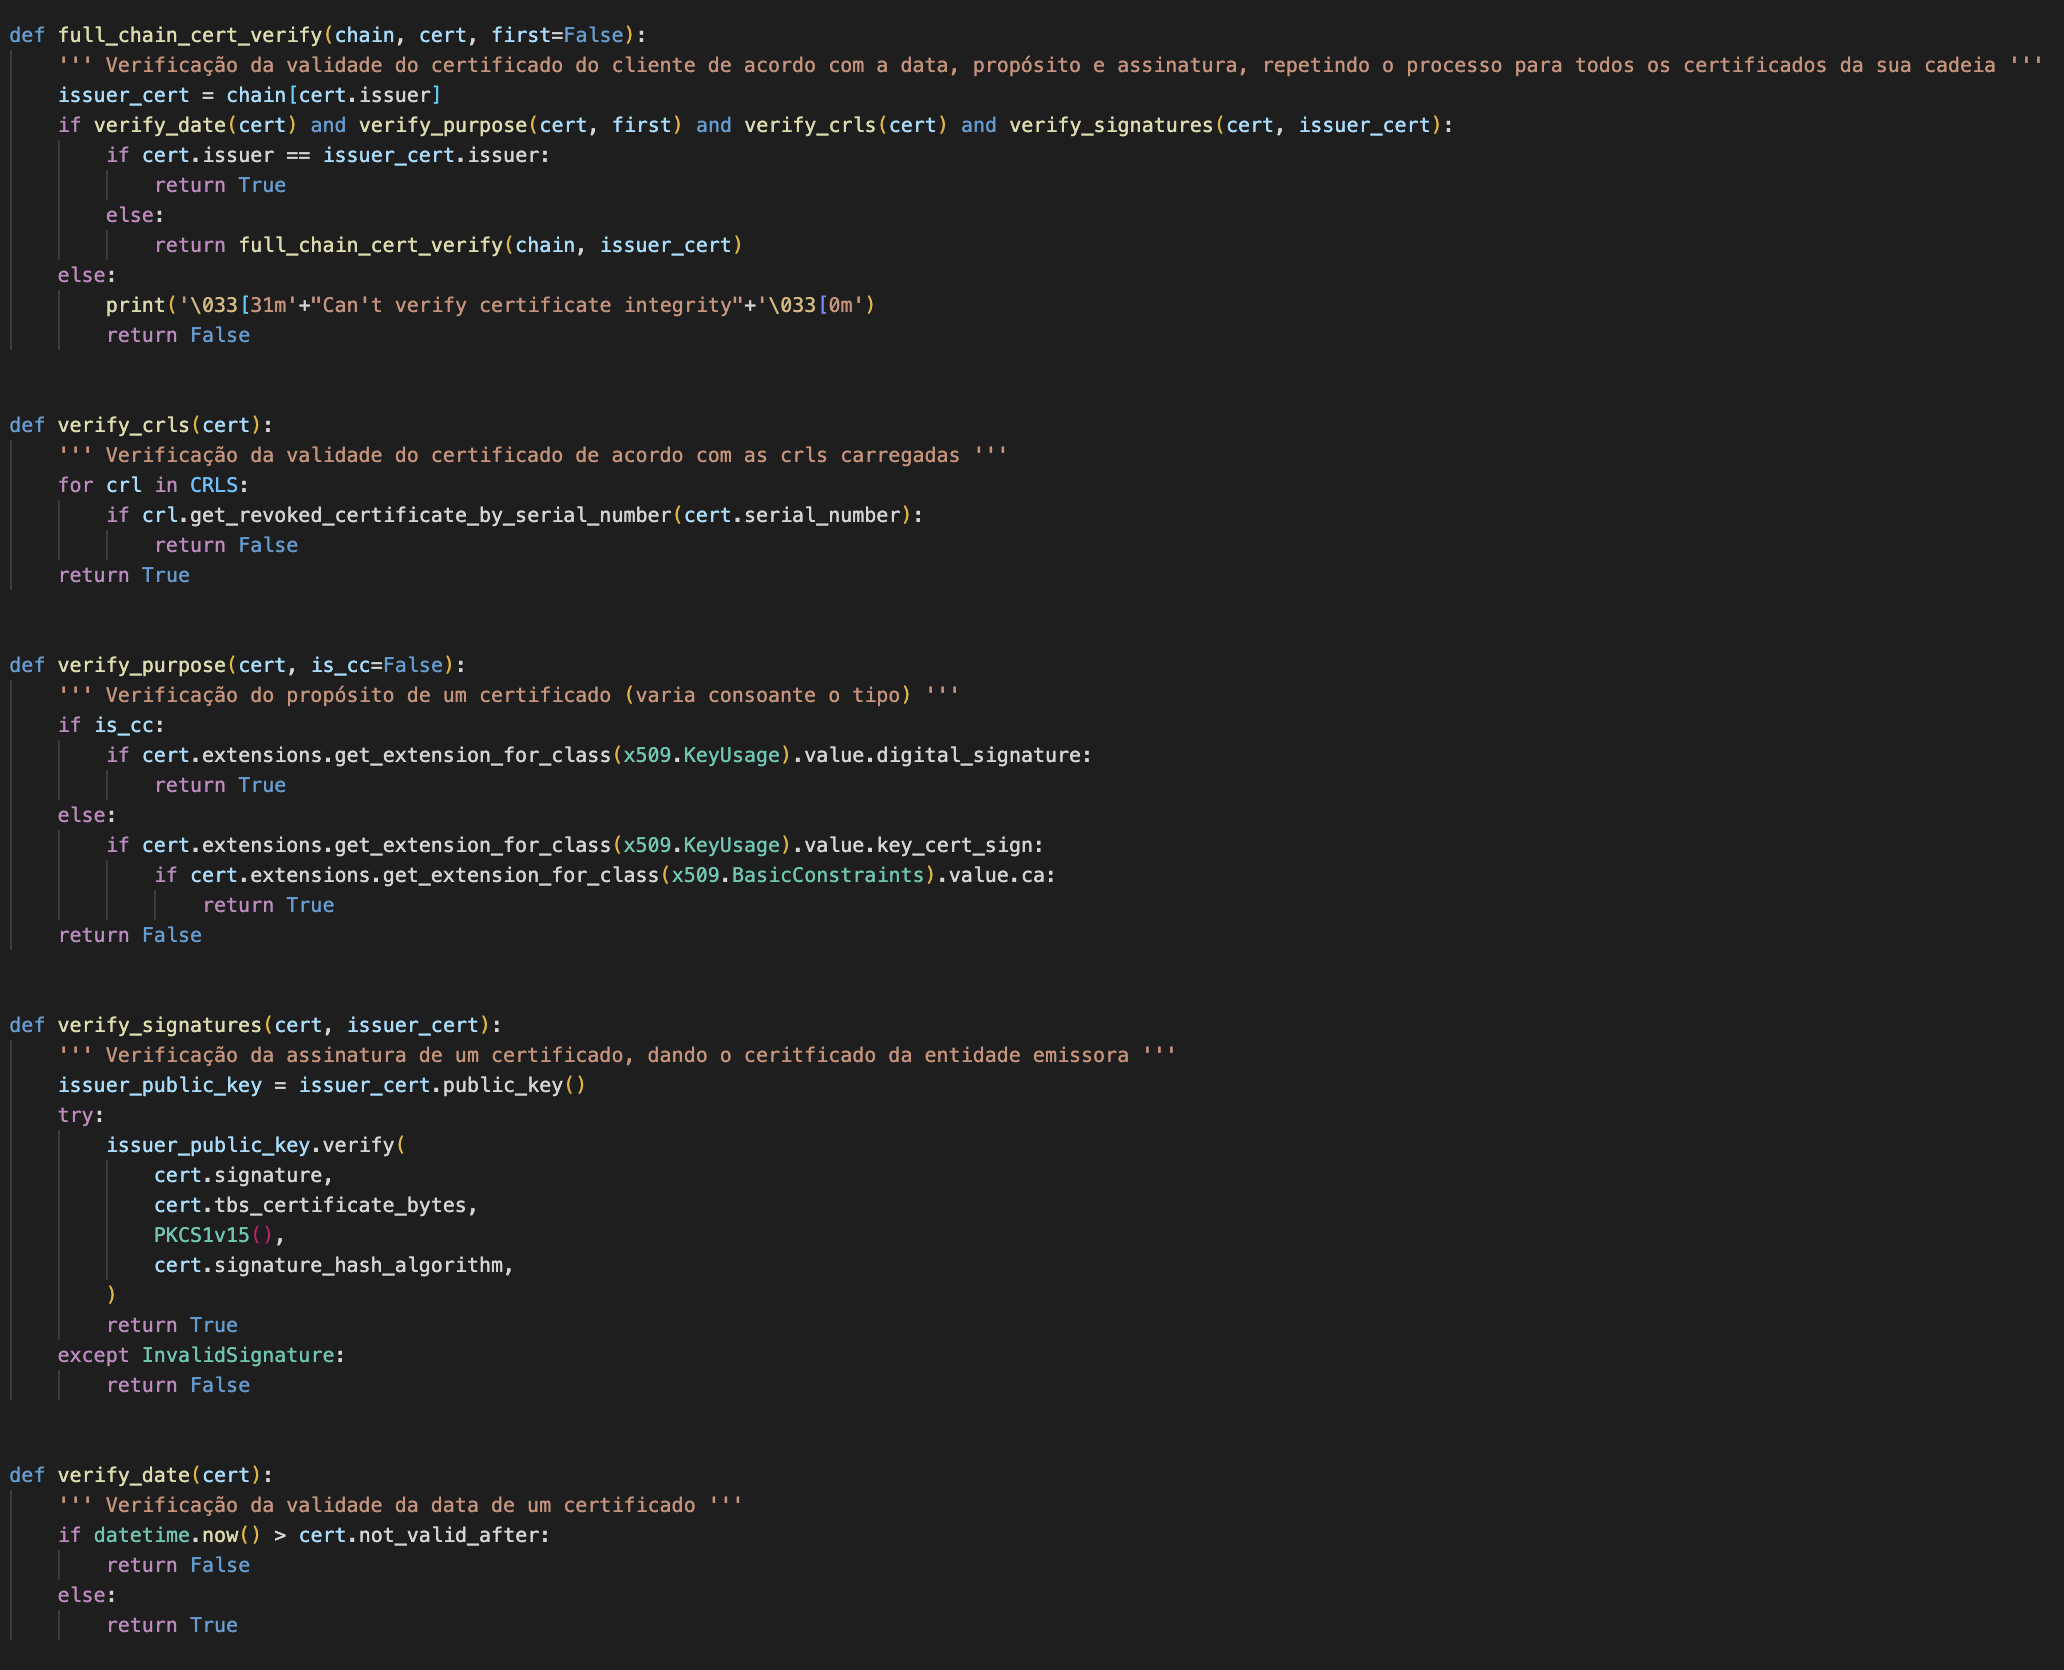
\includegraphics[width=400]{images/chain_verify_server.png}
        \caption{Validação da cadeia de certificação}
\end{figure}

\par Estando este processo concluído em conformidade, o cliente passa a estar autenticado para com o servidor.

\clearpage

\subsection{Licenças e Autenticação das mesmas}

\par Ultrapassadas todas as medidas de seguranças mencionadas anteriormente, o programa pode finalmente mostrar ao cliente as músicas disponíveis e, caso não tenha acesso, permitir a compra de músicas através da geração de uma licença com tempo limitado.

\par Para isso, é feito um pedido ao servidor de modo a listar as músicas disponíveis. Nesta listagem é também apresentado se o cliente possui acesso à música ou não, de acordo com as licenças geradas anteriormente e com as informações provenientes da autenticação do cliente:

\begin{figure}[!h]
        \centering
        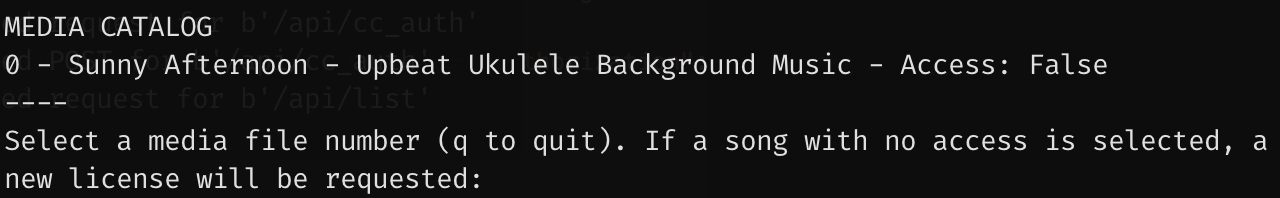
\includegraphics[width=250]{images/catalog_running.png}
        \caption{Exemplo de listagem de músicas ao executar o programa do cliente}
\end{figure}

\par Toda esta informação é apresentada com a seguinte implementação:

\begin{figure}[!h]
        \centering
        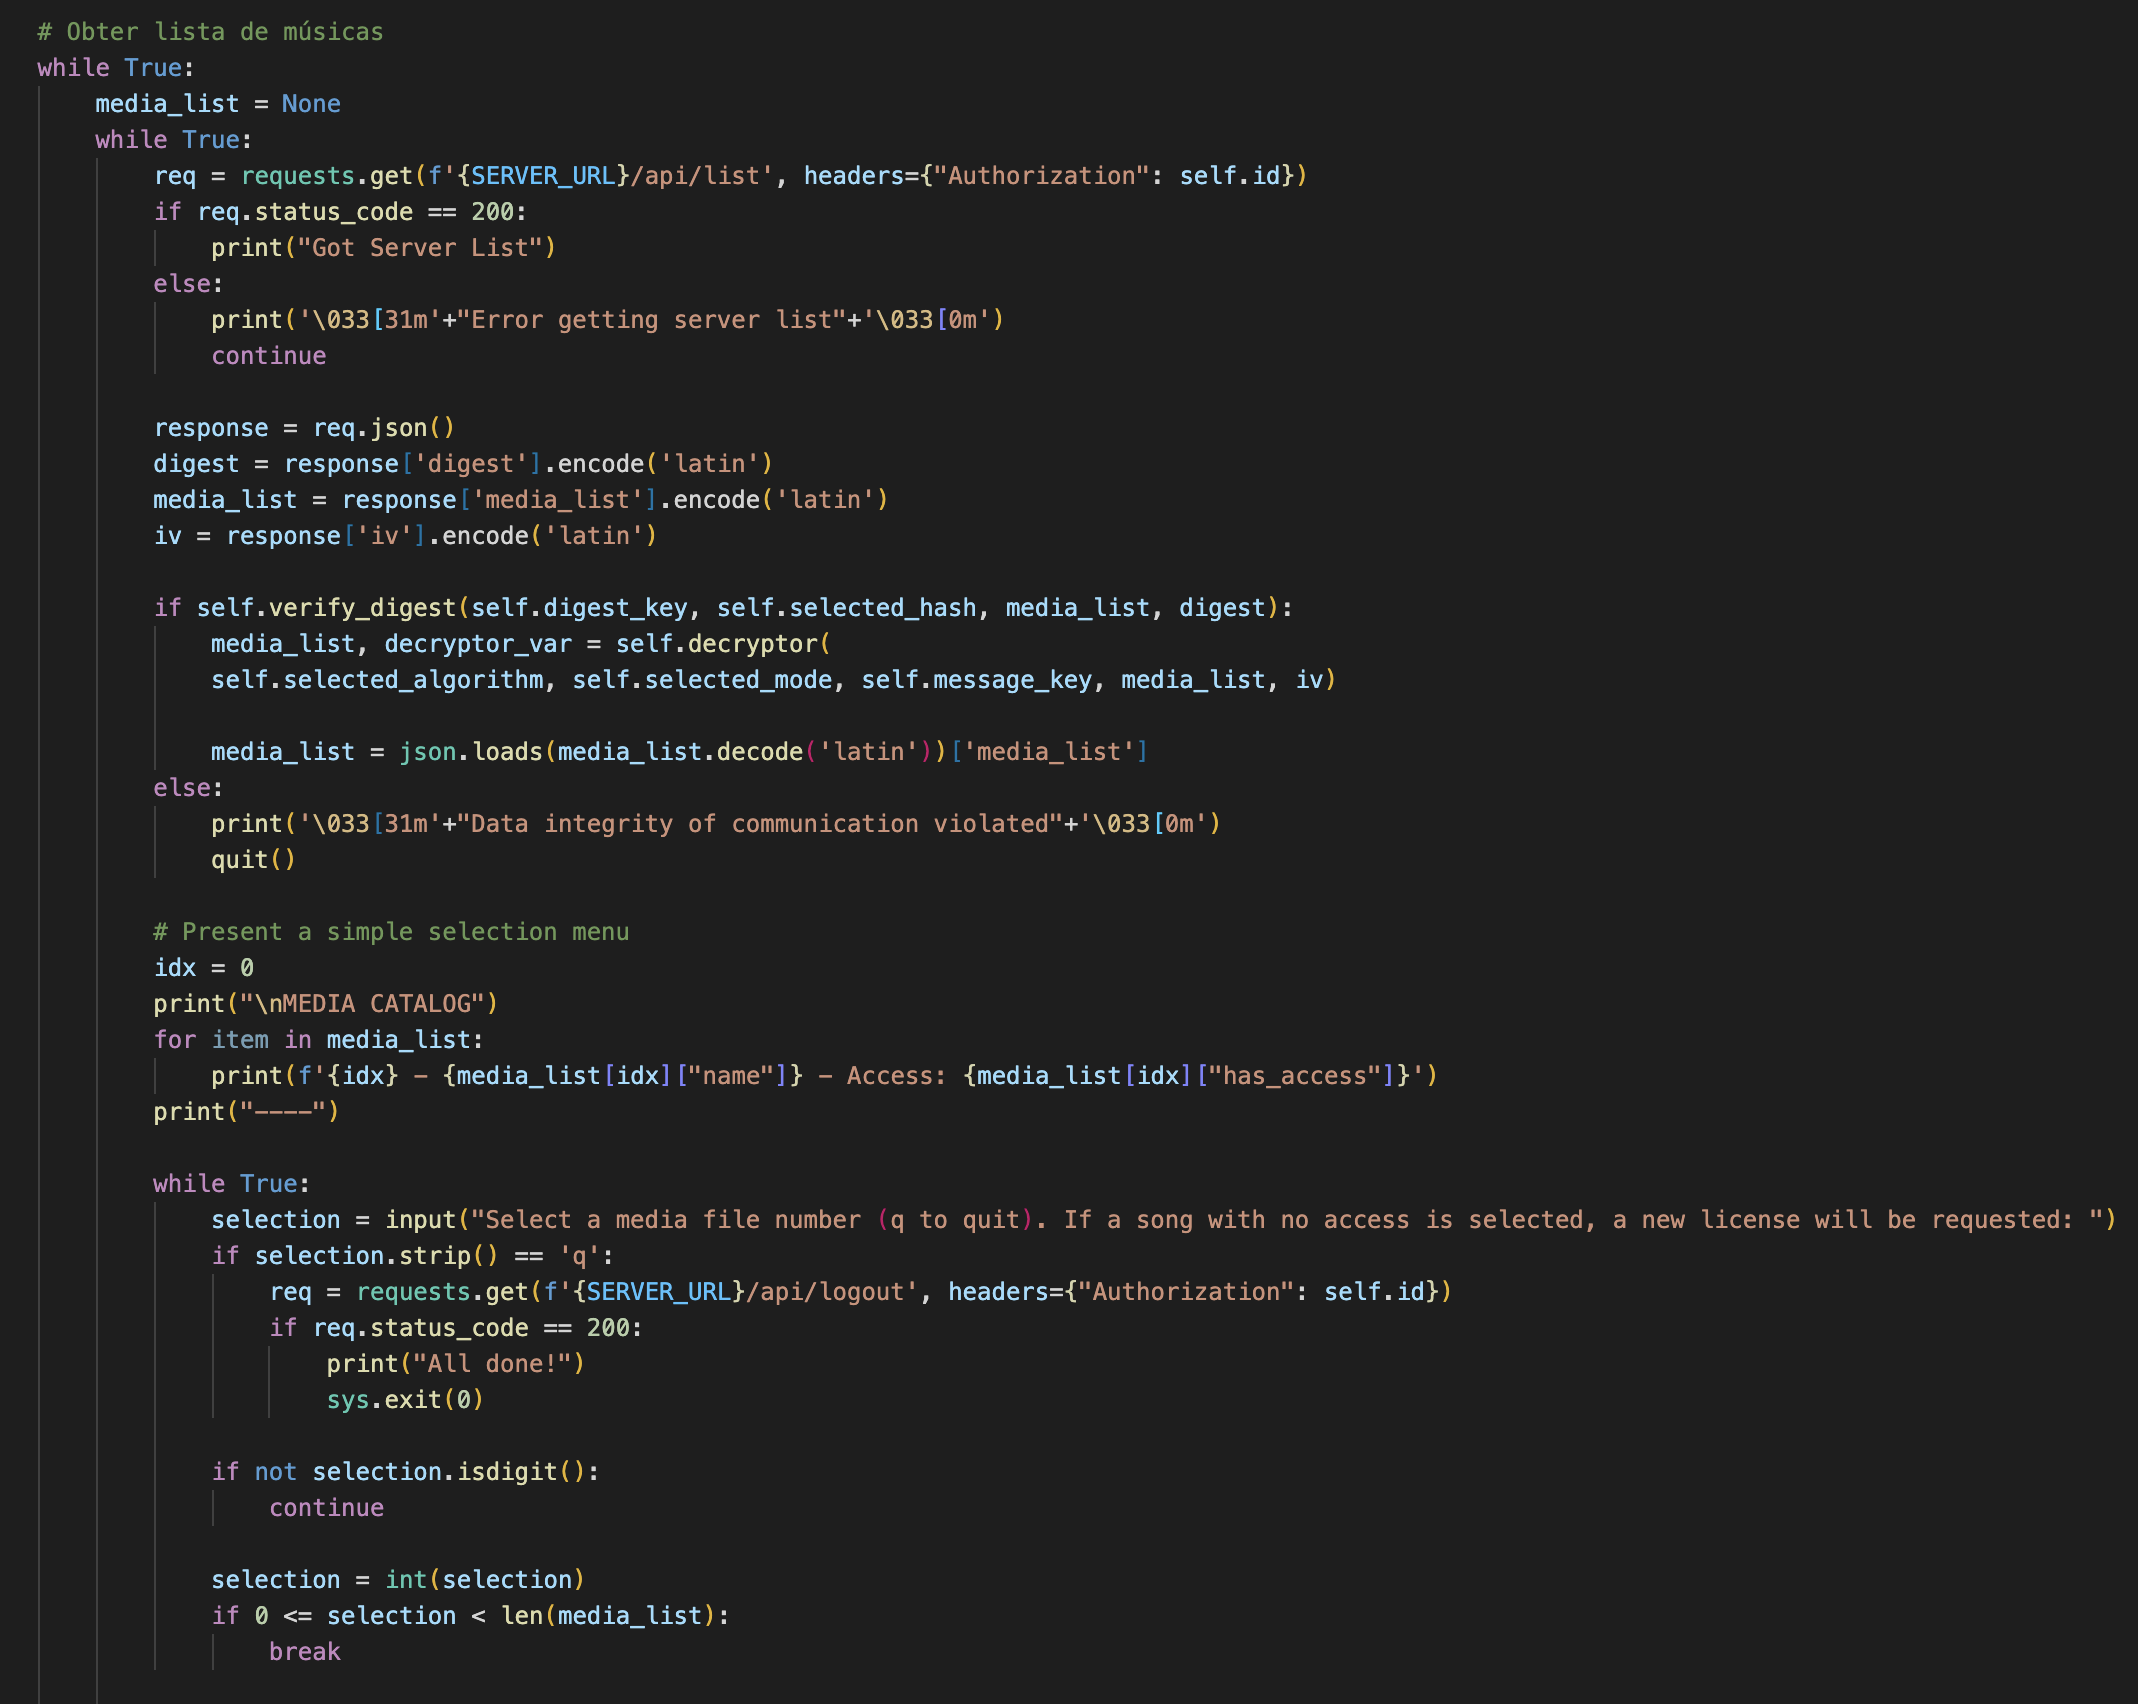
\includegraphics[width=450]{images/get_list_client.png}
        \caption{Obter lista de músicas no cliente}
\end{figure}

\par Caso o cliente não tenha permissão para ouvir uma certa música, ao seleccionar essa música, irá fazer um pedido ao servidor para gerar uma nova licença, sendo que o servidor gerará uma licença com validade de 1 hora, permitindo ao utilizador ouvir a música na próxima hora, como será explicado posteriormente. Esta licença contém, também, no final, separado por \textit{b"-"}, a assinatura da mesma feita pelo servidor. A validade da licença depende da assinatura, sendo que ao receber a licença, o cliente confirma se a assinatura é válida antes de a guardar em \textit{client/licenses}. Apesar da licença guardada pelo utilizador não ser utilizada, permite que o servidor não consiga refutar a mesma em casos extremos:

\begin{figure}[!h]
        \centering
        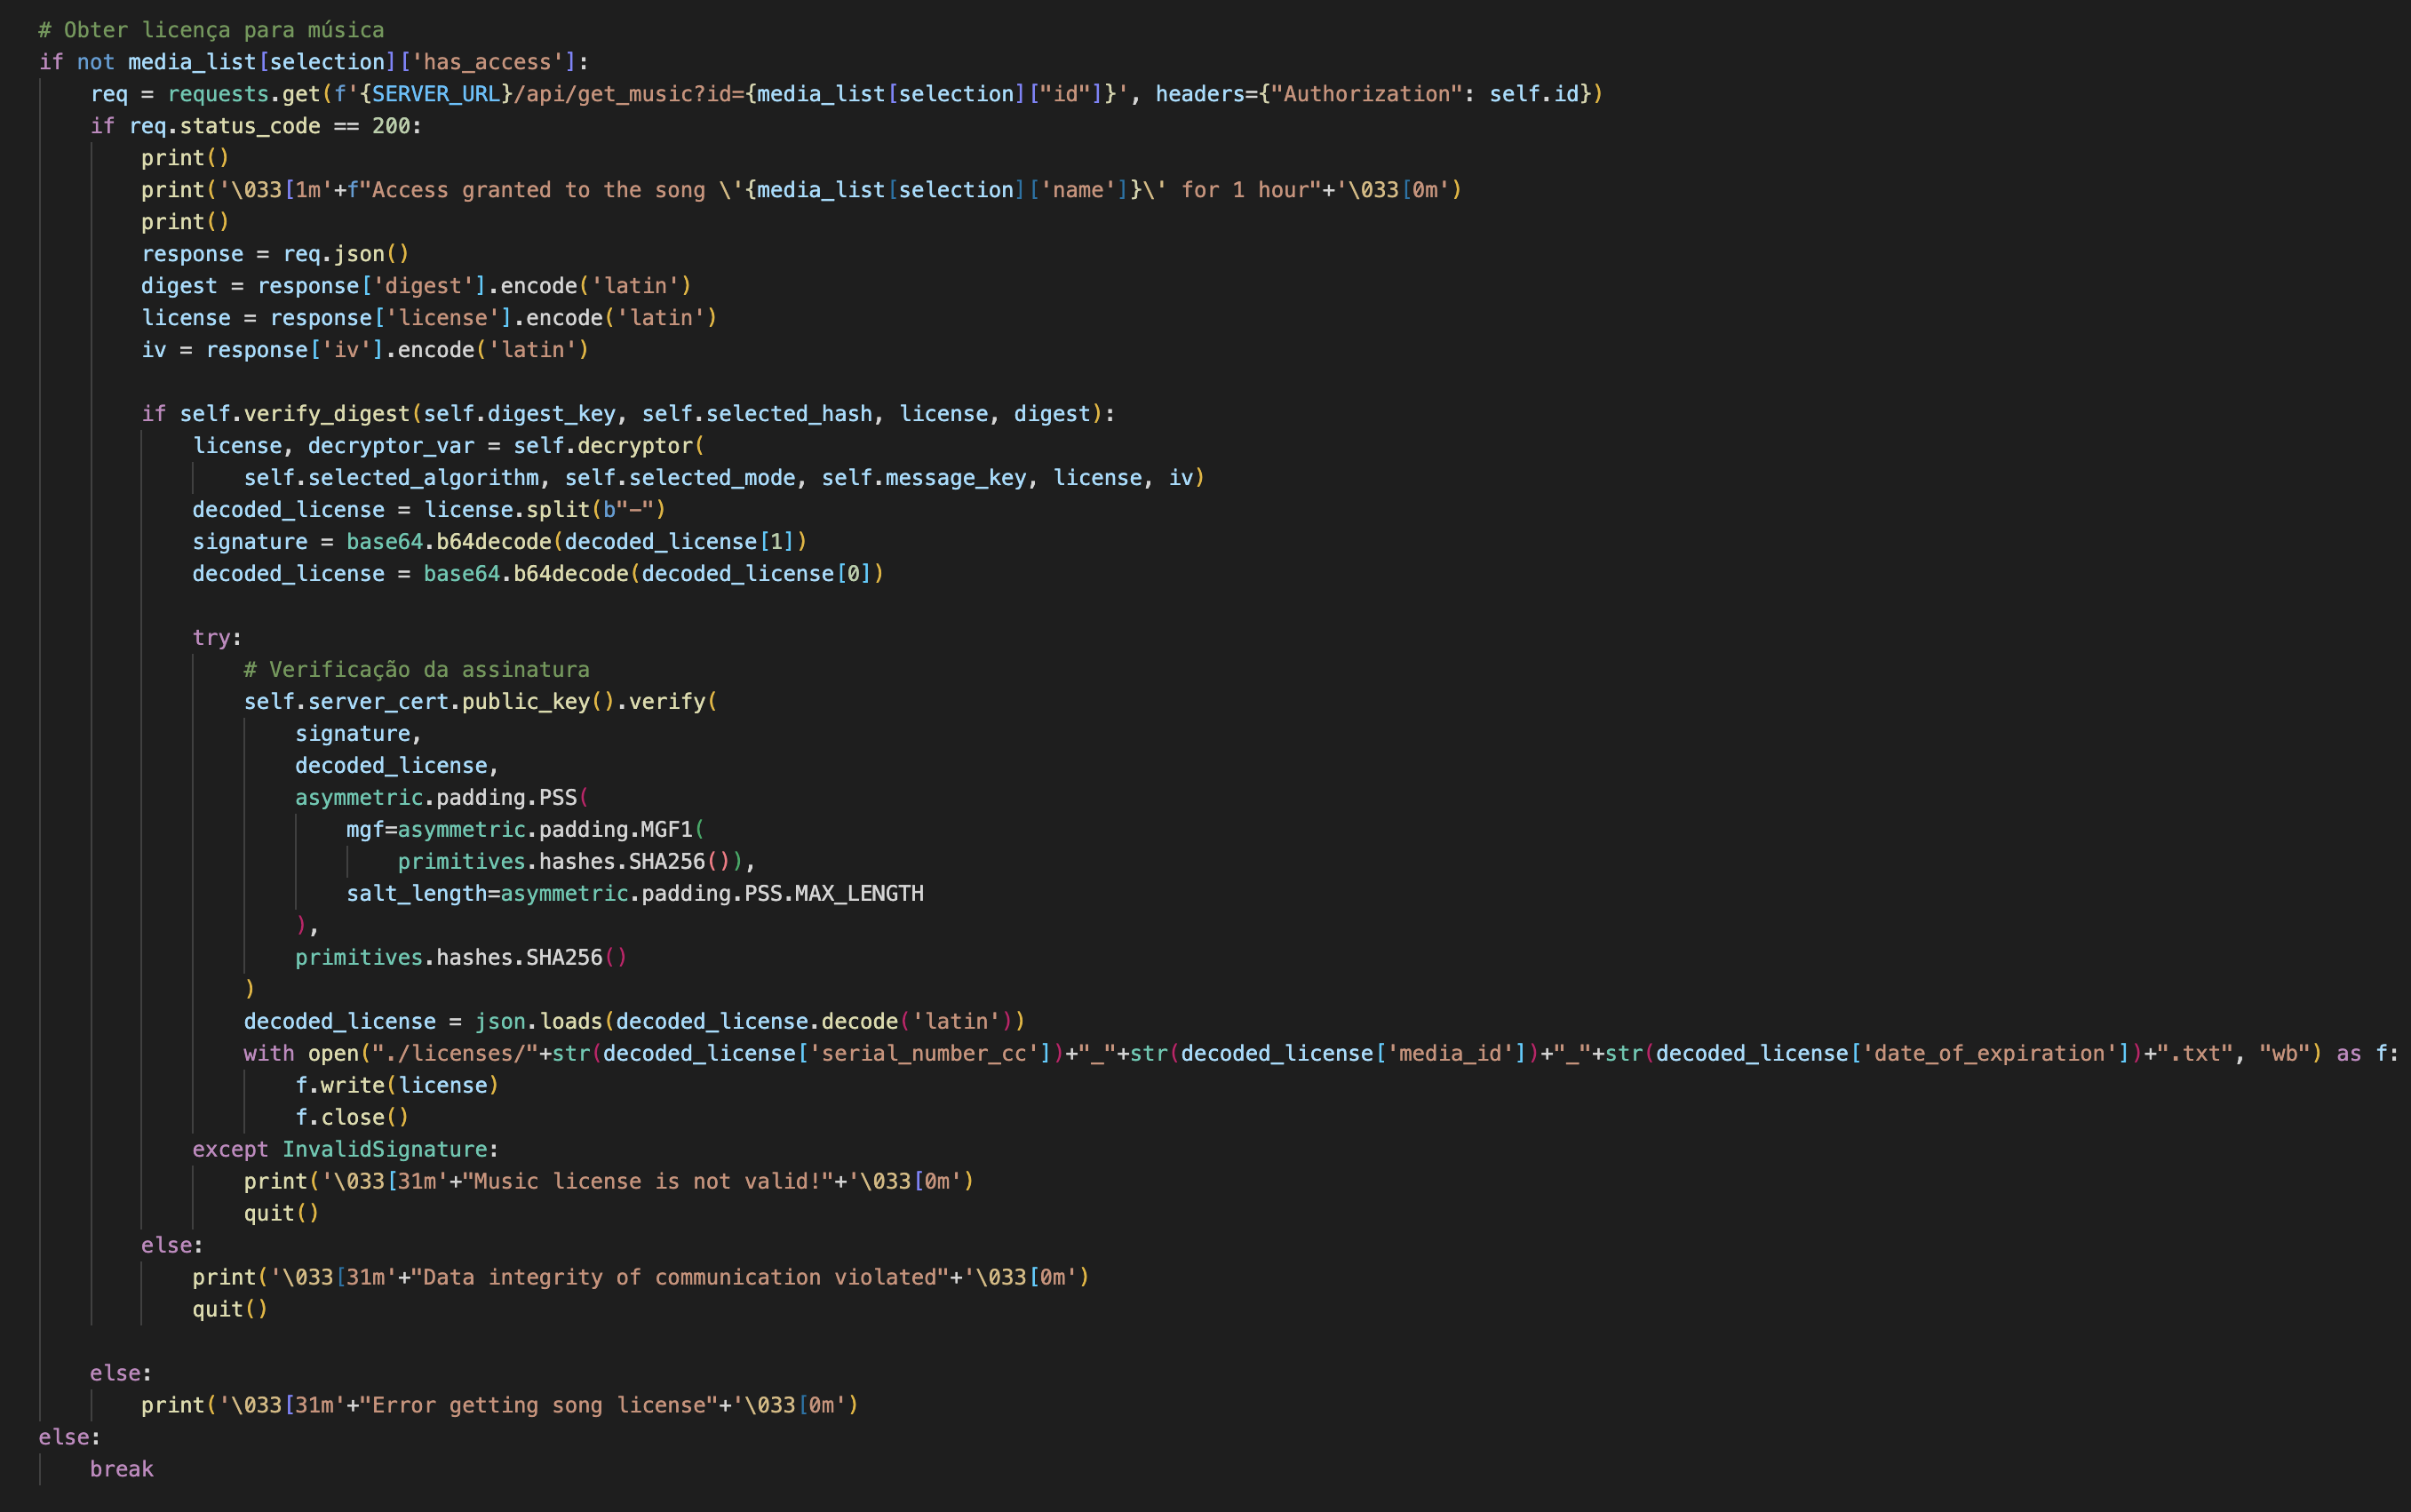
\includegraphics[width=\textwidth]{images/get_license_client.png}
        \caption{Obter licença de músicas no cliente}
\end{figure}

\par No servidor, é gerada essa licença e guardada em \textit{server/licenses}, sendo que o nome do ficheiro é constituído pelo \textit{serial\_number\_cc}, \textit{media\_id} e \textit{date\_of\_expiration} para permitir uma verificação prévia à abertura do ficheiro e verificação da assinatura.

\par A licença é um objeto \textit{JSON} com as seguintes propriedades:

\begin{itemize}
    \item \textbf{serial\_number\_cc} - O número do cartão de cidadão, que é guardado no servidor durante a autenticação do utilizador em comunicação cifrada
    \item \textbf{media\_id} - O identificador da música em questão
    \item \textbf{date\_of\_expiration} - Data até quando a licença é válida
\end{itemize}

\clearpage

\begin{figure}[!h]
        \centering
        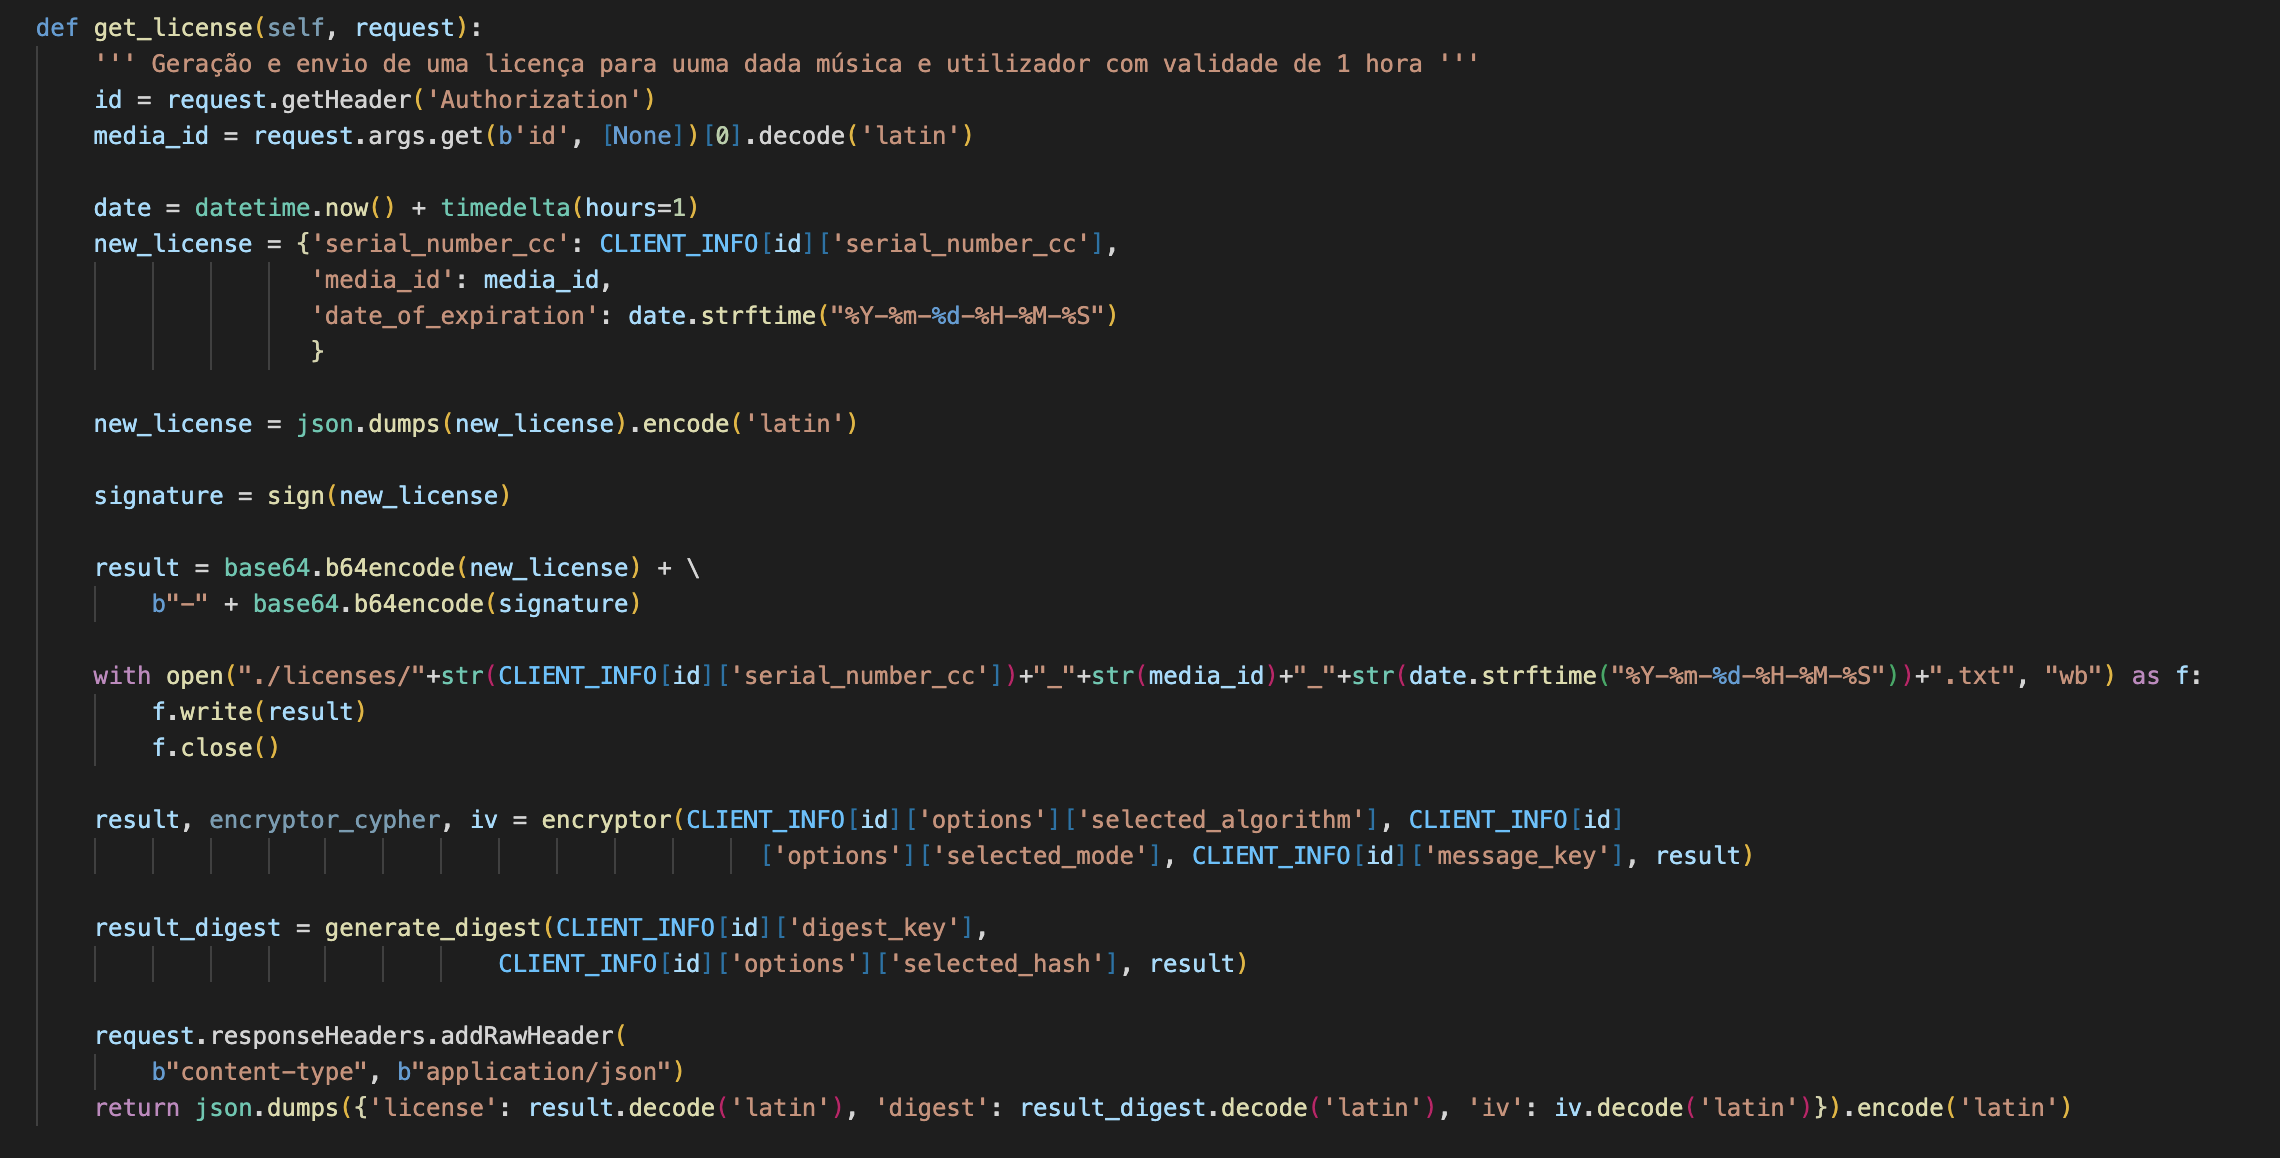
\includegraphics[width=\textwidth]{images/get_license_server.png}
        \caption{Geração licença de músicas no servidor}
\end{figure}

\par Com a licença gerada, quando o cliente ouvir uma música, o servidor verifica em todos os pedidos de cada \textit{bloco} da música se o cliente continua a ter uma licença válida:

\begin{figure}[!h]
        \centering
        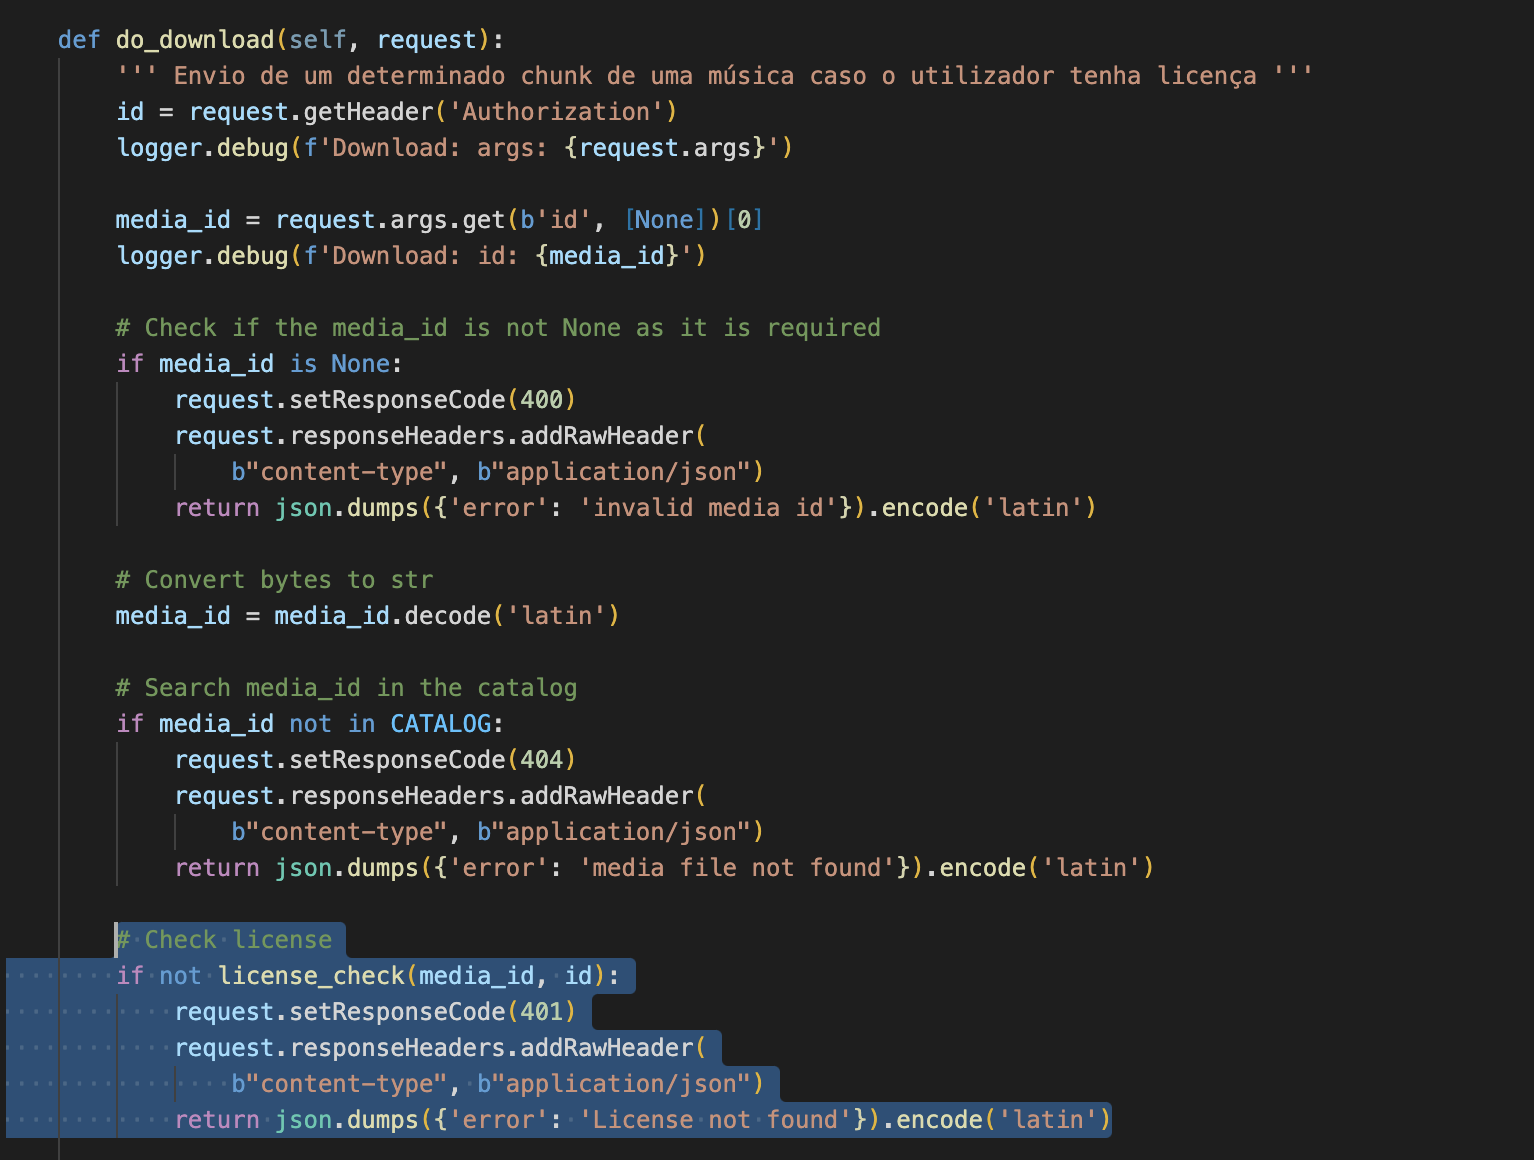
\includegraphics[width=325]{images/do_download_license.png}
        \caption{Verificação (parte assinalada) da licença ao enviar \textit{blocos} de músicas, no servidor}
\end{figure}

\clearpage

\par A verificação das licenças do lado do servidor percorre todas as licenças guardadas, faz uma verificação inicial segundo o nome do ficheiro e, em caso positivo, abre o ficheiro e verifica as informações no objeto \textit{JSON} e a validade da assinatura:

\begin{figure}[!h]
        \centering
        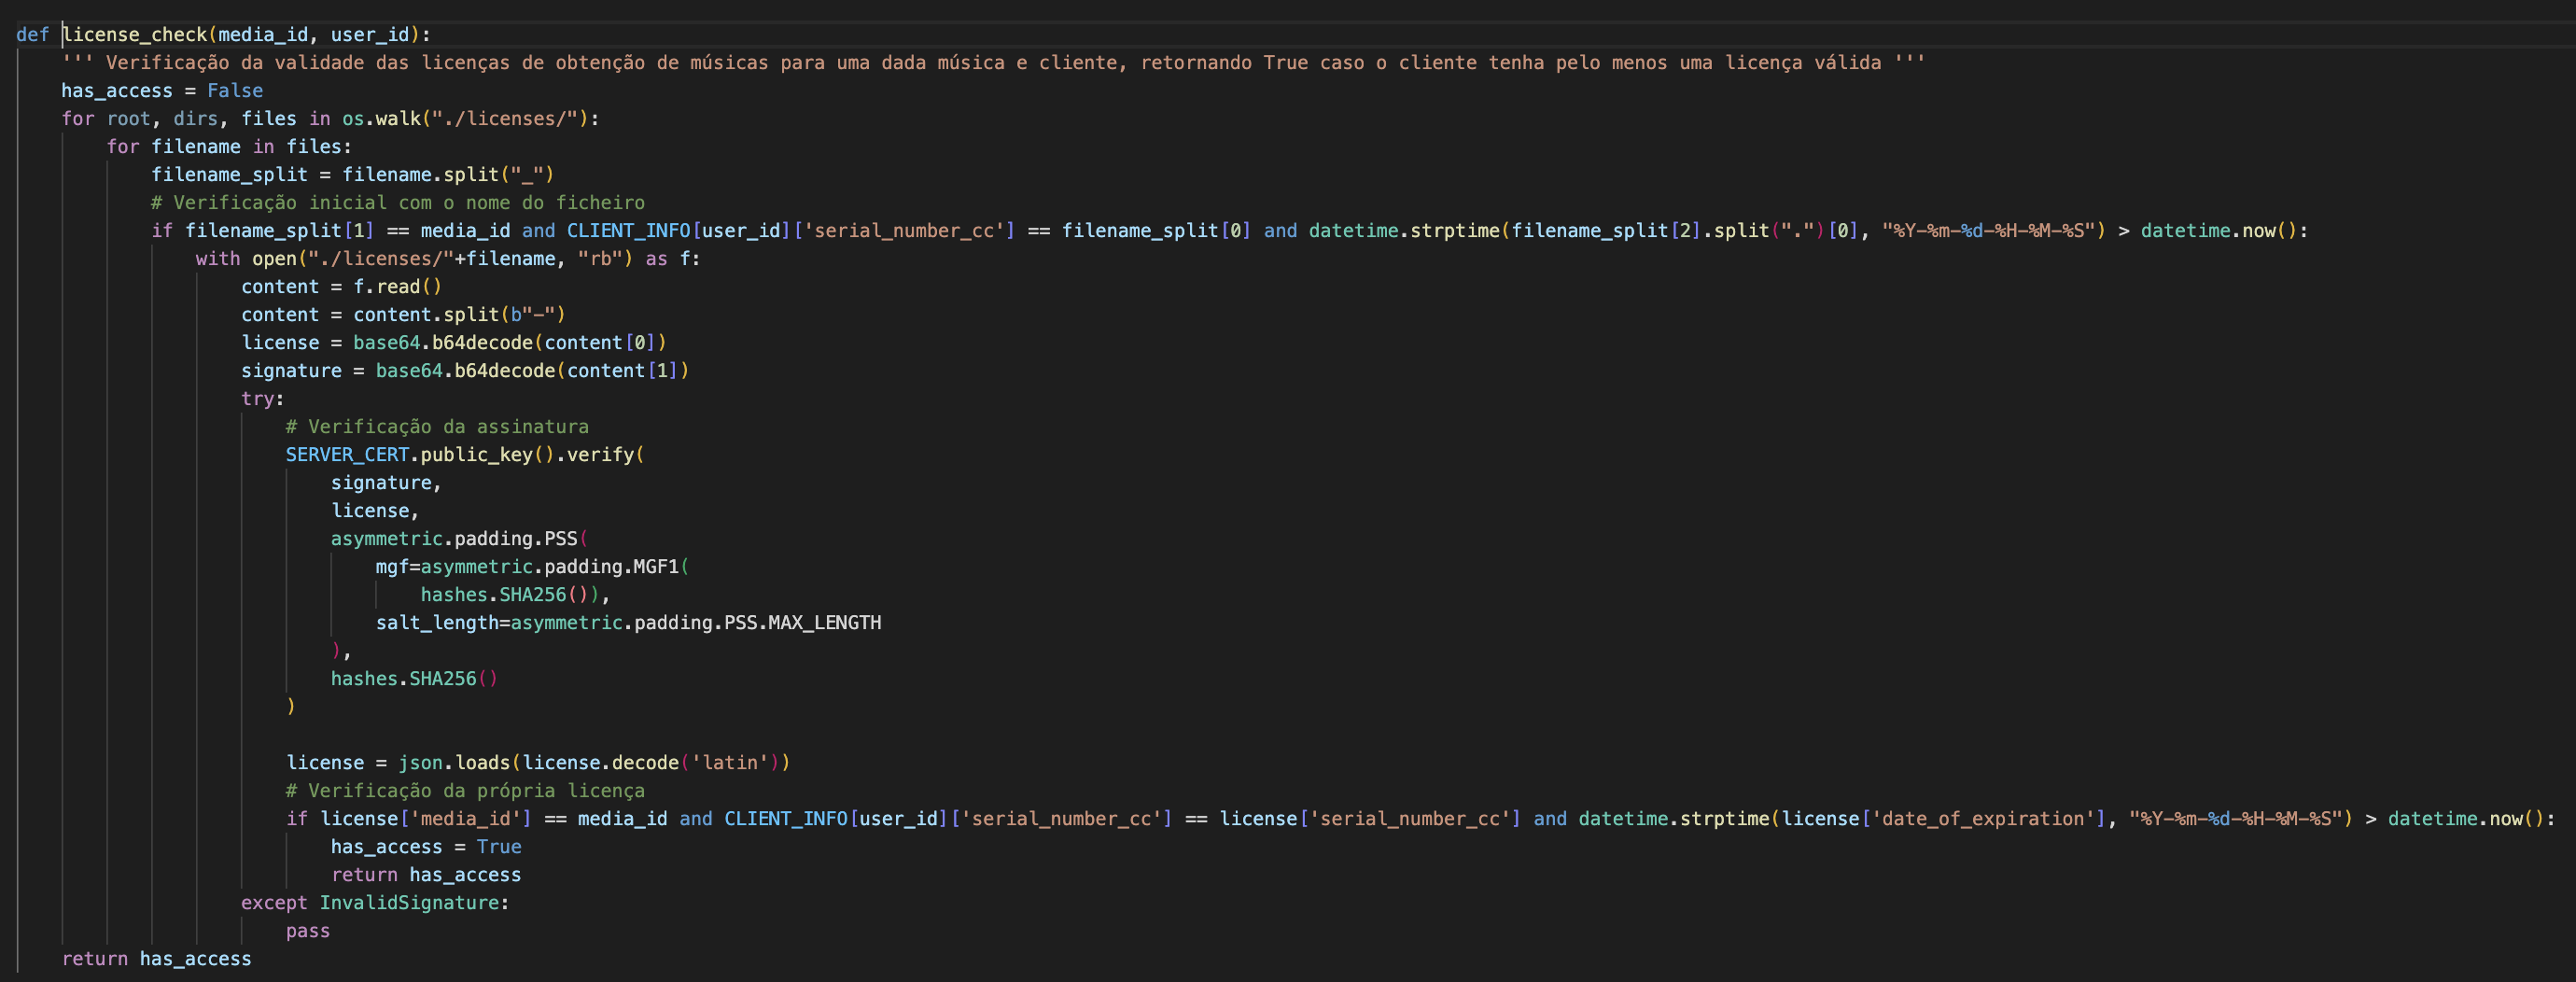
\includegraphics[width=\textwidth]{images/check_license_server.png}
        \caption{Função de verificação da validade de licenças dada uma música e um utilizador, no servidor}
\end{figure}


\clearpage

\subsection{Proteção do conteúdo guardado no servidor}
\subsubsection{Encriptação}
\par No âmbito da proteção dos ficheiros a nível do servidor foi desenvolvido um \textit{script} independente, \textit{file\_encrypt.py} em \textit{/server}, o qual tem que ser executado antes de iniciar o servidor caso as músicas ainda não estejam cifradas.

\par Através deste \textit{script}, é efetuada a encriptação dos ficheiros segundo uma cifra híbrida e são guardadas as versões protegidas no diretório \textit{/server/encrypted\_catalog}, sendo ainda realizada a geração de um documento de texto com a informação que o servidor necessita para proceder à desencriptação, nomeadamente, nome do ficheiro, chave simétrica utilizada para encriptação das músicas e \textit{iv} utilizado.

\par Primeiramente é percorrido o diretório \textit{/server/catalog} e para cada música é efetuada uma encriptação com chave simétrica, segundo o algoritmo \textit{AES} e modo de cifra \textit{OFB}, utilizando uma chave e \textit{iv} aleatórios. Após a cifra os novos documentos são guardados em \textit{/server/encrypted\_catalog}.

\begin{figure}[!h]
        \centering
        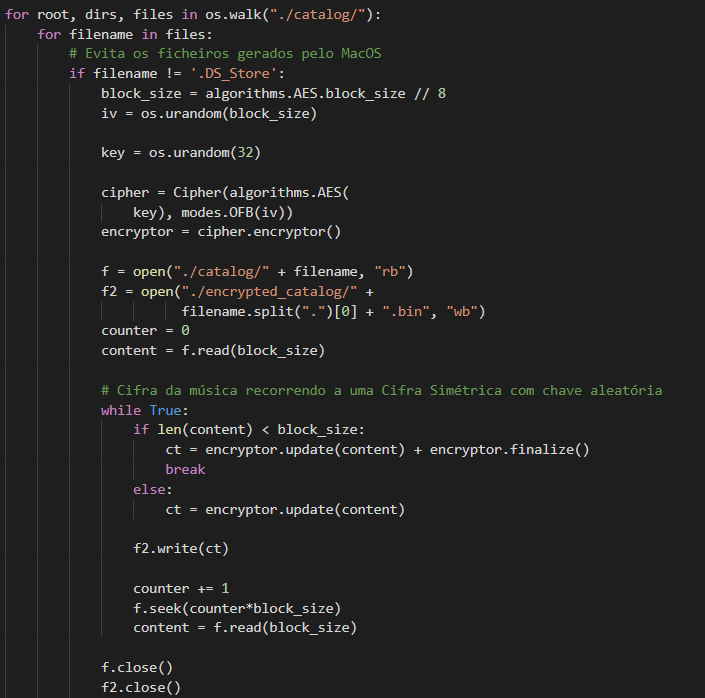
\includegraphics[width=400]{images/Encriptação das músicas.png}
        \caption{Processo de encriptação das músicas.}
\end{figure}

\par Posteriormente é gerado um documento de texto, \textit{file\_info.txt} no diretório \textit{/server}, que para cada música contém o nome do ficheiro, a chave de encriptação cifrada através da chave pública do servidor e o \textit{iv} utilizados na cifra simétrica dessa música. Desta forma foi utilizada cifra simétrica para cifrar os ficheiros e cifra assimétrica para cifra a chave simétrica, juntando o melhor dos dois mundos.

\begin{figure}[!h]
        \centering
        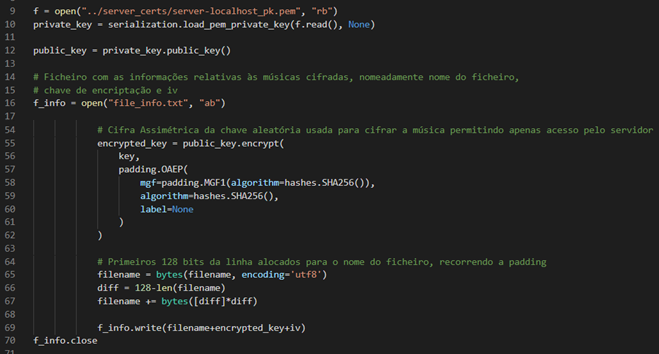
\includegraphics[width=500]{images/Geração de file info.png}
        \caption{Geração do documento file\_info.txt }
\end{figure}

\subsubsection{Desencriptação}
\par Ao iniciar o servidor é chamada a função \textit{decrypt\_catalog()}, que irá por sua vez proceder à leitura da informação contida em \textit{file\_info.txt}, desencriptará as chaves simétricas utilizadas através da chave privada do servidor e poderá de seguida desencriptar os ficheiros das músicas e guardá-los em memória \textit{RAM} onde estarão seguros, mais exatamente no dicionário SONGS.
\par Esta solução simplificada foi adotada no âmbito do projeto uma vez que não compromete a segurança visto que a memória \textit{RAM} é volátil, no entanto reconhecemos que numa situação real representaria um problema a nível de escalabilidade do serviço, podendo ser interessante aplicar outro modo de cifra, como o \textit{CBC}, apenas necessitando do bloco anterior ao que se pretende para ser possível desencriptar.

\begin{figure}[!h]
        \centering
        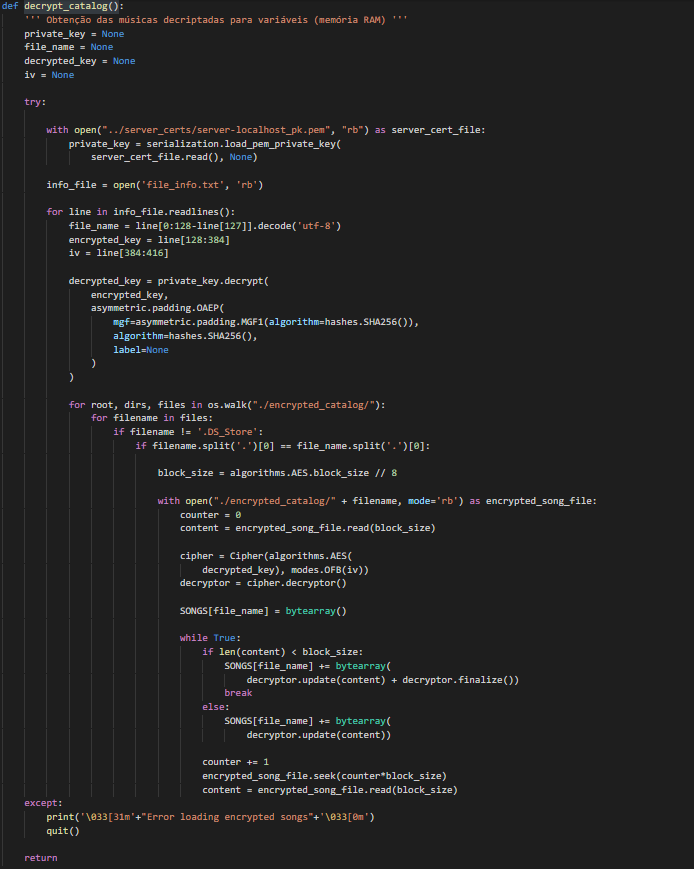
\includegraphics[width=500]{images/Decrypt catalog.png}
        \caption{Função decrypt\_catalog()}
\end{figure}


\clearpage


\section{Conclusão}

\par Bla bla

\clearpage

\section{Bibliografia}

\bibliographystyle{plain}

\bibliography{biblist}

\vspace{5mm} %5mm vertical space

[1] \url{http://cryptowiki.net/index.php?title=The_Double_Ratchet_Algorithm}

[2] \url{https://www.youtube.com/watch?v=9sO2qdTci-s}

[3] \url{https://www.ecce.gov.pt/certificados/}

[4] \url{https://pki.cartaodecidadao.pt}

[5] \url{https://cryptography.io/en/latest/index.html}

\par Para além destes \textit{websites}, foi utilizada muita informação proveniente dos slides e guiões das aulas teóricas e práticas.


\end{document}

